\documentclass[11pt]{article}
% Shared packages, macros, and page setup for the project log.
\usepackage[a4paper,margin=2.5cm]{geometry}
\usepackage[utf8]{inputenc}
\usepackage[T1]{fontenc}
\usepackage{graphicx}
\usepackage{booktabs}
\usepackage{amsmath}
\usepackage{xcolor}
\usepackage{caption}
\usepackage{subcaption}
\usepackage[colorlinks=true,linkcolor=blue!50!black,citecolor=blue!50!black,urlcolor=blue!50!black]{hyperref}
\usepackage{parskip}

% \finding{text} -- a highlighted callout for a discovery worth remembering at a glance.
\newcommand{\finding}[1]{%
  \par\medskip\noindent
  \fcolorbox{black!20}{black!4}{%
    \parbox{\dimexpr\linewidth-2\fboxsep-2\fboxrule}{\textbf{Finding.} #1}%
  }%
  \par\medskip
}

% \supersededby{label}{reason} -- a one-line forward pointer left on an old entry when a later
% entry revises or overturns it. The old entry's text is left otherwise unchanged; see
% "Revising earlier decisions and findings" in report_rules.md.
\newcommand{\supersededby}[2]{%
  \par\smallskip\noindent
  {\small\textcolor{black!55}{$\dagger$ \textbf{Superseded} --- see Section~\ref{#1}: #2}}%
  \par\smallskip
}

\usepackage{float}
\usepackage{tabularx}
\setlength{\emergencystretch}{3em}

% ---- fill these in ------------------------------------------------------------------------
\newcommand{\groupno}{[NN]}                            % Kaggle team name "[NN] ..."
\newcommand{\members}{Member One, Member Two, Member Three}
\newcommand{\kagglelp}{above 0.98058}                  % public score of the LP + LightGBM file
% -------------------------------------------------------------------------------------------

\title{Predicting hydropower unit commitment in Tokke--Vinje:\\
from feature engineering to a first-principles optimiser\\[4pt]
\large TDT4173 Machine Learning --- SINTEF task --- Group \groupno}
\author{\members}
\date{November 2026}

\begin{document}
\maketitle

\begin{abstract}
We predict, for every hour of a one-week scheduling case and each of the 14 generating units of the
Tokke--Vinje hydropower system, the probability that SINTEF's SHOP optimiser commits the unit.
The work followed two tracks. The first engineered features for gradient-boosted trees: economic
spreads between price and water value, terminal water values, a count model over hours-on per
unit-week, hourly block structure and a long (case, hour, unit) format. It reached 0.9638
micro ROC-AUC in walk-forward validation and \textbf{0.98058} on the public leaderboard. The second
track starts from the observation that the labels are the output of a known optimisation problem
whose inputs we hold in full: we rebuilt SHOP's weekly problem from the SHOP-ready topology file as
a linear programme, solved it for every case, and trained a LightGBM model to correct the replica
where it disagrees with SHOP. The optimiser alone, with no training data, scores 0.9710 in
walk-forward validation; with the learned correction 0.9912, every one of six folds and all 14
units improving over the first track, and \kagglelp{} on the public leaderboard. Ablations show
the gain comes from the optimiser rather than the learner, and that the model uses only
information available before the scheduling week starts.
\end{abstract}

\tableofcontents
\newpage

% =============================================================================================
\section{The task}

Short-term hydropower scheduling decides, hour by hour, which generating units run and at what
level. SINTEF's SHOP software solves this as a mixed-integer optimisation problem; the InterOpt
project asks whether a machine-learning model can predict SHOP's on/off (unit-commitment)
decisions from the inputs, to speed up or warm-start the optimiser.

\paragraph{Data.} The Tokke--Vinje watercourse has 17 reservoirs, 9 plants and 14 units
(1{,}000\,MW). Each \emph{case} is a 168-hour week starting at 00:00 UTC; cases start every day, so
consecutive cases overlap by 144 hours. There are 2{,}922 labelled cases (2015-01-01 to 2022-12-31)
and 725 test cases (2023-01-01 to 2024-12-25). Inputs: hourly day-ahead price and inflows, daily
reservoir volumes and synthetic water values, hourly minimum-volume and minimum-flow constraints,
and the SHOP-ready topology file (reservoir volume--level curves, turbine and generator efficiency,
start/stop costs, friction losses, rivers, tunnels and their connections).

\paragraph{Metric.} Micro-averaged ROC-AUC over every (case, hour, unit) cell: 6.9M labelled cells,
1.7M test cells. Because the metric pools all units, probabilities must be comparable across units
as well as ordered within each unit-week.

\paragraph{Deliverables.} \textit{Short notebook 1} reproduces the LP + LightGBM submission
(Section~\ref{sec:r-lp}); \textit{Short notebook 2} re-runs the pipeline of the 0.98058 XGBoost
submission (Section~\ref{sec:r-fe}), which on our machine reproduces the uploaded file closely but
not bit for bit (Appendix~\ref{app:repro}). Both contain all code and run from the raw competition
data.

% =============================================================================================
\section{Exploratory data analysis}
\label{sec:r-eda}

Four rounds of EDA (logs 002, 008, 009, 011) shaped every later decision. The findings that
mattered most:

\begin{itemize}
\item \textbf{Units differ and co-move.} On-rates range from 26\% (Vinje G3) to 75\% (Lio G1).
  Units at one plant correlate 0.8--0.96, and Tokke and Vinje correlate 0.8--0.9 with each other
  because Vinje's discharge feeds the reservoir Tokke draws from (Figure~\ref{fig:r-eda}).
\item \textbf{Absolute price misleads; relative price informs.} 2022 had the highest prices
  ($\sim$211 EUR/MWh) and the lowest on-rate (0.34). Raw price correlates $-0.19$ with commitment,
  the within-week z-score $+0.26$: SHOP reacts to whether an hour is good \emph{relative to the
  week's outlook}.
\item \textbf{The decision rule is economic.} The spread between price and the feeding reservoir's
  water value beats either component for every unit, and the \emph{terminal} water value
  (at the end of the week, the boundary condition of SHOP's objective) correlates $-0.41$ with
  commitment against $-0.26$ for the initial one.
\item \textbf{Identical siblings follow a merit order.} Tokke's four and Vinje's three units are
  physically identical; one Tokke unit on is G1 99\% of the time, two are G1+G3 94\%. Penstock
  sharing explains the G1$\to$G3 order.
\item \textbf{Most unit-weeks are flat.} 58.8\% of unit-weeks are entirely on or off (Haukeli 81\%),
  and commitments come in 1.2--2.7 contiguous blocks per week:
  $P(\text{on}_t\mid\text{on}_{t-1})=0.995$.
\item \textbf{Labels are partly a tie-break.} The same wall-clock hour, solved one day later, gets a
  different decision 12\% of the time (18\% for Tokke/Vinje). This label self-disagreement explains
  78\% of the variance in per-unit difficulty of our first baseline.
\item \textbf{Regimes shift.} Haukeli's on-rate falls from 0.87 (2015) to 0.14 (2022); the 2021--22
  energy crisis turns the average spread negative.
\end{itemize}

\begin{figure}[H]
\centering
\begin{subfigure}{0.49\linewidth}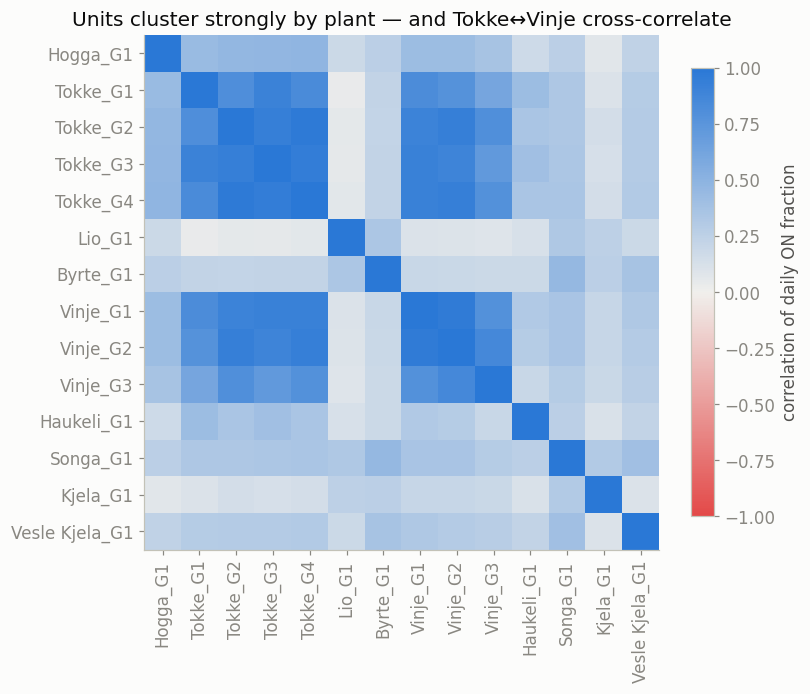
\includegraphics[width=\linewidth]{figures/eda_02_unit_correlation_heatmap.png}\end{subfigure}
\begin{subfigure}{0.49\linewidth}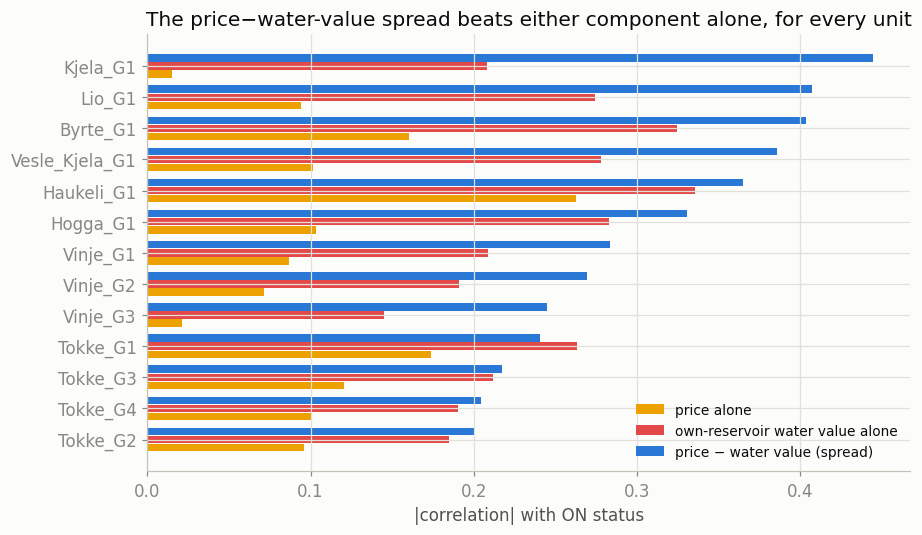
\includegraphics[width=\linewidth]{figures/eda2_05_spread_vs_components.png}\end{subfigure}
\caption{Left: correlation of units' daily on-fraction (blocks by plant; Tokke--Vinje coupled through
the cascade). Right: the price $-$ water-value spread correlates with commitment more strongly than
price or water value alone, for every unit. (Log 002, 008.)}
\label{fig:r-eda}
\end{figure}

% =============================================================================================
\section{Validation methodology}
\label{sec:r-val}

\paragraph{Random splits leak.} A random row split scores 0.957 with the same model that scores 0.835
on a held-out year: rows from one week are near-duplicates, and consecutive weeks share 144 hours at
88\% label agreement. Random \emph{case} splits still inflate by $+0.105$ (log 017). Every number in
this report therefore comes from a temporal split.

\paragraph{Walk-forward.} The reference protocol (logs 024, 028) has six half-year folds from 2020-H1
to 2022-H2; each trains on every case starting before the fold and scores the six months after.
Earlier stages used a single held-out year (2021, chosen as the most test-like year in log 020) or
four-fold rolling-origin CV; we judged changes on the per-fold sign pattern, since fold-to-fold
variation (SD up to 0.06) dwarfs most feature effects. A rotating-block scheme was built and
rejected: training on both sides of the held-out block measures interpolation, while the test set
requires extrapolation (log 035).

\paragraph{Which period resembles the test set?} We measured this instead of assuming it: a
classifier separates each half-year's cases from the 2023--24 test cases using case-level inputs
(price level, volatility, negative-price share, water value, spread, fill, inflow). 2021-H2 is the
hardest to separate (AUC 0.785), then 2022-H2 (0.879); every other half-year is above 0.95
(Figure~\ref{fig:r-adv}). We report these two \emph{test-like folds} separately. The test period
also contains negative prices in 2.2\% of hours, which the training data barely does.

\begin{figure}[H]
\centering
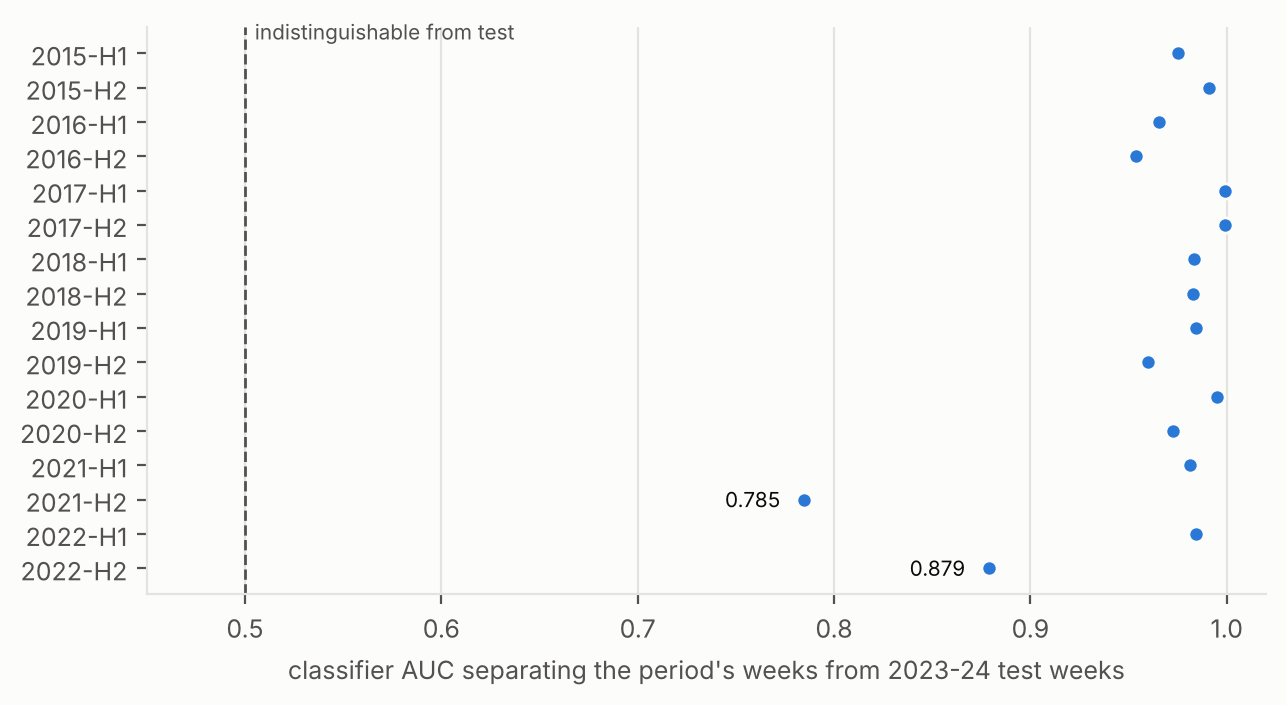
\includegraphics[width=0.72\linewidth]{figures/physics_06_adversarial.png}
\caption{Adversarial validation: how easily each half-year's cases are told apart from the test
cases. Lower is more test-like; 0.5 would be indistinguishable.}
\label{fig:r-adv}
\end{figure}

% =============================================================================================
\section{Track A: feature engineering for gradient-boosted trees}
\label{sec:r-fe}

Track A ran from a raw-feature baseline to our first submission over 36 logged sessions
(Appendix~\ref{app:log}). Table~\ref{tab:r-progress} lists the milestones; Table~\ref{tab:r-neg}
the main negative results.

\begin{table}[H]
\centering\small
\begin{tabular}{p{9.6cm}rl}
\toprule
step & micro-AUC & protocol \\
\midrule
14 independent XGBoost models, raw joined features & 0.647 & year 2022 \\
one multi-output tree (shared splits across units) & 0.687 & year 2022 \\
engineered features: spread $+0.075$, terminal water value $+0.034$ & 0.808 & 4-fold CV \\
pruned to 15 economic features (beats all 299) & 0.816 & 4-fold CV \\
\emph{oracle}: true hours-on per unit-week, allocated by spread rank & \emph{0.977} & year 2022 \\
count model as a budget augmentation of the pointwise model & 0.855 & year 2022 \\
water-balance (post-decision storage) features in the count model & 0.912 & year 2021 \\
distilled count outputs as features (compact architecture) & 0.935 & walk-forward \\
binned count head; hourly block structure & 0.944 & year 2021 \\
long format: one row per (case, hour, unit) & 0.950 & year 2021 \\
terminal water value read at start $+7$ days (documentation fix); tuning & 0.963 & year 2021 \\
\textbf{submitted model} (count model used only to rank features) & \textbf{0.9638} & walk-forward \\
\textbf{public leaderboard} & \textbf{0.98058} & test set \\
\bottomrule
\end{tabular}
\caption{Track A milestones. Protocols changed as the project matured, so rows are comparable only
within a protocol. Full table with all experiments: \texttt{report/leaderboard.md}.}
\label{tab:r-progress}
\end{table}

\paragraph{From raw features to economics (logs 004--015).} Independent per-unit models scored
0.647; one multi-output tree, letting correlated units share structure, 0.687. Twenty feature
themes were then built and screened. Nearly the whole gain came from two economic quantities, the
price $-$ water-value spread and the terminal water value; the strongest univariate correlate in
the project (a seasonal storage percentile, $+0.54$) made the model \emph{worse}. Pruning by gain
left 15 features, all economic, which beat the full 299.

\paragraph{The structural insight (log 018).} Given the true number of hours each unit is on in a
week, allocating them to the hours with the best spread already reaches 0.977. The hard part is
therefore \emph{one number per unit-week}, not which hours. A count model over hours-on, used first
as a logit augmentation and later distilled into features, carried the next $+0.10$.

\paragraph{Post-decision information (log 022).} The largest single jump ($+0.078$) came from
water-balance features built on the observed end-of-week storage. They are legal --- the volume file
covers the test period --- but they read the result of real-world operation rather than forecasting
it: without them the model scored 0.855. Track B removes this dependence.

\paragraph{Corrections, not inventions (logs 031--036).} The last gains were fixes: a graph
traversal that missed tunnel-fed plants ($+0.007$), the terminal water value read one day late
($+0.006$), the long format that made per-unit count features affordable ($+0.006$), hourly block
structure ($+0.003$), and \texttt{min\_child\_weight}$=500$ ($+0.002$; 6.9M rows but only
$\sim$100k independent blocks). Twelve further additions failed in a row (Table~\ref{tab:r-neg}).

\begin{table}[H]
\centering\small
\begin{tabular}{p{10cm}rl}
\toprule
rejected idea & effect & log \\
\midrule
expanding-window seasonal percentile (strongest univariate signal) & $-0.020$ & 013 \\
``physics'' stage (heads, MWh per m\textsuperscript{3}) as features & $-0.012$ & 014 \\
per-unit residual stage on top of the joint model & $+0.000$ & 016 \\
predict the count, then allocate hours by spread (hard) & $-0.055$ & 018 \\
corrected water balance for the four worst units & $-0.003$ & 027 \\
narrower, unit-resolved count model & $-0.029$ & 030 \\
one contiguous block per unit-week (oracle counts) & $-0.043$ & 031 \\
per-unit calibration, even with oracle base rates & $-0.005$ & 031 \\
67-year inflow climatology & $-0.000$ & 031 \\
min-flow obligation per plant & $-0.003$ & 031 \\
up-weighting the weakest unit (Lio) & $-0.001$ & 032 \\
287 slope (rate-of-change) features & $-0.002$ & 035 \\
full count distribution forwarded; hydraulic neighbour counts & $-0.001$ & 035 \\
\bottomrule
\end{tabular}
\caption{Track A negative results (single-year or stride-3 protocols). Kept as evidence: they
are why we concluded the feature set was saturated for that architecture.}
\label{tab:r-neg}
\end{table}

\paragraph{The submitted model} (Short notebook 2): one binary XGBoost model on one row per
(case, hour, unit), 6.87M rows and 207 features --- 15 pruned economic features, 35 terminal
water-value features, 36 hourly-structure features, 141 per-unit count-table features (chosen by a
6-class count model fitted only to rank them) and 5 static unit attributes; 600 rounds, depth 8,
learning rate 0.05, \texttt{min\_child\_weight} 500. Walk-forward 0.9638, public leaderboard 0.98058.
Lio (0.86) and Haukeli (0.92) remained weak, and predicted schedules switched 7.6 times a week
against 3.0 in reality.

% =============================================================================================
\section{Track B: rebuild the optimiser, learn only its errors}
\label{sec:r-lp}

\subsection{Motivation}

Track A approximated SHOP with features. But the labels are not noisy observations: they are the
output of one deterministic optimiser, and every input it used is in our data --- the topology file
is literally SHOP-ready. So we rebuilt the optimisation problem itself (\texttt{src/shoplite.py};
Short notebook 1, Sections 1--4).

\subsection{The model}

One linear programme per case, the LP relaxation of SHOP's weekly unit-commitment problem, solved
with HiGHS (dual simplex, $\sim$2\,s per case on one core; SHOP's own recorded solve times are a
median 52\,s, mean 147\,s):
\[
\max\ \sum_t \lambda_t \big(P_t - L_t\big) \;-\; \text{start/stop costs} \;-\; \text{river, bypass, spill costs}
\;-\; \text{penalties} \;+\; \sum_r \omega_r V_{r,T}
\]
subject to hourly water balance in all 17 reservoirs, the Vest-Vassdraget river junction and the
Songa tunnel junction; reservoir bounds; minimum volume and minimum flow (soft, heavily penalised);
for every unit an on/off variable $u\in[0,1]$ carrying the minimum block ($q_{\min}$, $p_{\min}$)
plus segments of the concave envelope of its PQ curve at the case's initial head (turbine efficiency
interpolated between the reference-head curves, times generator efficiency); start/stop variables
with the topology's costs; and main-tunnel and shared-penstock friction $L_t$ as a convex
piecewise-linear cubic in plant flow. $\lambda_t$ is the price and $\omega_r$ the terminal value of
water (below). The LP's duals give the hourly shadow price of water in each reservoir, from which
each unit's \emph{local water value} (EUR/MWh) and its margin, price $-$ local water value, follow.

Simplifications against SHOP, each a place the replica can disagree with the labels: heads frozen at
their initial levels (SHOP iterates), lossless tunnels between reservoirs, and an unknown initial
on/off state (we checked whether it chains from the previous case: hour 0 agrees with the previous
case's hour 24 only 80--96\% of the time, no more than overlapping cases agree in general).

\subsection{Three conventions measured from the labels}

The documentation does not say how SHOP turned the EUR/MWh water values into the value of a cubic
metre, how the river cost curves are read, or how identical units are ordered. Each was decided by
measurement:

\textbf{Terminal water value.} In weeks where a unit switches, its on-hour and off-hour prices
bracket the threshold SHOP used. Regressing that implied threshold on terminal water values gives
$\approx 1.0\times$ the feeding reservoir's value and $\approx 0\times$ the downstream value
(Figure~\ref{fig:r-thr}; Byrte slope 0.98, $R^2$ 0.99). The textbook conversion --- EUR/MWh times the
full-cascade energy-conversion factor --- predicts a large negative downstream coefficient and is
refuted. The convention that reproduces the labels values one Mm\textsuperscript{3} in reservoir
$r$ as $\omega_r=\sum_k \mathrm{WV}(\text{reservoir feeding }k)\cdot \mathrm{conv}_k$ over the
plants $k$ on its way to the sea, so each plant breaks even exactly at its own reservoir's value.

\textbf{River flow cost.} Reading \texttt{flow\_cost\_curve} as a marginal cost per
(m\textsuperscript{3}/s$\cdot$h) charged Kjela's discharge 33 EUR on its way through
\texttt{r\_Hyljelihyl} --- the LP duals showed exactly that gap. Read as total cost per hour (marginal
cost = slope), Kjela's raw AUC rose from 0.70 to 0.96 and Haukeli's from 0.93 to 0.99.

\textbf{Sibling order.} The merit order measured in EDA, stable in every year, is imposed as
$u_{\text{G1}}\ge u_{\text{G3}}\ge u_{\text{G4}}\ge u_{\text{G2}}$ at Tokke and
$u_{\text{G1}}\ge u_{\text{G2}}\ge u_{\text{G3}}$ at Vinje: ``which unit'' becomes ``how many''.

On a 59-case sample across all years the raw LP's micro-AUC went 0.937 $\to$ 0.963 (river cost)
$\to$ 0.967 (sibling order), with no training data.

\begin{figure}[H]
\centering
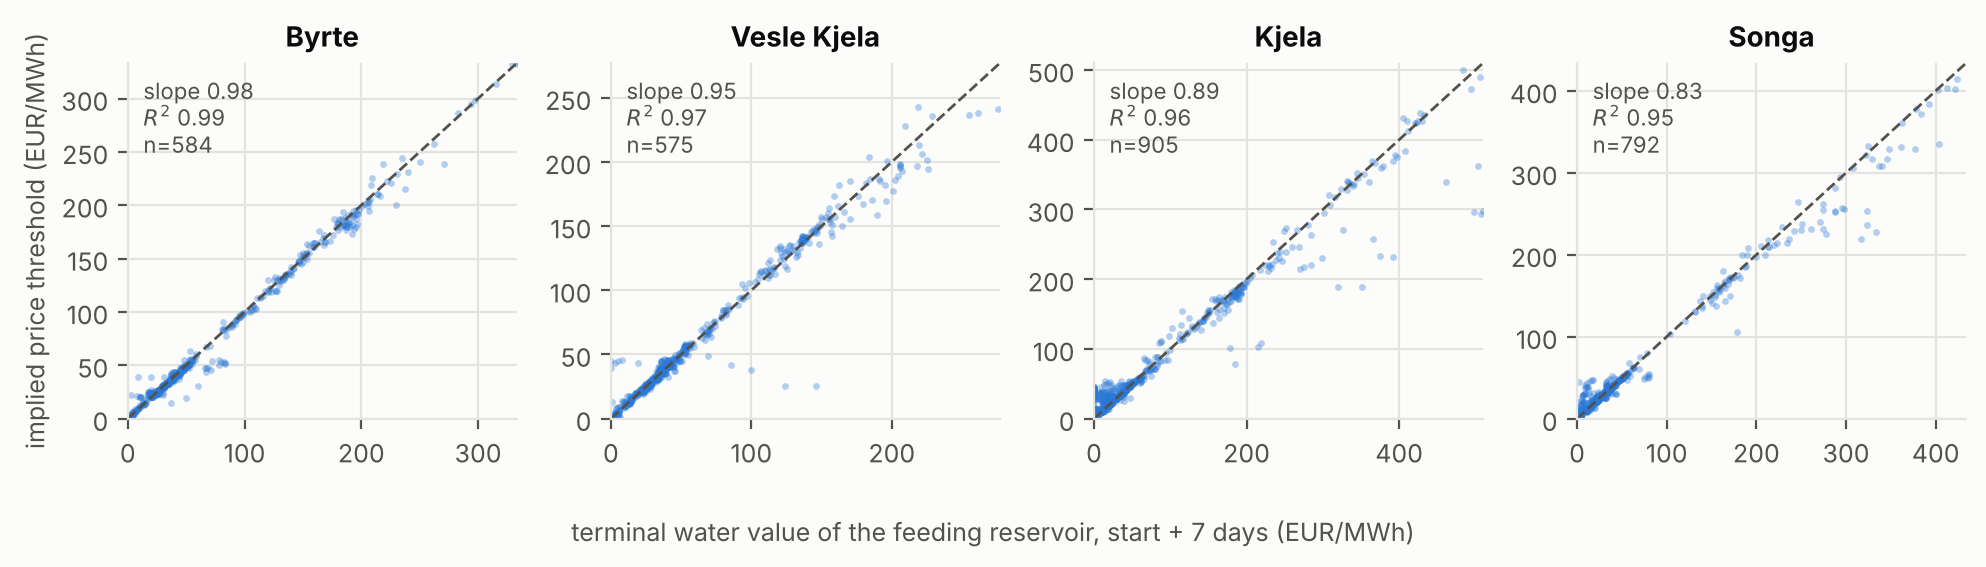
\includegraphics[width=\linewidth]{figures/physics_01_threshold_vs_water_value.png}
\caption{Implied price threshold in every mixed week against the terminal water value of the
reservoir feeding the plant. Points lie on $y=x$: each plant breaks even at its own reservoir's
water value, whatever the downstream values are.}
\label{fig:r-thr}
\end{figure}

\paragraph{The MILP is a worse feature than the LP.} Solving with binary $u$ scored 0.941 against the
LP's 0.967 on the same sample: a 0/1 schedule loses the graded information about how close each hour
is to the margin, and a small model error flips a whole block. It also exposed a genuine gap: SHOP
keeps Lio on all week to meet the Vest-Vassdraget minimum flow even when price is below its
reservoir's water value, while our MILP pulses Lio and bypasses Vinjevatn instead. Gaps like this are
what the learned layer corrects.

\subsection{The learned correction}

LightGBM on one row per (case, hour, unit), 61 features (Short notebook 1, Section 5):
\texttt{lp\_} --- the LP solution (commitment, power, flow), its temporal context (rolling windows,
run lengths, weekly and daily means, plant-level number of units on), the local water value and
margin, and the reservoir trajectories; \texttt{ec\_} --- price level, rank and z-score within the
week, spread to the terminal water value, season, inflow; \texttt{cn\_} --- the constraint series;
\texttt{st\_} --- the observed storage trajectory; \texttt{s\_} --- unit identity and static
attributes. 600 rounds, learning rate 0.05, 127 leaves, \texttt{min\_data\_in\_leaf} 500.

\subsection{Results}

Both tracks were run on the same six walk-forward folds on the same machine, each training on
every third case (the project's experiment convention); the submitted XGBoost model re-run this way
reproduces its recorded 0.9638 to within 0.002.

\begin{table}[H]
\centering\small
\begin{tabular}{lrrrr}
\toprule
fold & XGBoost (Track A) & raw LP, no learning & LP + LightGBM & $\Delta$ \\
\midrule
2020-H1 & 0.9535 & 0.9720 & \textbf{0.9925} & $+0.039$ \\
2020-H2 & 0.9455 & 0.9671 & \textbf{0.9866} & $+0.041$ \\
2021-H1 & 0.9765 & 0.9787 & \textbf{0.9950} & $+0.019$ \\
2021-H2 (test-like) & 0.9504 & 0.9695 & \textbf{0.9914} & $+0.041$ \\
2022-H1 & 0.9672 & 0.9586 & \textbf{0.9862} & $+0.019$ \\
2022-H2 (test-like) & 0.9784 & 0.9802 & \textbf{0.9953} & $+0.017$ \\
\midrule
mean (SD) & 0.9619 (0.014) & 0.9710 (0.008) & \textbf{0.9912 (0.004)} & $+0.029$ \\
\bottomrule
\end{tabular}
\caption{Walk-forward micro ROC-AUC.}
\label{tab:r-wf}
\end{table}

\begin{figure}[H]
\centering
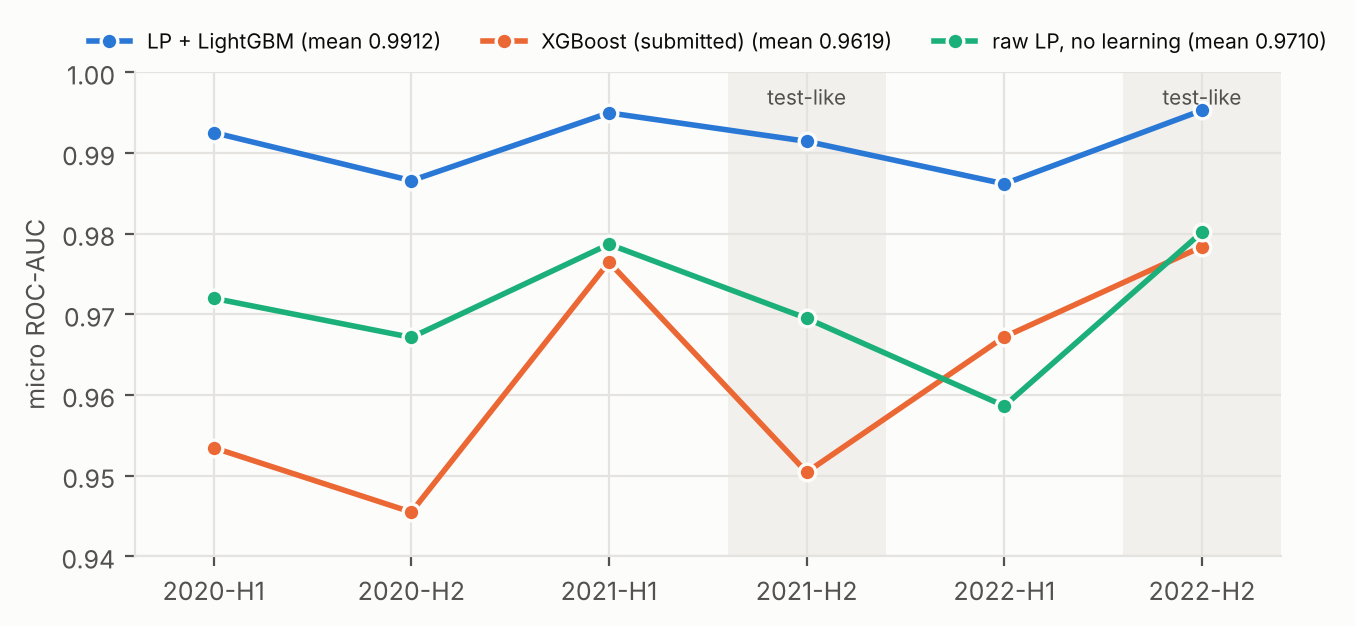
\includegraphics[width=0.85\linewidth]{figures/physics_02_walkforward.png}
\caption{Walk-forward results per fold. The raw optimiser, which uses no labels, beats the trained
XGBoost model on five of six folds.}
\label{fig:r-wf}
\end{figure}

Every fold and every unit improves (Figure~\ref{fig:r-unit}); the two units Track A never fixed move
most (Lio 0.864 $\to$ 0.979, Haukeli 0.920 $\to$ 0.973), and the fold SD falls from 0.014 to 0.004.
Trained on all 2{,}922 cases, the model scores \kagglelp{} on the public leaderboard.

\begin{figure}[H]
\centering
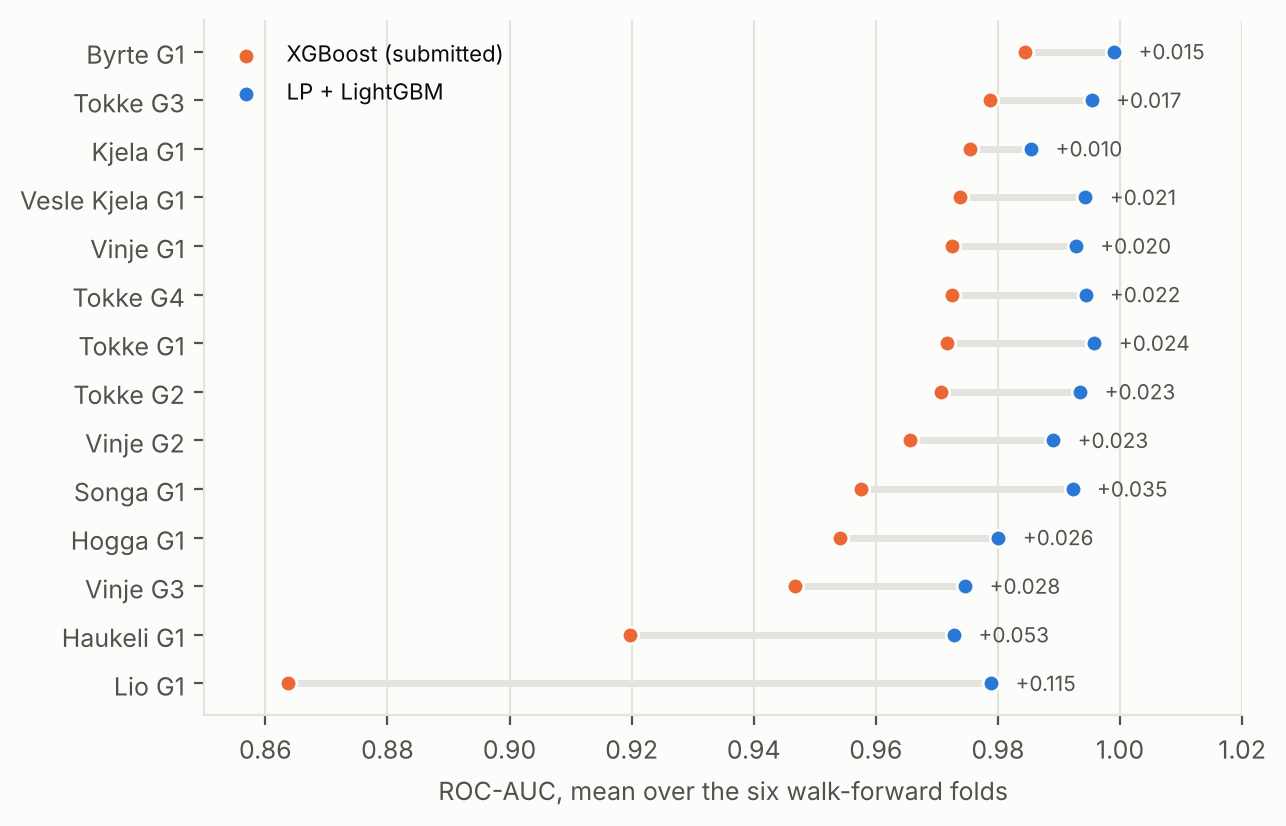
\includegraphics[width=0.75\linewidth]{figures/physics_03_per_unit.png}
\caption{Per-unit ROC-AUC, mean over the six folds, Track A (orange) and Track B (blue).}
\label{fig:r-unit}
\end{figure}

% =============================================================================================
\section{Model interpretation}
\label{sec:r-interp}

\subsection{Track A: what the trees learned}

The pruned 15 features are all economic quantities --- spreads, margins, break-even hours, the
share of capacity a spread justifies --- with topology used only to pick \emph{which} water value
and \emph{which} capacity; no raw price, storage, inflow or calendar column survived (log 017). The
single most important feature of the early model, by a factor of 14, was the binary
``price $>$ system water value'': SHOP's dispatch condition, rediscovered
(Figure~\ref{fig:r-imp-a}). In the count model the top feature was the system storage change over
the week --- released water, i.e.\ production --- and the binding-constraint term
$\min(\text{hours of water}, \text{hours profitable})$ (logs 021--022). Hourly-varying features
held 96\% of the gain: micro-AUC rewards ranking hours \emph{within} a week, which a case-level
constant cannot do (log 013).

\begin{figure}[H]
\centering
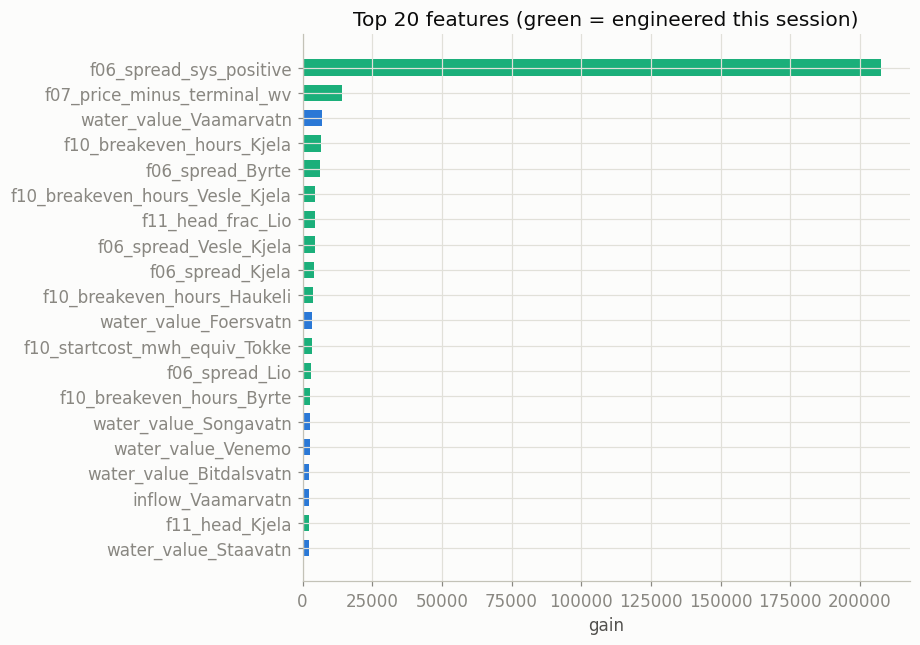
\includegraphics[width=0.62\linewidth]{figures/iter1_02_feature_importance.png}
\caption{Track A, first feature iteration: gain importance. The binary spread sign --- SHOP's own
dispatch condition --- dominates. (Log 013.)}
\label{fig:r-imp-a}
\end{figure}

\subsection{Track B: the model leans on the optimiser}

\paragraph{Ablation.} Removing one feature group at a time on the same folds
(Figure~\ref{fig:r-abl}): without the LP features the same learner scores 0.9483 --- \emph{below}
Track A --- so the gain is neither LightGBM nor the feature engineering. The LP features plus unit
identity alone reach 0.9897. Removing the observed storage trajectory changes nothing (0.9910 vs
0.9912): the model uses only information available before the week starts, unlike Track A's best
features.

\begin{figure}[H]
\centering
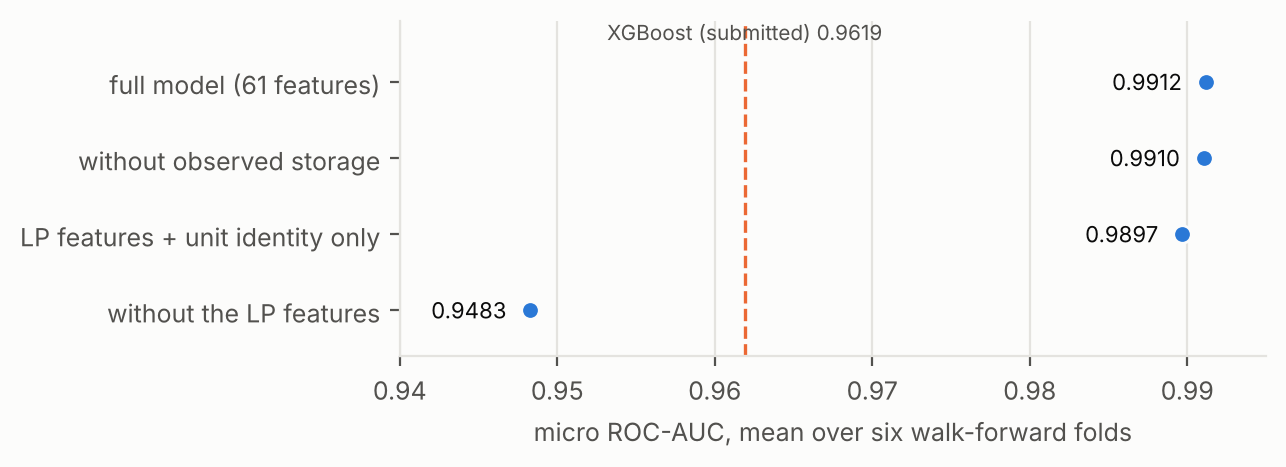
\includegraphics[width=0.72\linewidth]{figures/physics_04_ablation.png}
\caption{Ablation: mean walk-forward micro-AUC with one feature group removed.}
\label{fig:r-abl}
\end{figure}

\paragraph{Importance.} The LP commitment and flow alone carry 71\% of the split gain, LP features
86\% in total (Figure~\ref{fig:r-gain}). Unit identity (5\%) is how the model learns per-unit
corrections --- e.g.\ that SHOP runs Lio harder than our LP does.

\begin{figure}[H]
\centering
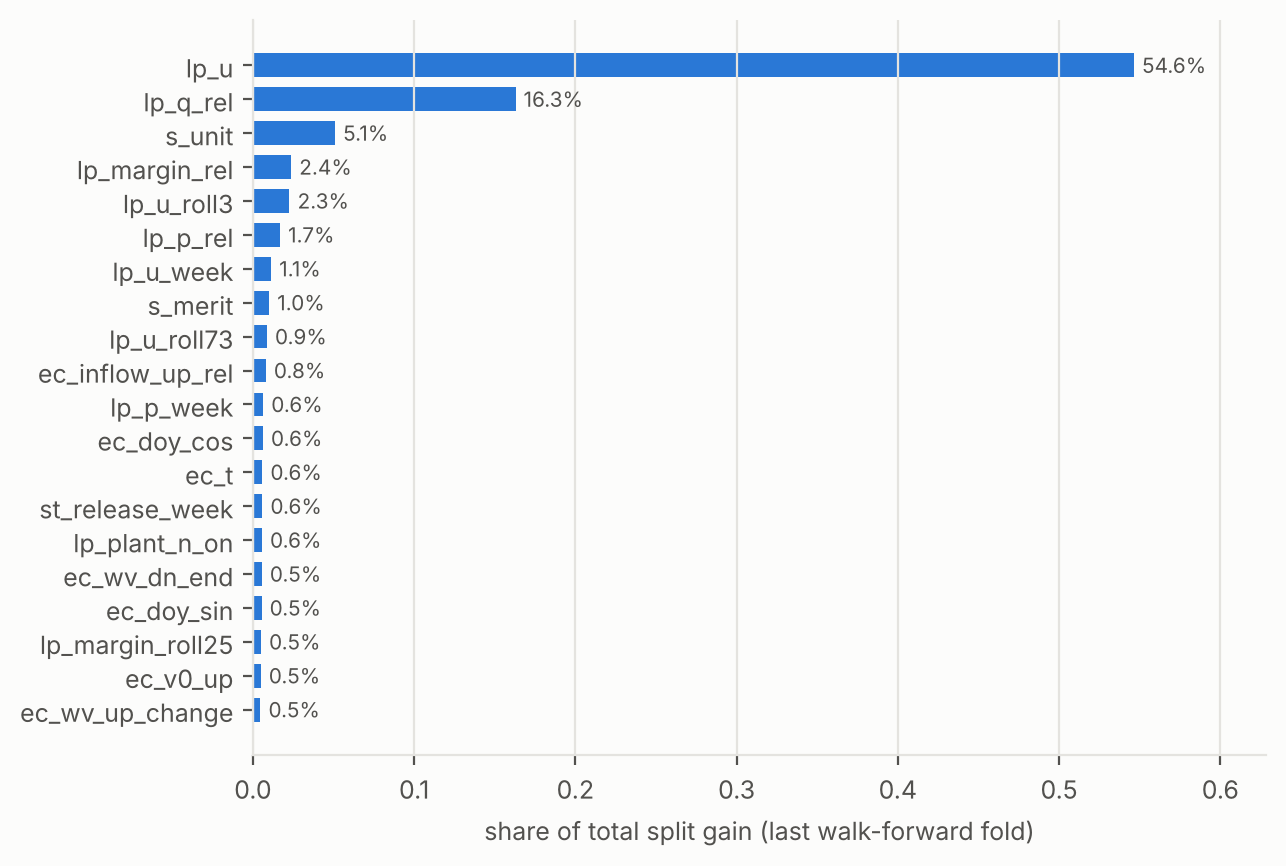
\includegraphics[width=0.62\linewidth]{figures/physics_05_gain_importance.png}
\caption{LP + LightGBM: share of split gain, top 20 features (last walk-forward fold).}
\label{fig:r-gain}
\end{figure}

\paragraph{Contributions.} Split gain counts how much a feature is used in training, not how much it
moves a prediction. TreeSHAP contributions (LightGBM's \texttt{pred\_contrib}) on 20{,}000 validation
rows of the test-like 2021-H2 fold (fold AUC 0.9914) give the per-prediction view
(Figure~\ref{fig:r-contrib}). The LP commitment $u$ moves the log-odds by 2.05 on average, nearly
twice any other feature. Unit identity is second (1.14): it is the channel for per-unit corrections.
Third is the margin, price minus the local water value from the LP duals (0.93), with its 7-hour
rolling mean close behind: the learner reads how far each hour sits from the dispatch threshold,
exactly the graded information a binary schedule discards (Section~\ref{sec:r-lp}). By group, LP
features carry 70\% of the total absolute contribution, economics 15\%, unit identity and static
attributes 13\%, the observed storage trace 2\% and the constraint series 1\%. Economics weigh more
here than in split gain (15\% against 6\% of the gain in the last fold): many small adjustments
rather than a few decisive splits.

\begin{figure}[H]
\centering
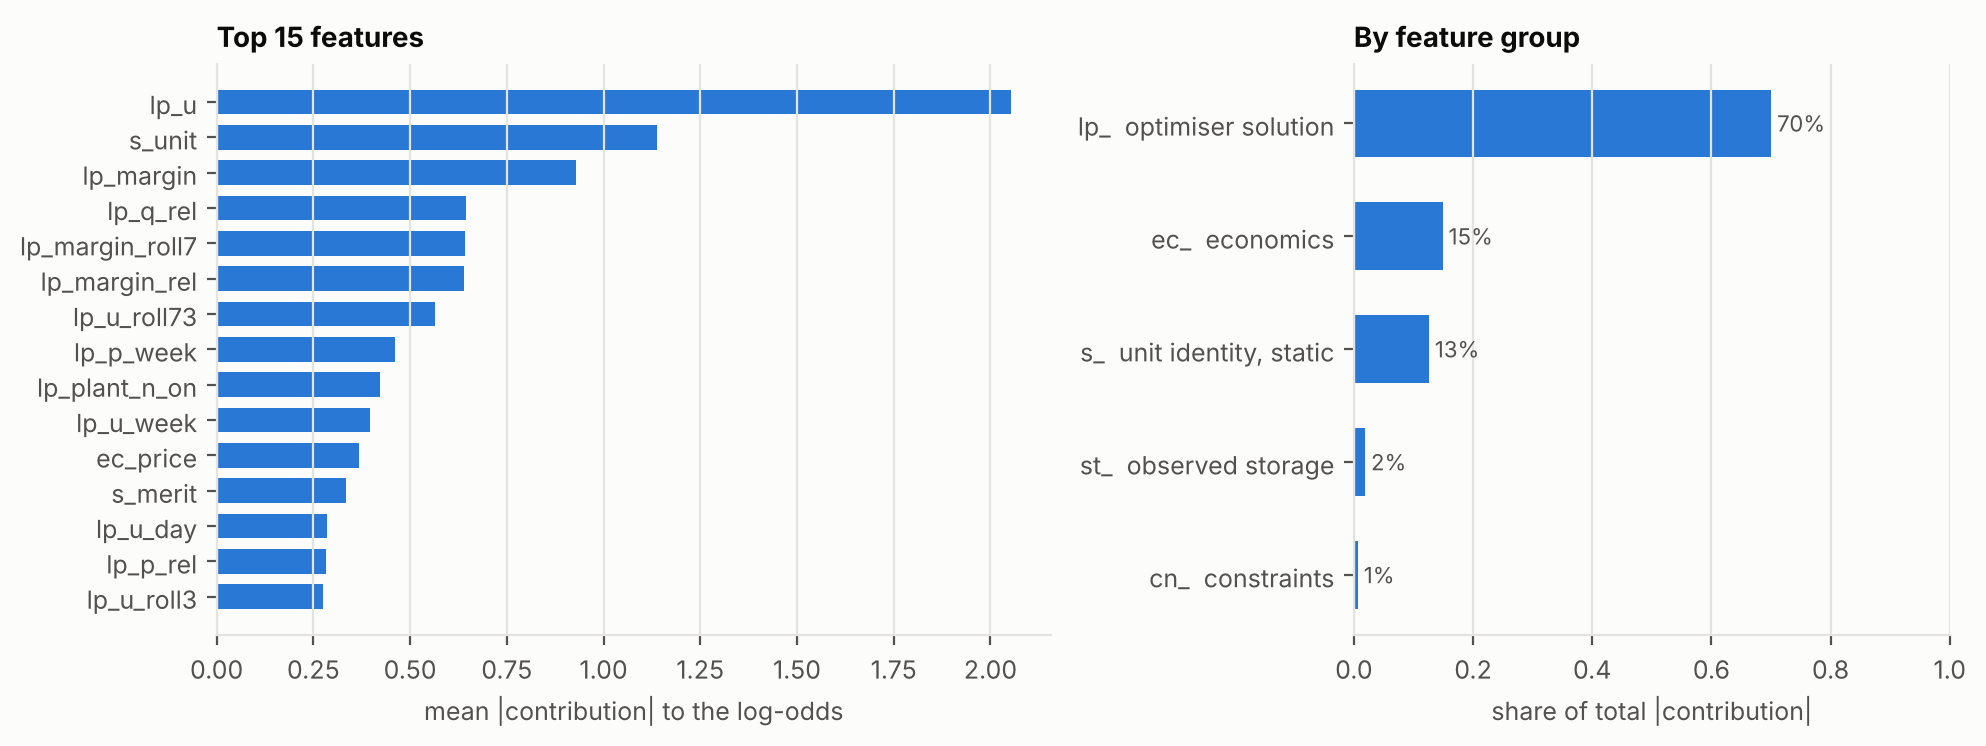
\includegraphics[width=0.95\linewidth]{figures/physics_07_contributions.png}
\caption{LP + LightGBM, 2021-H2 fold: mean absolute TreeSHAP contribution to the log-odds, top 15
features (left) and share by feature group (right).}
\label{fig:r-contrib}
\end{figure}

\paragraph{How the learned layer reads the LP.} The relaxation's $u$ is already roughly a probability
(Figure~\ref{fig:r-lpshop}): SHOP commits in about 1\% of hours where $u=0$ and 94\% where $u=1$, and the
on-rate rises close to the diagonal in between. The departures are unit-specific, which is why unit
identity ranks second. Lio, which SHOP runs to meet the Vest-Vassdraget minimum flow, is committed
in every hour where the LP gives it $u \geq 0.6$ and in three quarters of hours at $0.4$--$0.6$. Hogga,
whose timing is degenerate in our LP when Bandak must fill, is committed in only 45\% of hours at
$u$ between 0.6 and 0.8.

\begin{figure}[H]
\centering
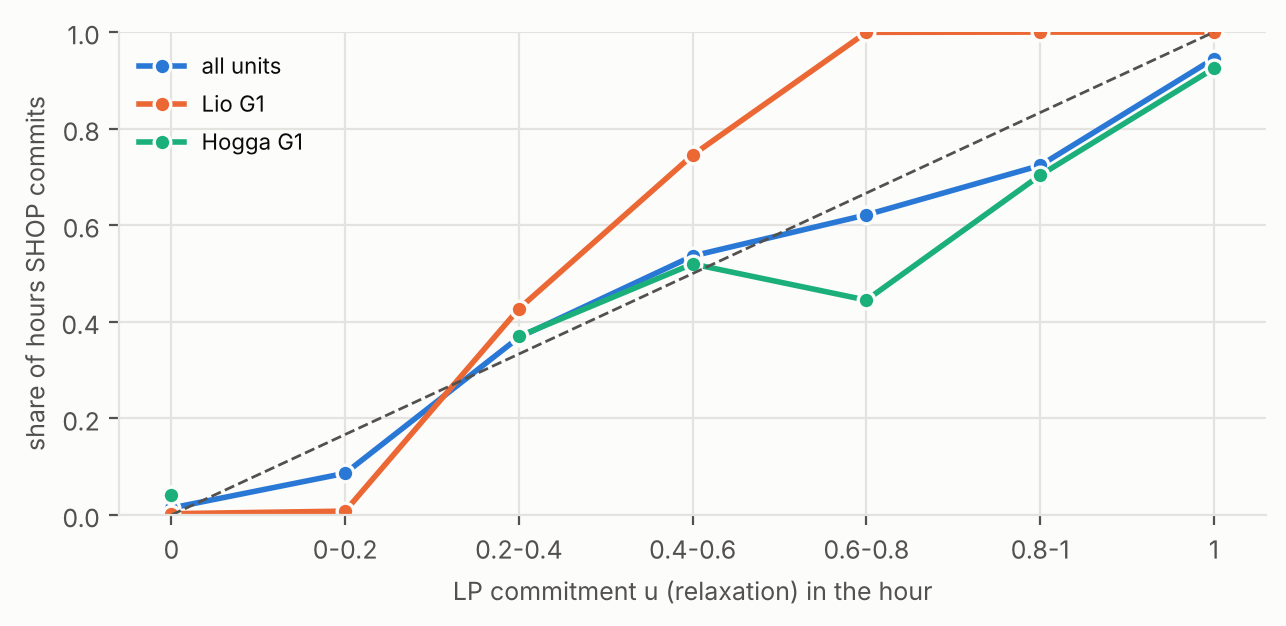
\includegraphics[width=0.68\linewidth]{figures/physics_08_lp_vs_shop.png}
\caption{Share of hours SHOP commits, by the LP relaxation's $u$ in that hour (2021-H2 fold). Dashed:
perfect calibration.}
\label{fig:r-lpshop}
\end{figure}

\paragraph{One week.} Figure~\ref{fig:r-week} shows a test-like case the LP finds harder than three
quarters of its fold. The relaxation spreads Tokke's commitment fractionally over four identical
units and holds Lio at $u \approx 0.45$ until day 3.5. The learned layer concentrates Tokke on G1, the
unit SHOP picks first, and sharpens Lio into the on-block SHOP chose; its within-case AUC is 0.999
against the LP's 0.974. Its remaining error is inherited from the LP: Kjela, on all week in SHOP's
schedule, dips where the relaxation dips (days 4.4--5.6).

\begin{figure}[H]
\centering
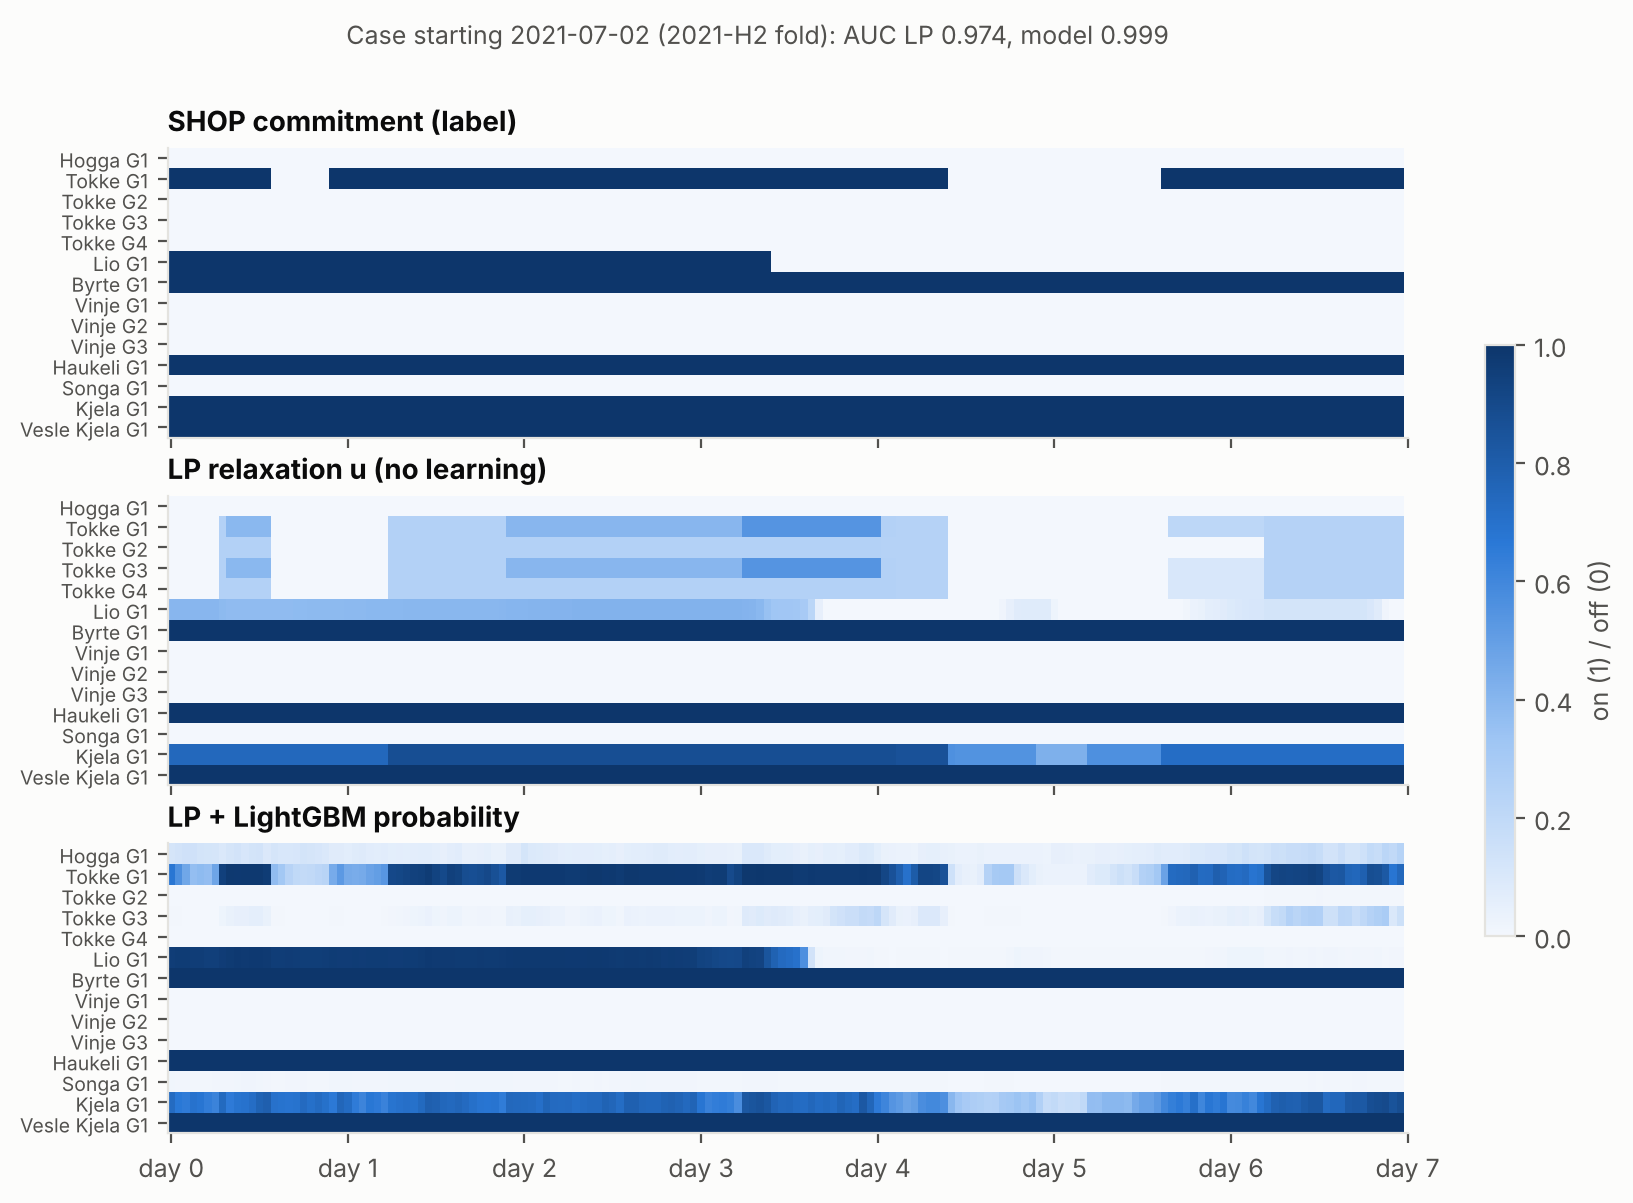
\includegraphics[width=0.86\linewidth]{figures/physics_09_example_week.png}
\caption{Case starting 2021-07-02: SHOP's commitment (top), the LP relaxation with no learning
(middle) and the LP + LightGBM probability (bottom), one row per unit, one column per hour.}
\label{fig:r-week}
\end{figure}


\paragraph{The optimiser itself is interpretable.} Its decisions are explained by quantities with
physical meaning: each unit runs when the price exceeds its local water value, which equals its
reservoir's terminal water value unless a constraint binds --- a full reservoir lowers it (water
would otherwise spill), a minimum-flow obligation can force a unit on below it, an empty reservoir
raises it. The three conventions of Section~\ref{sec:r-lp} are themselves findings about how the
labels were produced.

% =============================================================================================
\section{Discussion}
\label{sec:r-disc}

\paragraph{Why Track B works.} Track A spent most of its effort recovering, through features, a
decision process that is written down: the spread is the dispatch condition, the count is the
weekly water budget, the block structure comes from start costs, the merit order from penstocks.
Solving the actual problem gets all of these at once, consistently across units and reservoirs,
and extrapolates to unseen price regimes (negative prices, the post-crisis level) from physics
rather than from training data. The learner is left with a smaller, more stationary job: the
residual between our simplified replica and SHOP.

\paragraph{Relation to the task's purpose.} InterOpt wants ML to speed up the optimiser. Our best
model still solves an LP, but one $\sim$25--70$\times$ cheaper than SHOP, and its output is a
calibrated commitment probability that could warm-start SHOP's MIP. Unlike Track A's best
features, it needs no post-decision information.

\paragraph{Limitations and next steps.} The remaining errors are fidelity gaps of the replica: heads
frozen at their initial level, Lio's min-flow behaviour, weeks where SHOP runs units below their
water value (e.g.\ 2019-07-09), and degenerate weeks where a reservoir must fill and the timing of
release is arbitrary. Each fix to the replica feeds the learned layer directly. Three conventions
were read off label statistics that include the validation years; they are structural and stable
across years, but the protocol is not blind to them.

\paragraph{What we would do differently.} Read the topology file on day one. Track A's three
largest late gains were corrections found by reading the documentation; Track B is the same lesson
taken to its conclusion.

% =============================================================================================
\appendix
\section{Reproducibility}
\label{app:repro}

\begin{itemize}
\item \textbf{Short notebook 1} (LP + LightGBM): solves the 3{,}647 LPs in parallel ($\sim$1.6\,h on 4
  cores, cached after the first run), builds features, trains on all labelled cases and writes the
  submission ($\sim$10\,min, $\sim$6\,GB RAM). Verified to reproduce the uploaded file to $2\cdot
  10^{-13}$; the notebook's LP code reproduces the stored solutions bit for bit.
\item \textbf{Short notebook 2} (XGBoost): builds the hourly table from the raw files, the feature
  stages, the count table and model, the hourly structure and the long format, and trains on all
  labelled cases (about 45\,min and $\sim$20\,GB of memory including swap on 4 cores). The long design matrix is assembled in place instead of through
  pandas concatenations; it is verified identical to the original assembly, value for value. The
  uploaded file was produced on an Apple Silicon Mac. On x86 Linux with the same package versions
  the count model's importance ranking selects 143 count features instead of 141 (identically at 4
  and 8 threads, so not a threading effect), and the output correlates 0.995 with the uploaded file,
  with 98\% of cells on the same side of 0.5. We attribute this to platform-level floating-point
  differences that reorder near-tied features; the notebook's last cell reports the comparison.
\item Source modules, every experiment and its result: \texttt{src/}, \texttt{report/leaderboard.md},
  \texttt{report/runs/}.
\end{itemize}

\section{Full lab log}
\label{app:log}

The chronological record of every session, including all experiments and negative results, exactly
as written during the project.
\sloppy

\renewcommand{\thesubsection}{B.\arabic{subsection}}
\subsection{2026-09-21 --- Problem framing and data overview}

\subsubsection*{Task.} SINTEF Energy's InterOpt project: predict, for each of 14 generating units in
the Tokke--Vinje hydropower system (17 reservoirs, 9 plants, southern Norway), the probability
that the unit is ON at every hour of a 168-hour (one-week) rolling scheduling horizon. Ground
truth comes from a SHOP optimization run. Submissions are scored on Kaggle with
\textbf{micro-average ROC-AUC}. The intent (per the task PDF) is for a trained ML model to
approximate what the optimizer would decide, to speed up real hydropower scheduling.

\subsubsection*{Case structure.} The full problem spans 3{,}647 daily rolling cases
(2015-01-01 to 2024-12-25). Labels only exist for the first 2{,}922 cases
(2015-01-01 to 2022-12-31, \texttt{data/kernel/Unit\_commitment\_decisions.csv}); the remaining
725 cases (2023-01-01 to 2024-12-25, \texttt{prediction\_mapping.csv}) are the held-out Kaggle
test set.

\subsubsection*{Data layout.} Two source folders, kept as raw, unmodified files (see
Section~\ref{sec:modeling-table} for why we don't leave them scattered when actually modeling):

\begin{itemize}
  \item \texttt{data/kernel/} (core, required): hourly day-ahead price, hourly reservoir/river
    inflow (17 reservoirs + 1 river), daily reservoir storage, daily marginal water value,
    and the ground-truth unit commitment decisions.
  \item \texttt{data/extended/} (optional context): watercourse topology
    (\texttt{Tokke\_Vinje\_topology.yaml}, SHOP-format graph of reservoirs / rivers / tunnels /
    plants / generators), a topology diagram PDF, and hourly environmental constraints (minimum
    reservoir volume, minimum river flow).
\end{itemize}

\finding{No missing values in any core or extended file; reservoir naming is consistent across
files; \texttt{Constraint\_min\_volume}/\texttt{min\_flow} reservoirs/rivers are a strict subset
of the full 17. The data is clean going in.}

\finding{\texttt{total\_calculation\_time} (SHOP solver runtime) is present in the training
labels file but is solver metadata, not a feature --- it does not exist for the test cases we
need to predict. It must be excluded from any feature pipeline to avoid leakage.}

\subsection{2026-09-21 --- Exploratory data analysis}
\label{sec:eda}

Full notebook: \texttt{src/EDA/eda.ipynb}. Figures below are extracted from its executed
outputs; see \texttt{figures.md} for exact provenance per figure.

\subsubsection*{Target: per-unit imbalance and correlation structure.}

\begin{figure}[htbp]
  \centering
  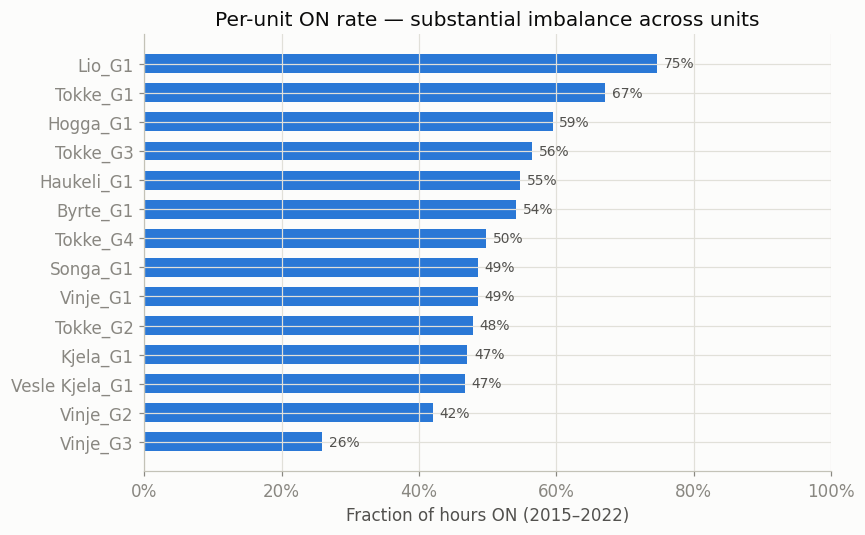
\includegraphics[width=0.75\linewidth]{figures/eda_01_unit_on_rate.png}
  \caption{Per-unit ON rate, 2015--2022.}
  \label{fig:eda-unit-on-rate}
\end{figure}

\finding{ON rate varies from 26\% (Vinje\_G3) to 75\% (Lio\_G1) across units
(Figure~\ref{fig:eda-unit-on-rate}) --- this is not one balanced binary problem, and per-unit
performance should be tracked separately, not just the pooled micro-AUC.}

\begin{figure}[htbp]
  \centering
  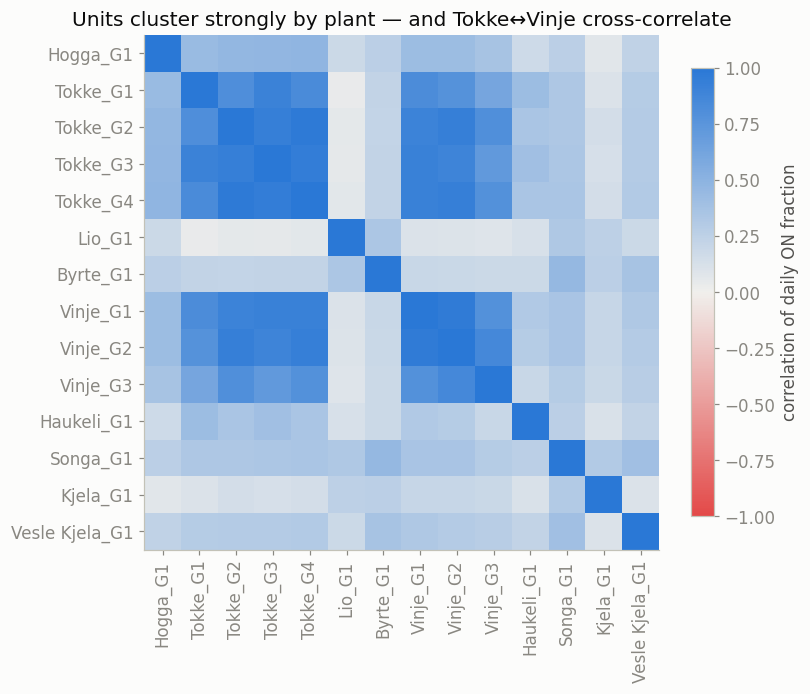
\includegraphics[width=0.75\linewidth]{figures/eda_02_unit_correlation_heatmap.png}
  \caption{Correlation of units' daily ON fraction, ordered by plant.}
  \label{fig:eda-unit-corr}
\end{figure}

\finding{Units at the same plant correlate strongly (0.8--0.96). More notably, Tokke and Vinje
--- different plants, different immediate reservoirs --- also cross-correlate at 0.8--0.9
(Figure~\ref{fig:eda-unit-corr}). This turned out to be explainable by the watercourse
topology: Vinje's reservoir (Vaamarvatn) cascades downstream into Vinjevatn, which is exactly
the reservoir Tokke draws from. This motivates modeling units jointly rather than as 14
independent problems.}

\subsubsection*{Seasonality.}

\begin{figure}[htbp]
  \centering
  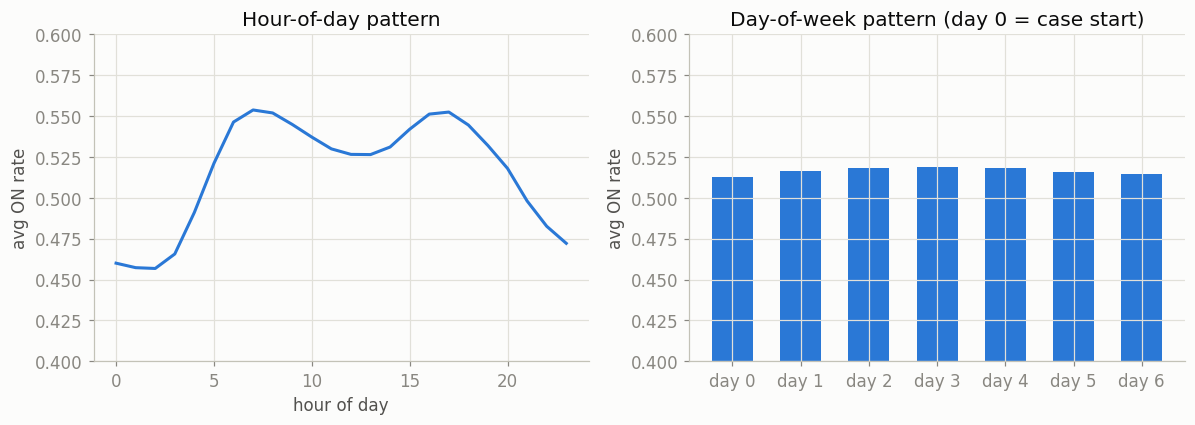
\includegraphics[width=0.95\linewidth]{figures/eda_03_hour_and_dow_pattern.png}
  \caption{ON rate by hour-of-day and by day-of-week within a case.}
  \label{fig:eda-hod-dow}
\end{figure}

\finding{Strong intraday seasonality (double-hump pattern, trough $\approx$0.46 at night,
peaks $\approx$0.55 at the morning/evening demand ramps) but weak day-of-week seasonality
(0.51--0.52 across all 7 days) --- see Figure~\ref{fig:eda-hod-dow}. \texttt{hour\_of\_day} is a
much more informative time feature than \texttt{day\_of\_week} here.}

\subsubsection*{Yearly trend and the 2022 outlier.}

\begin{figure}[htbp]
  \centering
  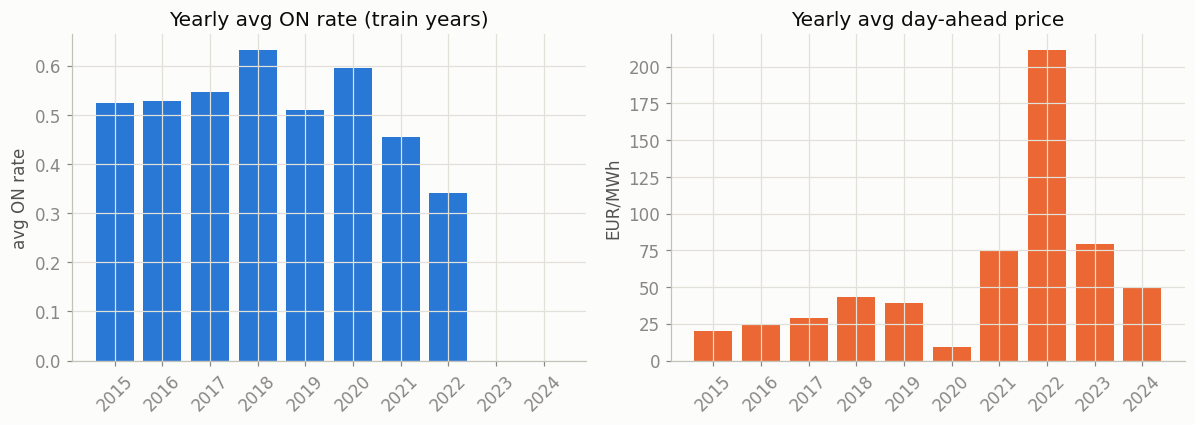
\includegraphics[width=0.75\linewidth]{figures/eda_04_yearly_on_rate_vs_price.png}
  \caption{Yearly average ON rate vs.\ yearly average day-ahead price.}
  \label{fig:eda-yearly}
\end{figure}

\begin{figure}[htbp]
  \centering
  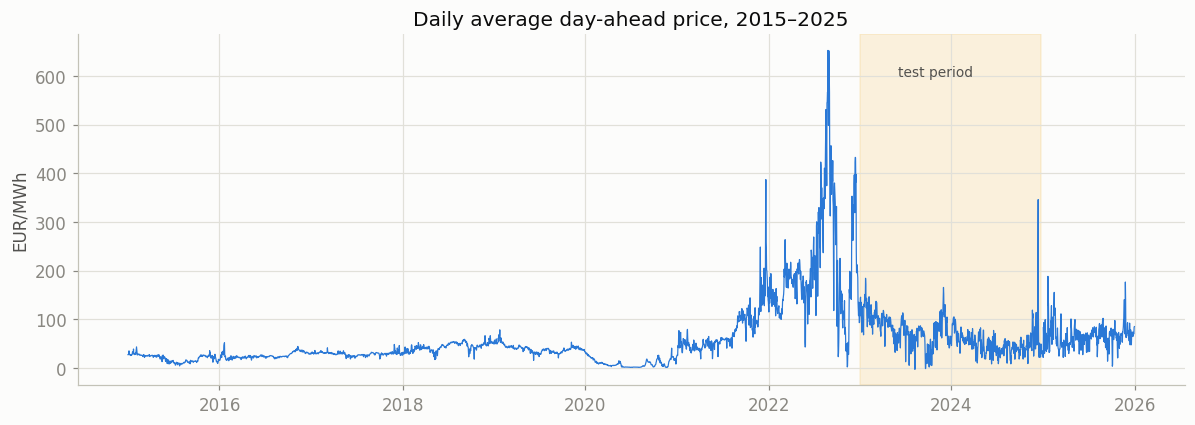
\includegraphics[width=0.85\linewidth]{figures/eda_05_price_timeseries.png}
  \caption{Daily average price, 2015--2025, with the 2023--2024 test window shaded.}
  \label{fig:eda-price-ts}
\end{figure}

\finding{2022 (European energy crisis) has the \emph{highest} average price in the series
($\sim$211 EUR/MWh) but the \emph{lowest} average ON rate (0.34) --- see
Figure~\ref{fig:eda-yearly}. The naive ``high price $\Rightarrow$ more generation'' intuition
does not hold at the year level (explained further below). The 2022 spike sits entirely in the
training window; the test window (2023--2024, shaded in Figure~\ref{fig:eda-price-ts}) is
elevated relative to 2015--2020 but nowhere near the 2022 extreme --- a distribution-shift risk
that motivated a chronological (not random) validation split for modeling.}

\subsubsection*{Physical drivers: inflow, storage, water value.}

\begin{figure}[htbp]
  \centering
  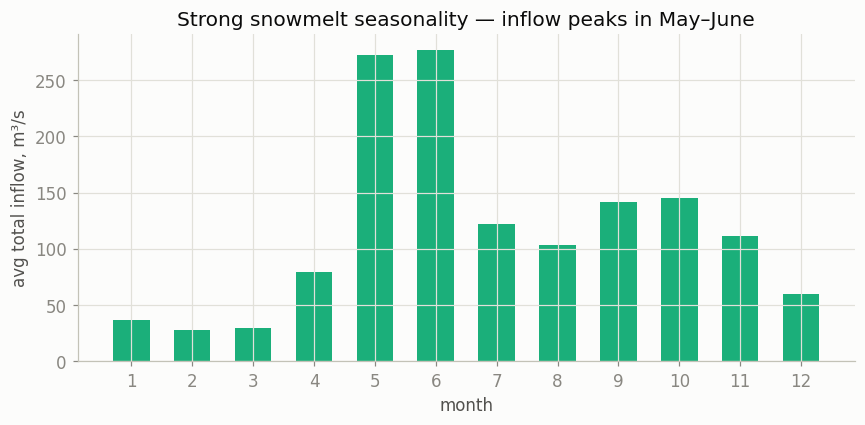
\includegraphics[width=0.7\linewidth]{figures/eda_06_inflow_seasonality.png}
  \caption{Average total reservoir inflow by calendar month.}
  \label{fig:eda-inflow-season}
\end{figure}

\begin{figure}[htbp]
  \centering
  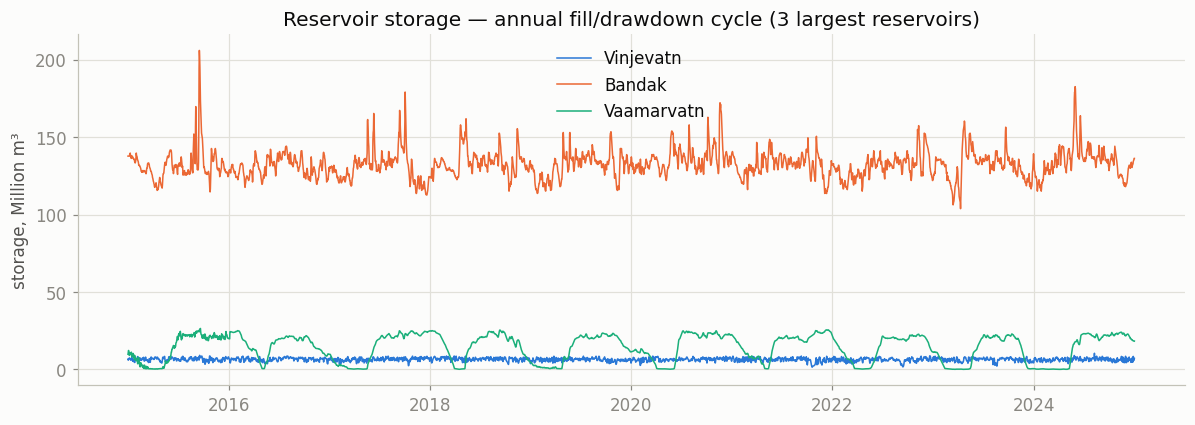
\includegraphics[width=0.85\linewidth]{figures/eda_07_reservoir_storage_cycle.png}
  \caption{Daily storage, three largest reservoirs.}
  \label{fig:eda-storage}
\end{figure}

\begin{figure}[htbp]
  \centering
  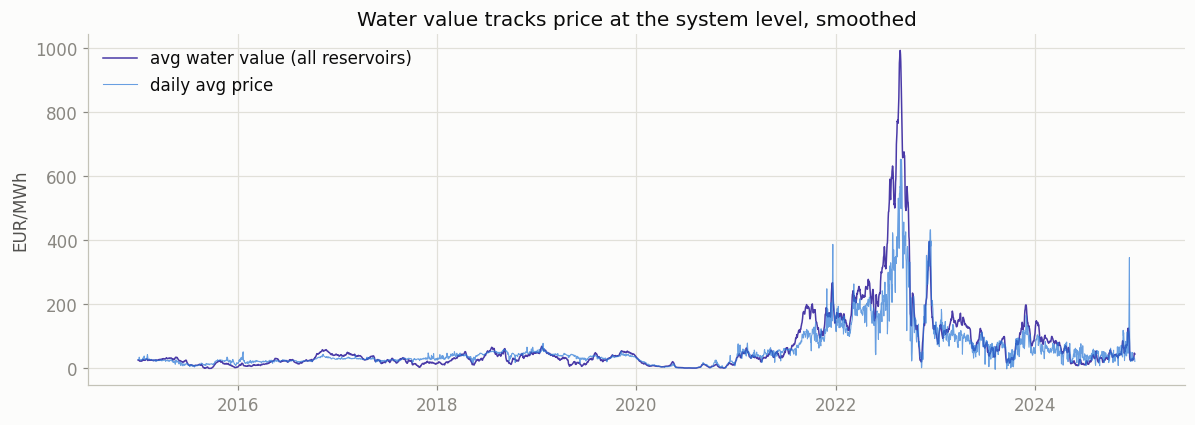
\includegraphics[width=0.85\linewidth]{figures/eda_08_water_value_vs_price.png}
  \caption{System-average water value vs.\ daily average price.}
  \label{fig:eda-wv-price}
\end{figure}

\finding{Classic Norwegian snowmelt seasonality: total inflow across all 17 reservoirs is
$\sim$8$\times$ higher in May--June than in the Jan--Feb trough
(Figure~\ref{fig:eda-inflow-season}), driving the annual storage fill/drawdown cycle
(Figure~\ref{fig:eda-storage}). System-average water value tracks price but is much smoother
(Figure~\ref{fig:eda-wv-price}) --- it reflects the expected \emph{future} value of stored
water, not the instantaneous spot price.}

\subsubsection*{The headline finding: relative price, not absolute price.}

\begin{figure}[htbp]
  \centering
  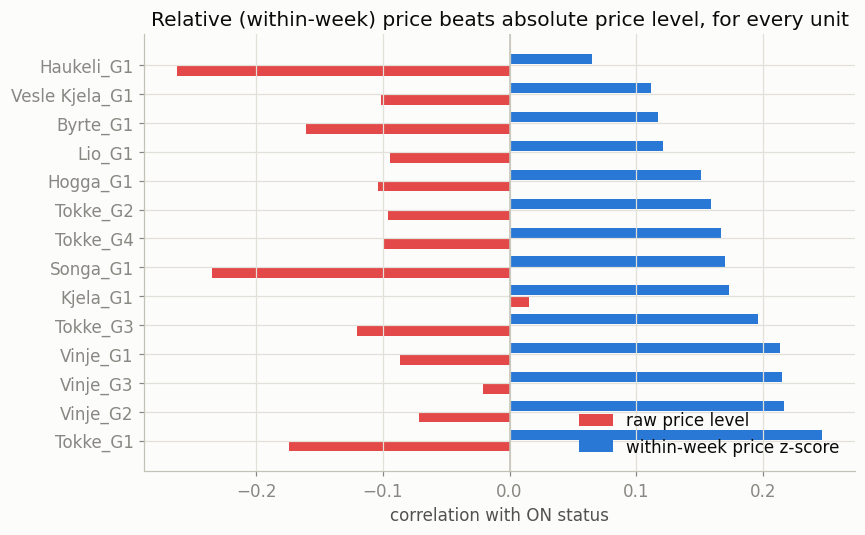
\includegraphics[width=0.75\linewidth]{figures/eda_09_price_corr_raw_vs_within_week_z.png}
  \caption{Per-unit correlation of ON status with raw price vs.\ within-case price z-score.}
  \label{fig:eda-price-corr}
\end{figure}

\finding{For every single unit, correlation with ON status flips from weak/negative
(raw price level) to consistently positive ($\sim$0.15--0.25) when price is normalized
\emph{within each case's own 168-hour window} (Figure~\ref{fig:eda-price-corr}). The optimizer
reacts to ``is this hour relatively good within this week's water/price outlook,'' not to
absolute price. High-price years like 2022 also tend to be scarce-water years, where the
optimizer conserves water and runs fewer units despite high prices --- explaining the
year-level negative relationship in Figure~\ref{fig:eda-yearly}. Implication: within-case
normalized price and a \texttt{price $-$ water\_value} spread are promising engineered features,
likely more robust to the 2022-style regime shift than raw levels.}

\subsubsection*{Extended data.} The topology YAML gives an explicit plant $\to$ upstream-reservoir
map (used above to explain the Tokke/Vinje correlation) and defines the wider reservoir/river/
tunnel graph. The environmental constraint files are sparse and seasonal --- only a handful of
reservoirs/rivers are ever constrained, and only part of the year --- suggesting a binary
``currently constrained'' flag would be a more useful encoding than the raw (mostly-zero)
values, if we decide to use the extended data at all.

\subsection{2026-09-21 --- Centralizing the scattered data into a modeling table}
\label{sec:modeling-table}

\subsubsection*{Motivation.} The raw source files are scattered across several CSVs at different
native granularities (hourly price/inflow, daily storage/water value, one row per 168-hour case
for labels). Keeping them separate is fine, and good practice, as the unmodified source of
truth. But a supervised model needs one row = one example, features..., target at the end ---
so before any modeling, everything is joined once into a flat table, which also forces explicit,
one-time decisions about how sources at different granularities align to a row and where the
train/test boundary falls.

\subsubsection*{Design decisions (discussed and agreed before building).}
\begin{itemize}
  \item \textbf{Row granularity: one row per (case, hour).} Considered alternatives: one row per
    (case, hour, unit) (long format, $\sim$6.9M rows, simplest per-row model but duplicates
    case/hour features 14$\times$ and drops the multi-unit correlation structure from
    Section~\ref{sec:eda}), and one row per case (fully wide, 2{,}922 rows but 2{,}352 target
    columns, awkward for standard tabular models). Case+hour keeps a manageable row count while
    keeping all 14 units' targets on one row, so a model can see them jointly if we want it to.
  \item \textbf{Raw joins only, no engineered features.} No normalization, no lags, no derived
    columns at this stage --- feature engineering (e.g.\ the within-case price normalization
    from Section~\ref{sec:eda}) is treated as a separate, explicit step.
  \item \textbf{Core dataset (\texttt{data/kernel/}) only.} Extended data (topology,
    constraints) intentionally left out until there's a concrete reason to use it.
  \item \textbf{Per-reservoir columns kept separate}, not pre-aggregated (17 inflow + 17 storage
    + 17 water-value columns, individually named), so nothing is thrown away before we've
    decided how to use it.
\end{itemize}

\subsubsection*{Implementation.} \texttt{src/build\_modeling\_table.py}. Daily-native features
(storage, water value) are repeated across each day's 24 hours since they're only observed once
per day. Targets are reshaped from the labels file's wide format
(\texttt{result\_committed\_<unit>\_t<hour>}) into one \texttt{on\_<unit>} column per unit.
Output:

\begin{itemize}
  \item \texttt{data/processed/train\_hourly.parquet} --- 490{,}896 rows (2{,}922 cases
    $\times$ 168 hours) $\times$ 72 columns (5 id/time columns, 53 raw features, 14 targets).
  \item \texttt{data/processed/test\_hourly.parquet} --- 121{,}800 rows (725 cases $\times$
    168 hours) $\times$ 58 columns (same features, no targets).
\end{itemize}

\finding{Spot-checked the join against raw source files (a mid-case UC label, a price value, a
storage value at a specific timestamp) --- all matched exactly. No missing values after joining
any feature column.}

\subsection{2026-09-21 --- Baseline: 14 independent XGBoost models}
\label{sec:baseline}

\subsubsection*{Goal.} Get a first read on how hard the problem is, and where the weaknesses are,
before investing in feature engineering or a more complex architecture. Full notebook:
\texttt{src/modeling/baseline\_xgboost.ipynb}.

\subsubsection*{Design decisions (discussed and agreed before running).}
\begin{itemize}
  \item \textbf{Chronological validation split}, not random: train on 2015--2021, validate on
    held-out \textbf{2022} in full. A random split would let the model see neighboring hours
    from the same case/week, inflating the score; holding out 2022 whole also directly tests
    robustness to the price-crisis regime shift identified in Section~\ref{sec:eda}.
  \item \textbf{One independent XGBoost binary classifier per unit} (14 models total), each
    trained on the same 54 raw features from \texttt{train\_hourly.parquet}
    (\texttt{hour} + \texttt{price\_eur\_mwh} + 18 inflow + 17 storage + 17 water\_value
    columns) --- the simplest architecture that matches the table as built.
  \item \textbf{Metric}: the competition's own \texttt{kaggle\_metric.py} (micro-average
    ROC-AUC), applied for real by reshaping validation predictions back into the competition's
    wide submission format, plus a per-unit AUC breakdown the pooled metric hides.
\end{itemize}

\subsubsection*{Split sizes.} Fit: 2{,}557 cases / 429{,}576 rows (2015--2021). Validation: 365 cases
/ 61{,}320 rows (2022).

\subsubsection*{Results.}

\begin{table}[htbp]
  \centering
  \caption{Per-unit ROC-AUC on the 2022 validation set, baseline model.}
  \label{tab:baseline-auc}
  \begin{tabular}{lr}
    \toprule
    Unit & AUC \\
    \midrule
    Byrte\_G1        & 0.751 \\
    Vesle\_Kjela\_G1 & 0.724 \\
    Lio\_G1          & 0.713 \\
    Songa\_G1        & 0.677 \\
    Hogga\_G1        & 0.655 \\
    Kjela\_G1        & 0.619 \\
    Vinje\_G3        & 0.580 \\
    Tokke\_G1        & 0.577 \\
    Haukeli\_G1      & 0.564 \\
    Tokke\_G2        & 0.557 \\
    Tokke\_G3        & 0.528 \\
    Vinje\_G2        & 0.524 \\
    Vinje\_G1        & 0.519 \\
    Tokke\_G4        & 0.504 \\
    \midrule
    \textbf{Overall (micro-average, official metric)} & \textbf{0.647} \\
    \bottomrule
  \end{tabular}
\end{table}

\begin{figure}[htbp]
  \centering
  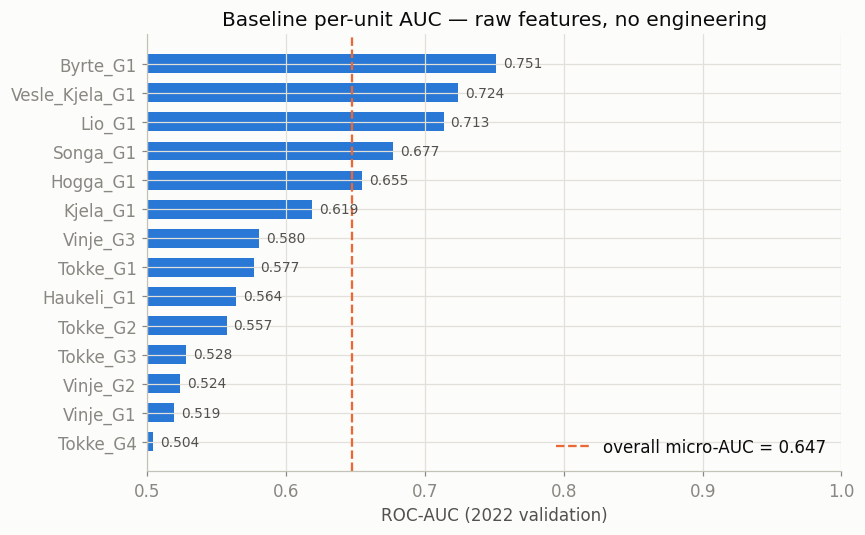
\includegraphics[width=0.75\linewidth]{figures/baseline_01_per_unit_auc.png}
  \caption{Per-unit AUC, baseline model, 2022 validation.}
  \label{fig:baseline-auc}
\end{figure}

\begin{figure}[htbp]
  \centering
  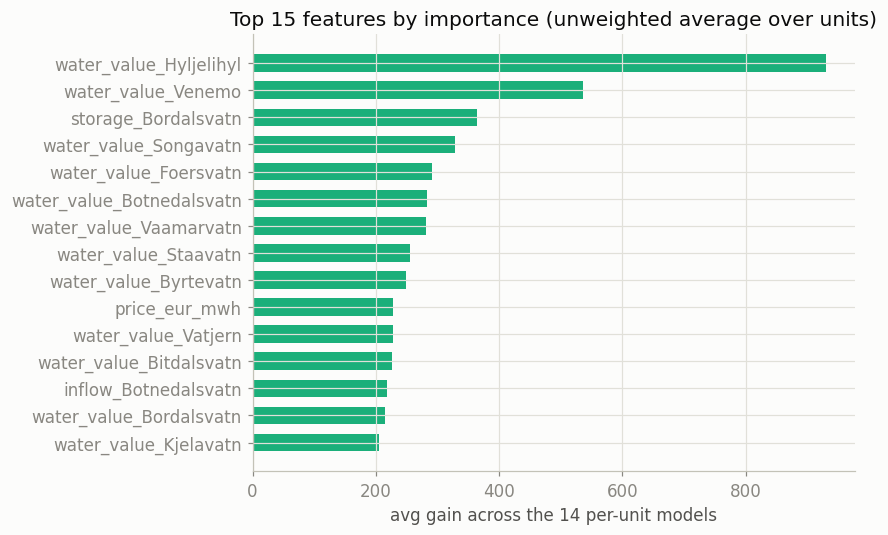
\includegraphics[width=0.75\linewidth]{figures/baseline_02_feature_importance.png}
  \caption{Top 15 features by average gain across the 14 per-unit models.}
  \label{fig:baseline-importance}
\end{figure}

\finding{Overall micro-AUC of 0.647 --- a workable but mediocre first baseline. Per-unit AUC
spans 0.50 (near-random, Tokke\_G4) to 0.75 (Byrte\_G1). The weakest units are almost exactly
the multi-unit Tokke (4 units) and Vinje (3 units) group --- the same units flagged as strongly
cross-correlated in Section~\ref{sec:eda}. Hypothesis (not yet tested): at a multi-unit plant,
\emph{how many} units are on may be easier to predict from price/water data than \emph{which
specific} unit(s), and 14 independent per-unit models have no way to share that information.}

\finding{Feature importance (Figure~\ref{fig:baseline-importance}) is smeared across many
similar reservoir columns rather than concentrated --- consistent with the observation that
every unit's model currently sees all 53 raw features (all 17 reservoirs), not just the ones
plausibly relevant to that unit's plant.}

This result (and every future one, scored the same way) is tracked in
\texttt{report/leaderboard.md} as it's produced, per \texttt{report\_rules.md}.

\subsection{2026-09-21 --- Discussion: graph structure, joint modeling, and next baseline}
\label{sec:discussion-next}

The Tokke/Vinje weak spot in Section~\ref{sec:baseline} prompted a discussion of whether the
watercourse topology (Section~\ref{sec:eda}) should be used more directly, e.g.\ via a graph
neural network over the reservoir/plant graph.

\subsubsection*{GNN considered and set aside for now.} The topology does explain the Tokke/Vinje
correlation physically (Vinje's reservoir cascades into Vinjevatn, which Tokke draws from), so a
graph-based architecture is conceptually reasonable. But: the graph is small ($\sim$22 nodes)
and \emph{identical} at train and test time, so a GNN's main advantage --- generalizing to
unseen graph structure --- doesn't really apply here. It would also be a large implementation
jump (new framework, per-case graph batching, a training loop) relative to what's been built so
far.

\subsubsection*{A premise checked and corrected.} The natural cheaper alternative --- adding each
plant's upstream-reservoir features explicitly --- turned out to already be moot: the current
modeling table (Section~\ref{sec:modeling-table}) already joins \emph{all} 17 reservoirs' data
into every row, so every unit's baseline model already had access to its neighbors' data. The
real gap is therefore not missing input features, but that the 14 units are modeled
\textbf{independently} and can't share information about each other's predictions --- a
correlated-\emph{output} problem, not a missing-\emph{input} problem.

\subsubsection*{Multi-output architectures considered.} To model 14 correlated binary outputs
without exploding the output space (treating the full ON/OFF vector as one
$2^{14}=16{,}384$-way categorical label was explicitly ruled out --- almost all combinations
never occur, and it discards the partial-credit nature of AUC scoring):
\begin{itemize}
  \item \textbf{Multi-output trees}: a single boosted model where each leaf stores a vector of
    14 probabilities instead of one scalar, with splits chosen to jointly improve all 14
    outputs (XGBoost's \texttt{multi\_strategy="multi\_output\_tree"}). Leaf count stays linear
    in tree depth, not exponential in the number of units.
  \item \textbf{Classifier chains}: feed earlier units' predicted probabilities as extra input
    features to later units' models, in some order. Simple to bolt onto the existing per-unit
    XGBoost setup.
  \item Briefly noted: a shared-trunk neural net with 14 sigmoid output heads (bigger jump from
    the current XGBoost-based approach; not pursued yet).
\end{itemize}

\subsubsection*{Decision.} Explicitly \emph{not} anchoring to the earlier plan of testing the
cheapest hypothesis first (Section~\ref{sec:eda}'s within-case price normalization) before
trying anything else --- this is an early stage of a multi-week project, and it's fine to
resequence as better questions surface. Next step agreed: build a \textbf{multi-output tree}
model as the next baseline and compare directly against the 14-independent-model baseline in
Section~\ref{sec:baseline}, using the same validation protocol (train 2015--2021, validate on
2022, score with \texttt{kaggle\_metric.py}).

\subsection{2026-09-21 --- Baseline 2: joint multi-output tree}
\label{sec:multioutput}

\subsubsection*{Goal.} Test directly whether the Tokke/Vinje weakness in the baseline
(Section~\ref{sec:baseline}) is a correlated-\emph{output} problem, as hypothesized in
Section~\ref{sec:discussion-next}. Full notebook:
\texttt{src/modeling/multioutput\_tree.ipynb}.

\subsubsection*{Design.} Everything held identical to baseline 1 --- same 54 raw features, same
hyperparameters (\texttt{n\_estimators=200}, \texttt{max\_depth=6}, \texttt{learning\_rate=0.1},
subsample/colsample 0.8), same chronological split (train 2015--2021, validate on held-out
2022), same \texttt{kaggle\_metric.py} scoring --- with exactly one change: a single
\texttt{XGBClassifier} with \texttt{multi\_strategy="multi\_output\_tree"}, trained on all 14
targets jointly, instead of 14 independent single-output models. Each leaf of each tree stores a
vector of 14 probabilities; split choices are optimized jointly across units. This isolates the
independent-vs-joint modeling question specifically, with no other confound.

\subsubsection*{Results.}

\begin{table}[htbp]
  \centering
  \caption{Baseline 1 (independent) vs.\ baseline 2 (joint multi-output tree), 2022 validation.}
  \label{tab:multioutput-auc}
  \resizebox{\linewidth}{!}{%
  \begin{tabular}{lrrr}
    \toprule
    Unit & Baseline 1 (independent models) & Baseline 2 (joint multi-output tree) & $\Delta$ \\
    \midrule
    Tokke\_G3        & 0.528 & 0.656 & +0.129 \\
    Tokke\_G4        & 0.504 & 0.616 & +0.112 \\
    Tokke\_G1        & 0.577 & 0.687 & +0.111 \\
    Vinje\_G1        & 0.519 & 0.622 & +0.102 \\
    Hogga\_G1        & 0.655 & 0.745 & +0.090 \\
    Vinje\_G2        & 0.524 & 0.609 & +0.085 \\
    Vesle\_Kjela\_G1 & 0.724 & 0.773 & +0.049 \\
    Tokke\_G2        & 0.557 & 0.598 & +0.041 \\
    Vinje\_G3        & 0.580 & 0.615 & +0.035 \\
    Byrte\_G1        & 0.751 & 0.784 & +0.033 \\
    Kjela\_G1        & 0.619 & 0.636 & +0.017 \\
    Haukeli\_G1      & 0.564 & 0.554 & $-$0.010 \\
    Lio\_G1          & 0.713 & 0.656 & $-$0.057 \\
    Songa\_G1        & 0.677 & 0.597 & $-$0.080 \\
    \midrule
    \textbf{Overall (micro-average, official metric)} & \textbf{0.647} & \textbf{0.687} & \textbf{+0.040} \\
    \bottomrule
  \end{tabular}%
  }
\end{table}

\begin{figure}[htbp]
  \centering
  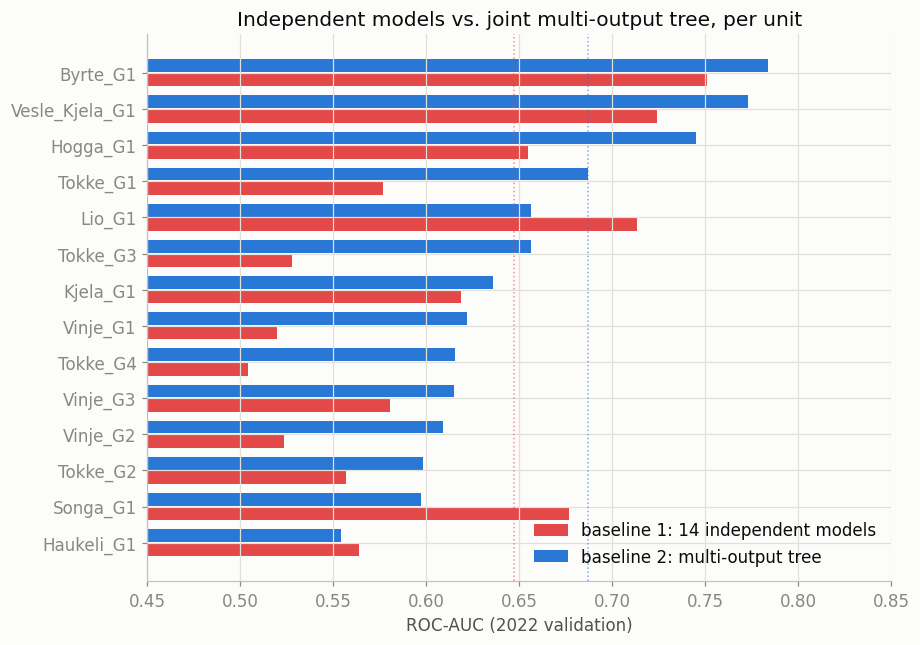
\includegraphics[width=0.85\linewidth]{figures/multioutput_01_per_unit_comparison.png}
  \caption{Per-unit AUC, baseline 1 vs.\ baseline 2, 2022 validation.}
  \label{fig:multioutput-comparison}
\end{figure}

\begin{figure}[htbp]
  \centering
  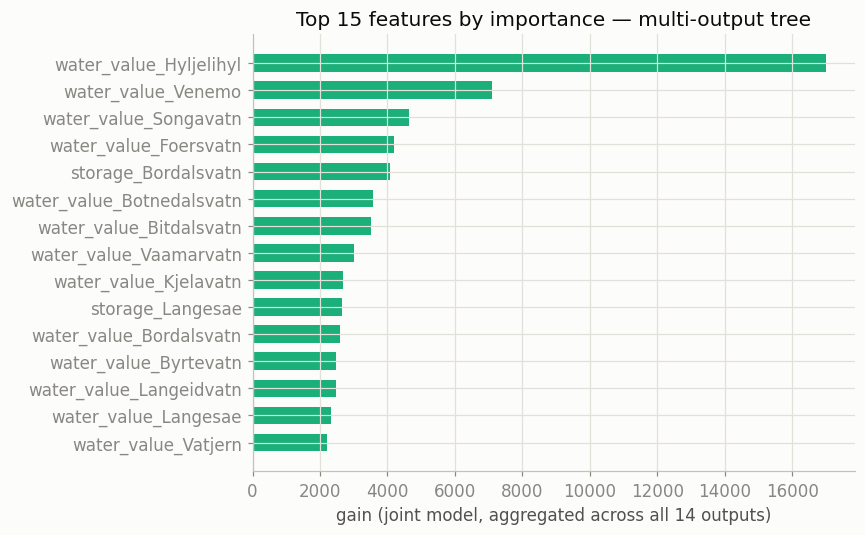
\includegraphics[width=0.75\linewidth]{figures/multioutput_02_feature_importance.png}
  \caption{Top 15 features by gain, joint multi-output model.}
  \label{fig:multioutput-importance}
\end{figure}

\finding{Overall micro-AUC improves from 0.647 to \textbf{0.687} ($+0.040$), and confirms the
hypothesis from Section~\ref{sec:baseline}: the units that improve \emph{most} are almost
exactly the previously-weakest multi-unit-plant units --- all four Tokke units and all three
Vinje units gain $+0.03$ to $+0.13$ AUC, with Hogga\_G1 (topologically adjacent to both, per
Section~\ref{sec:eda}) also improving substantially. Modeling the units jointly does let the
tree exploit the cross-unit correlation that 14 independent models couldn't see.}

\finding{Not a uniform win: \textbf{Songa\_G1 and Lio\_G1 got worse} ($-0.080$ and $-0.057$),
and these were the two best-performing units in baseline 1. Working hypothesis, not yet tested:
the joint model has the same total tree budget (200 trees) shared across all 14 outputs, i.e.\
roughly $14\times$ less dedicated capacity per unit than baseline 1's 200-trees-\emph{each}
setup --- units that didn't need cross-unit information to begin with may simply have lost
modeling capacity to units that did. Worth revisiting (e.g.\ more estimators for the joint
model) before treating this architecture as strictly better.}
\supersededby{sec:capacity}{this capacity hypothesis is tested directly, with a nuanced partial
confirmation.}

This result is tracked in \texttt{report/leaderboard.md} alongside baseline 1.

\subsection{2026-09-21 --- Does more capacity fix the multi-output model's regressed units?}
\label{sec:capacity}

\subsubsection*{Goal.} Section~\ref{sec:multioutput} flagged, but did not test, the hypothesis
that Songa\_G1 and Lio\_G1 regressed under the joint multi-output model because 200 trees
shared across 14 outputs gives far less dedicated capacity per unit than baseline 1's
200-trees-\emph{each}. Full notebook: \texttt{src/modeling/multioutput\_tree\_capacity.ipynb}.

\subsubsection*{Method.} Trained once to 3{,}000 trees (no early stopping; see below for why),
identical features/hyperparameters to Section~\ref{sec:multioutput} otherwise. Checked the
official \texttt{kaggle\_metric.py} micro-AUC at $\sim$45 checkpoints via
\texttt{predict\_proba(..., iteration\_range=(0,k))}, which reuses the one trained model rather
than retraining at every candidate tree count.

\finding{XGBoost's own multi-output \texttt{eval\_metric="auc"} does \emph{not} match the
official micro-AUC --- it tracks consistently lower and noisier (Figure~\ref{fig:capacity-internal}).
Almost certainly a macro-average across the 14 outputs rather than a pooled/micro calculation.
Using it for early stopping in this multi-output setup would optimize the wrong target, which is
why this run used a fixed generous cap and our own checkpointing instead.}

\begin{figure}[htbp]
  \centering
  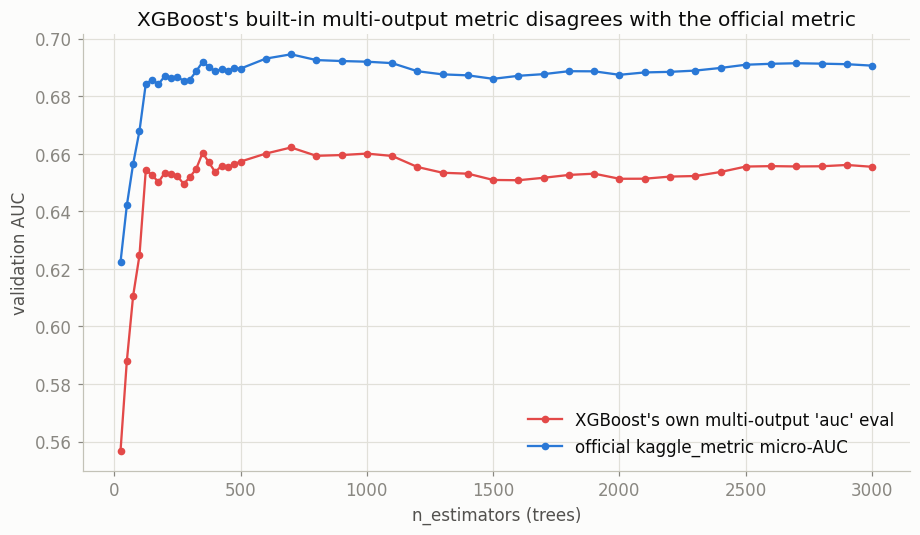
\includegraphics[width=0.8\linewidth]{figures/capacity_01_internal_vs_official.png}
  \caption{XGBoost's internal multi-output AUC vs.\ the official micro-AUC.}
  \label{fig:capacity-internal}
\end{figure}

\subsubsection*{Results: a real plateau, then a real decline.}

\begin{figure}[htbp]
  \centering
  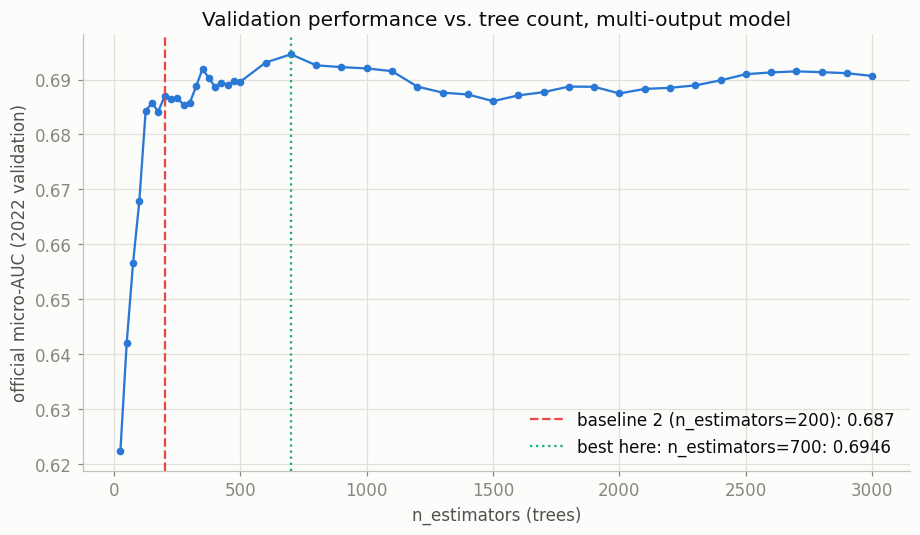
\includegraphics[width=0.8\linewidth]{figures/capacity_02_plateau_curve.png}
  \caption{Official micro-AUC vs.\ tree count, up to 3{,}000 trees.}
  \label{fig:capacity-plateau}
\end{figure}

\finding{Validation performance rises sharply to $\sim$150 trees, keeps climbing gently to a
peak at \textbf{$n_{\text{estimators}}=700$ (micro-AUC 0.6946)}, then genuinely declines to
$\sim$0.686 by 1{,}500 trees --- a real $\sim$0.008 drop, not noise --- before a mild, incomplete
recovery out to 3{,}000 that never regains the 700-tree peak (Figure~\ref{fig:capacity-plateau}).
$n_{\text{estimators}}=700$ is a $+0.0076$ improvement over baseline 2's original
$n_{\text{estimators}}=200$ (0.687 $\to$ 0.6946), confirming the model was undertrained, not
just differently structured.}

\begin{figure}[htbp]
  \centering
  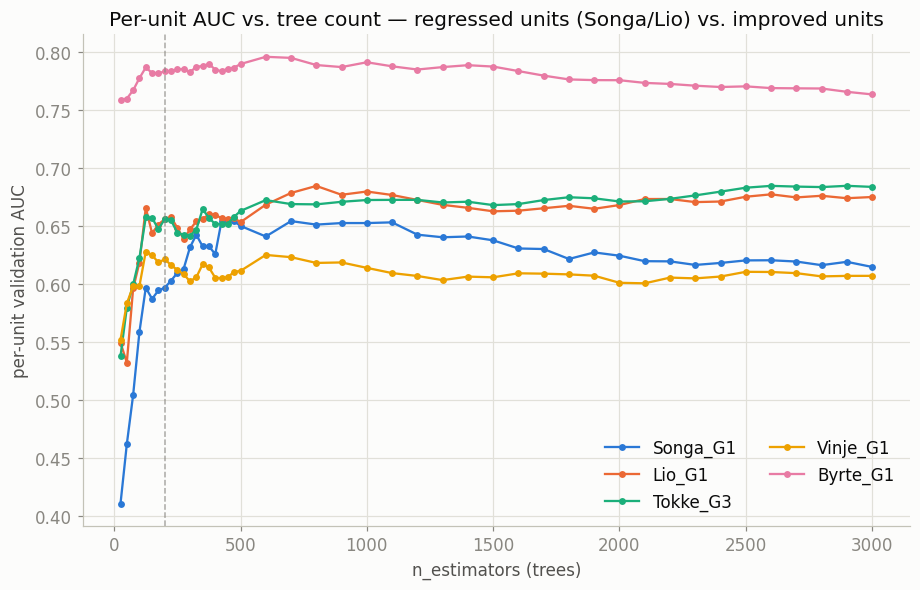
\includegraphics[width=0.8\linewidth]{figures/capacity_03_per_unit_curves.png}
  \caption{Per-unit AUC vs.\ tree count: regressed units (Songa\_G1, Lio\_G1) vs.\ improved/strong units.}
  \label{fig:capacity-per-unit}
\end{figure}

\finding{\textbf{The capacity hypothesis is only partially right.} At $n_{\text{estimators}}=700$,
Songa\_G1 recovers from 0.597 (at 200 trees) to 0.655, and Lio\_G1 from 0.656 to 0.679
(Figure~\ref{fig:capacity-per-unit}) --- real improvement. But neither returns to its baseline-1
independent-model score (Songa\_G1: 0.677, Lio\_G1: 0.713) anywhere in the swept range; both
plateau and then decline alongside the overall curve rather than continuing to close the gap.
So: more capacity was genuinely part of the story, but something else about joint modeling still
costs these two specific units relative to modeling them independently. Left as an open question
for the next round of exploratory analysis rather than chased further here.}

\subsubsection*{Decision: adopt $n_{\text{estimators}}=300$, not the argmax.}
The sweep's argmax is 700, but the whole region from $\sim$125 to $\sim$500 trees is a noisy
plateau spanning only $\sim$0.006 AUC, measured on a \emph{single} validation year. Selecting the
argmax of a noisy validation curve is itself a form of overfitting --- to the validation set
rather than the training set --- and 700 would likely not be the argmax on a different holdout
year. We therefore adopt \textbf{$n_{\text{estimators}}=300$} as the standing default: inside the
stable plateau, cheaper to train, and not tuned to a single noisy peak. Measured score at 300 is
0.6858, nominally $0.0012$ below the $n=200$ run --- a difference well inside the noise of this
plateau, and not treated as meaningful. Revisit once there is a more robust validation scheme
(multiple holdout years or proper time-series CV) that could distinguish these points.

Updated in \texttt{report/leaderboard.md} as \texttt{xgb\_multioutput\_tree\_n700}.

\subsection{2026-09-21 --- EDA round 2: what actually makes this problem hard}
\label{sec:eda-round-2}

Round 1 (Section~\ref{sec:eda}) characterised the data. This round targets the structure of the
prediction problem itself, to motivate features and architecture. Full notebook:
\texttt{src/EDA/eda\_round2.ipynb}. Twelve findings; the first four change how we should think
about the task.

\subsubsection*{The labels are not self-consistent.}
Cases are daily rolling, so consecutive cases overlap on 144 identical wall-clock hours (case
$N$'s hour $24{+}h$ is the same real timestamp as case $N{+}1$'s hour $h$), solved by SHOP from
essentially the same physical state.

\begin{figure}[htbp]
  \centering
  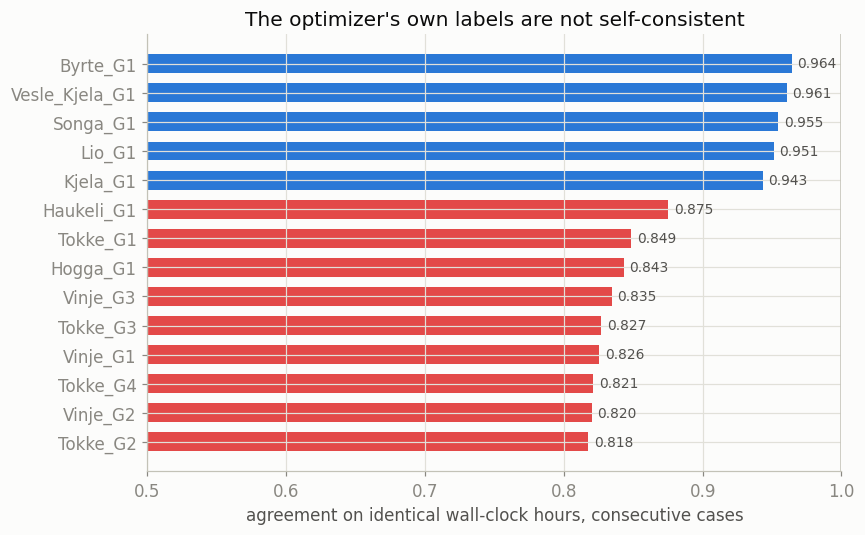
\includegraphics[width=0.72\linewidth]{figures/eda2_01_label_self_agreement.png}
  \caption{Agreement between consecutive cases on identical wall-clock hours.}
  \label{fig:eda2-agreement}
\end{figure}

\finding{\textbf{(1)} The same physical hour, re-solved one day later under a different 168-hour
horizon, gets a \emph{different} commitment decision \textbf{12\% of the time overall, and
$\sim$18\% for the Tokke and Vinje units} (Figure~\ref{fig:eda2-agreement}). This is not
measurement noise --- it is the optimizer reacting to end-of-horizon boundary conditions that a
wall-clock-indexed model cannot observe. It is an effective ceiling on achievable accuracy.}
\supersededby{sec:eda-round-3}{the ``effective ceiling'' inference is withdrawn --- the 12\% measurement stands, but it does not bound AUC.}

\begin{figure}[htbp]
  \centering
  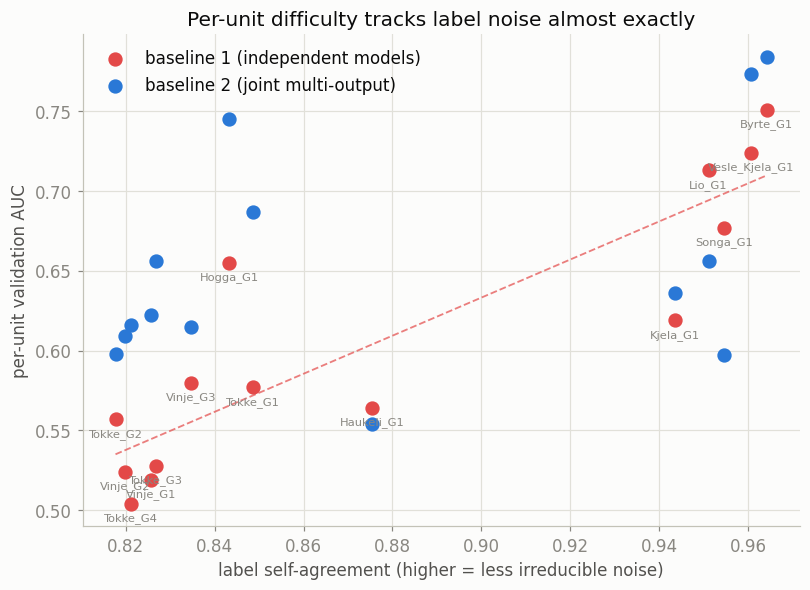
\includegraphics[width=0.72\linewidth]{figures/eda2_02_noise_vs_auc.png}
  \caption{Per-unit label self-agreement vs.\ per-unit validation AUC, both baselines.}
  \label{fig:eda2-noise-auc}
\end{figure}

\finding{\textbf{(2)} Label self-agreement correlates \textbf{$r=0.88$} with baseline-1 per-unit
AUC --- about \textbf{78\% of the variance in per-unit difficulty is explained by label noise
alone}, not by our features (Figure~\ref{fig:eda2-noise-auc}). The correlation drops to $0.42$
for the joint multi-output model, which is precisely the mechanism behind
Section~\ref{sec:multioutput}: pooling let the noisy Tokke/Vinje units borrow signal from their
correlated neighbours. It also finally explains the Songa\_G1 / Lio\_G1 regression left open in
Section~\ref{sec:capacity} --- those are the \emph{cleanest} units (95--96\% self-agreement),
and joint modelling pooled them with seven much noisier ones.}

\subsubsection*{The units inside a plant are identical, and strictly merit-ordered.}

\begin{figure}[htbp]
  \centering
  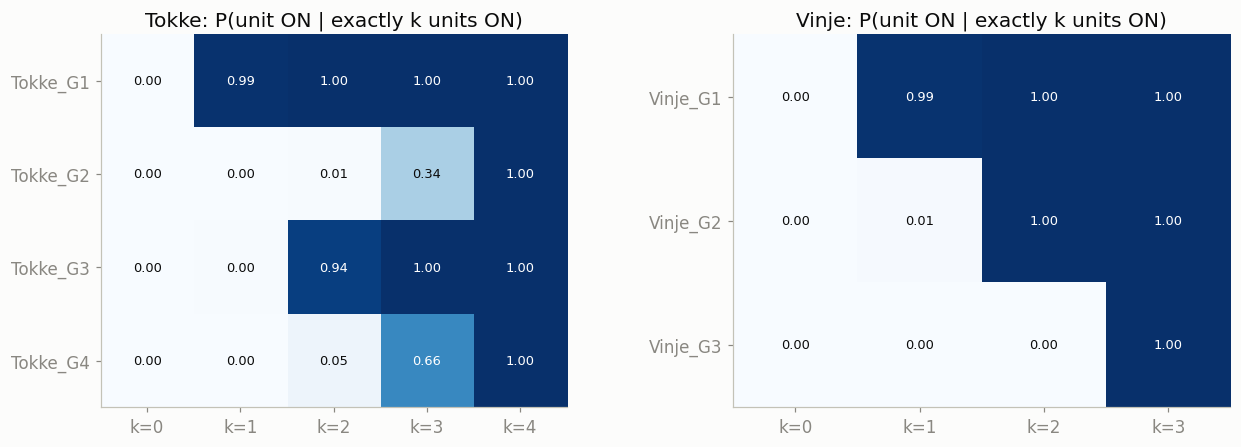
\includegraphics[width=0.95\linewidth]{figures/eda2_03_merit_order.png}
  \caption{$P(\text{unit ON} \mid \text{exactly } k \text{ units ON at the plant})$.}
  \label{fig:eda2-merit}
\end{figure}

\finding{\textbf{(3)} Every generator within a plant is \emph{physically identical} (Tokke:
4$\times$ $p_{\max}=107.5$\,MW; Vinje: 3$\times$ $p_{\max}=100$\,MW --- from the topology YAML we
had not been using). Commitment follows a near-strict merit order
(Figure~\ref{fig:eda2-merit}): Vinje is G1 $\to$ G1+G2 $\to$ all; Tokke is G1 $\to$ G1+G3 $\to$
then G4 or G2. \textbf{Knowing only how many units are on at a plant predicts exactly which ones
with 97.8\% (Tokke) and 99.9\% (Vinje) accuracy.}}

\finding{\textbf{(4)} Because the machines are interchangeable, \emph{which} identical unit takes
the marginal slot is partly an arbitrary solver tie-break --- this is the mechanism behind
finding (1). The only genuinely ambiguous slot is Tokke's third (G2 vs.\ G4, 34/66).}
\supersededby{sec:feature-themes}{penstock sharing explains the G1$\to$G3 ordering --- part of what looked arbitrary is hydraulic structure.}

\medskip
\noindent\textbf{Design implication.} The 14-output problem is really a small number of
\emph{per-plant count} problems plus a near-deterministic lookup. Predicting counts --- ordinal,
and far less noisy --- then expanding via merit order is a better-posed target than 14
individually-noisy binaries. This is the strongest architectural lead we have.

\subsubsection*{Remaining findings.}

\begin{figure}[htbp]
  \centering
  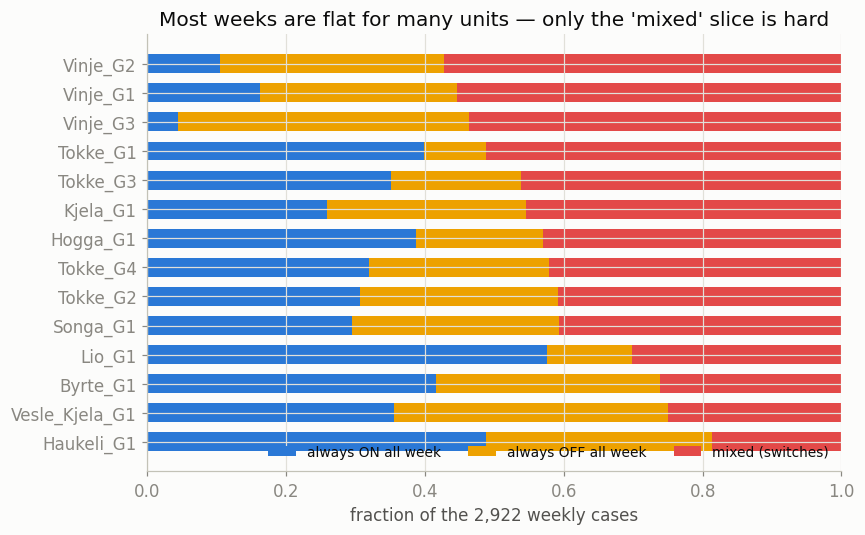
\includegraphics[width=0.72\linewidth]{figures/eda2_04_flat_vs_mixed.png}
  \caption{Share of weekly cases that are flat (never switch) vs.\ mixed, per unit.}
  \label{fig:eda2-flat}
\end{figure}

\finding{\textbf{(5)} Many weeks are completely flat: Haukeli\_G1 never switches in \textbf{81\%}
of weeks, Vesle\_Kjela\_G1 in 75\%, Byrte\_G1 in 74\% (Figure~\ref{fig:eda2-flat}). Only the
``mixed'' slice is genuinely hard, which suggests splitting ``does this unit move at all this
week?'' from ``when does it move?''.}

\begin{figure}[htbp]
  \centering
  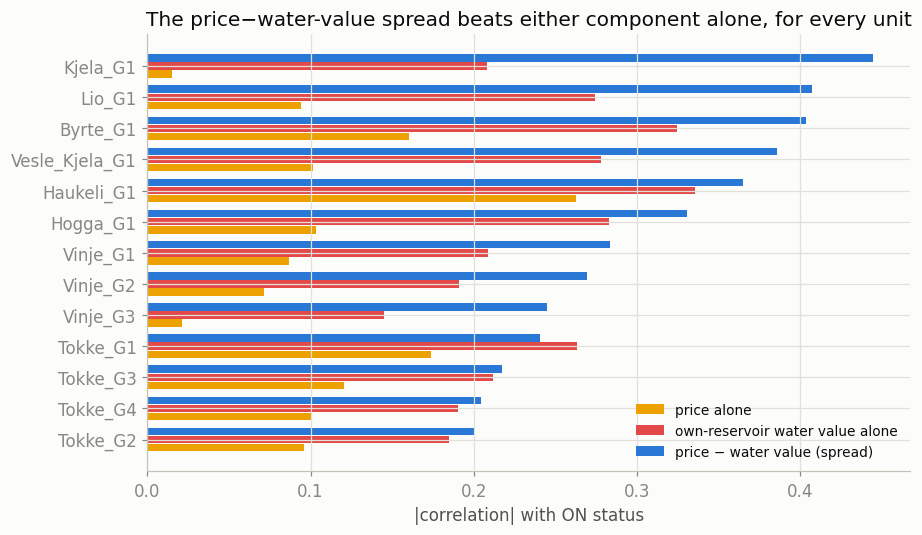
\includegraphics[width=0.78\linewidth]{figures/eda2_05_spread_vs_components.png}
  \caption{$|$correlation$|$ with ON status: price, own-reservoir water value, and their spread.}
  \label{fig:eda2-spread}
\end{figure}

\finding{\textbf{(6)} \texttt{storage\_Vatjern} and \texttt{storage\_Hyljelihyl} are
\textbf{literally constant} --- zero information. (The dataset PDF notes both reservoirs lack
historical records and were assumed 50\% full.) Drop them.}

\finding{\textbf{(7)} The \textbf{price $-$ own-reservoir water value spread} correlates more
strongly with ON status than either component alone, \emph{for every mapped unit}
(Figure~\ref{fig:eda2-spread}) --- the classic hydropower ``sell now vs.\ store it'' signal, and
the clearest single feature-engineering win available. Not currently in the feature set.}

\finding{\textbf{(8, a correction).} Normalising storage by each reservoir's \texttt{max\_vol} ---
proposed earlier in discussion as an important miss --- is a \textbf{no-op for tree models}: it is
a monotonic per-feature rescale, and trees are invariant to those. The 2462$\times$ spread in
reservoir size only matters for features that \emph{combine} reservoirs (e.g.\ system-wide
percent-full), or for linear/neural models. Recorded so we don't ``fix'' a non-problem.}

\begin{figure}[htbp]
  \centering
  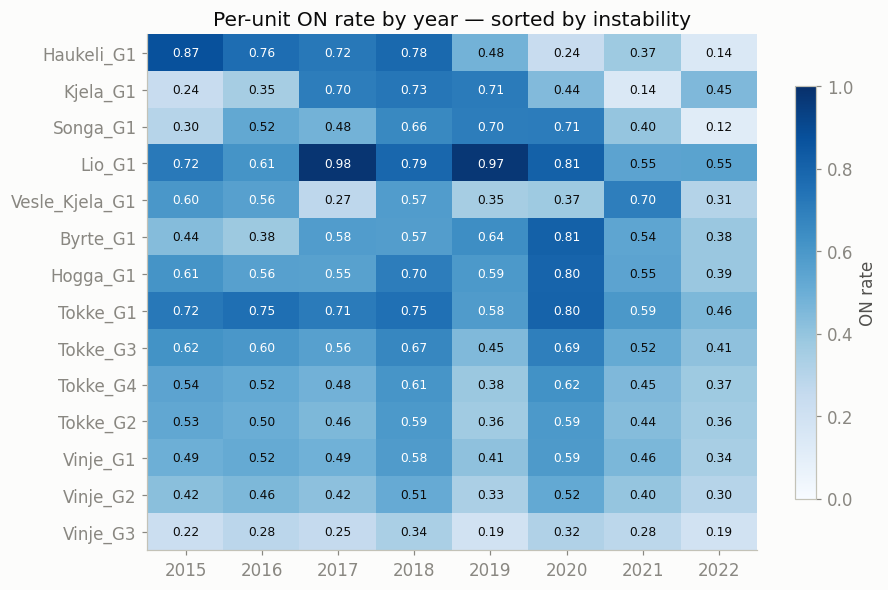
\includegraphics[width=0.78\linewidth]{figures/eda2_06_yearly_instability.png}
  \caption{Per-unit ON rate by year, sorted by instability.}
  \label{fig:eda2-yearly}
\end{figure}

\finding{\textbf{(9)} Severe per-unit non-stationarity: \textbf{Haukeli\_G1 collapses from 0.87
(2015) to 0.14 (2022)}; Songa\_G1 swings $0.30 \to 0.71 \to 0.12$
(Figure~\ref{fig:eda2-yearly}). These are structural changes in plant operation, not noise, and a
\emph{stronger} effect than the 2022 price spike flagged in Section~\ref{sec:eda}. Argues for
recency weighting or a shorter, more recent training window.}

\finding{\textbf{(10)} \texttt{min\_volume} constraints bind for exactly three reservoirs and only
in \textbf{July--October} --- a clean seasonal regime flag.}

\finding{\textbf{(11, a second correction).} \texttt{min\_flow} is \emph{always} active ($>0$ in
100\% of hours) for five of six rivers, so the binary ``is constrained'' flag suggested earlier
would be another constant column. The usable signal is the constraint's \textbf{level} and its
changes, not its existence.}

\finding{\textbf{(12)} The unit $\to$ reservoir map needs \textbf{multi-hop traversal}: Songa has
no direct reservoir edge at all, drawing from Songavatn and Bitdalsvatn through two tunnels and
discharging into Totak. Topology-derived features must walk the graph, not read single-hop edges.}

\subsection{2026-09-21 --- EDA round 3: how should the data be transformed?}
\label{sec:eda-round-3}

Rounds 1--2 asked what is in the data and what makes the problem hard. This round asks the
engineering question: \emph{given tree models, which transformations actually create signal?}
Full notebook: \texttt{src/EDA/eda\_round3.ipynb}.

\subsubsection*{A framing constraint that prunes the search space.}
Trees are invariant to monotonic transforms of a \emph{single} column --- rescaling, logging or
min-max normalising one feature does nothing at all to an XGBoost model. Only transforms that
\emph{combine} information can help, and there are exactly four such families: column
combinations (differences, ratios), time-window aggregates, graph/space aggregates, and
cross-sectional ranks. All feature work should come from those four.

\subsubsection*{Correcting the ``noise ceiling'' claim from round 2.}
Section~\ref{sec:eda-round-2} measured that labels are 12\% self-inconsistent and inferred an
``effective ceiling on achievable accuracy''. The measurement stands; \textbf{the inference was
wrong}, in two specific ways. First, it conflated a label-flip rate with an AUC ceiling --- AUC
is a \emph{ranking} metric, and a model can rank well-ordered probabilities highly even where it
would be wrong at a 0.5 threshold. Second, it assumed the horizon boundary condition was
unobservable; it is not, and is quantified below. External evidence that scores around 0.99 are
attainable on this dataset is consistent with the disagreement being \emph{signal we are not
capturing} rather than noise.

\subsubsection*{Normalisation: which component creates the signal?}

\begin{figure}[htbp]
  \centering
  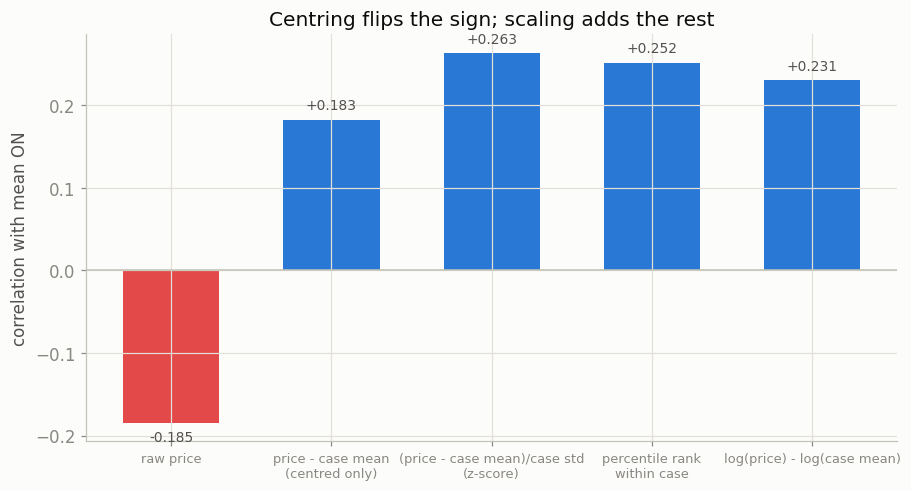
\includegraphics[width=0.78\linewidth]{figures/eda3_01_normalisation_components.png}
  \caption{Correlation with mean ON for five price transformations.}
  \label{fig:eda3-norm}
\end{figure}

\finding{\textbf{(1)} Raw price correlates $-0.185$ with commitment; subtracting the case mean
flips it to $+0.183$; dividing by the case's own standard deviation reaches $+0.263$
(Figure~\ref{fig:eda3-norm}). The two operations do different jobs: \textbf{centring removes the
cross-period scarcity confound} (high-price years are scarce-water years) and \textbf{scaling
makes a $\pm5$ EUR deviation in 2015 comparable to a $\pm100$ EUR deviation in 2022}. Percentile
rank within the case ($+0.252$) captures nearly all of it distribution-free. \emph{Price features
should be case-relative and scale-free, never raw levels.}}

\finding{\textbf{(2)} The opposite rule holds for the price\,$-$\,water-value spread: raw
$+0.241$ vs.\ z-scored within case $+0.114$. The spread is \emph{already} relative --- price
measured against its own opportunity cost --- so normalising twice destroys the cross-case level
information. \textbf{Normalise price; do not normalise the spread.}}

\subsubsection*{The optimizer is forward-looking.}

\begin{figure}[htbp]
  \centering
  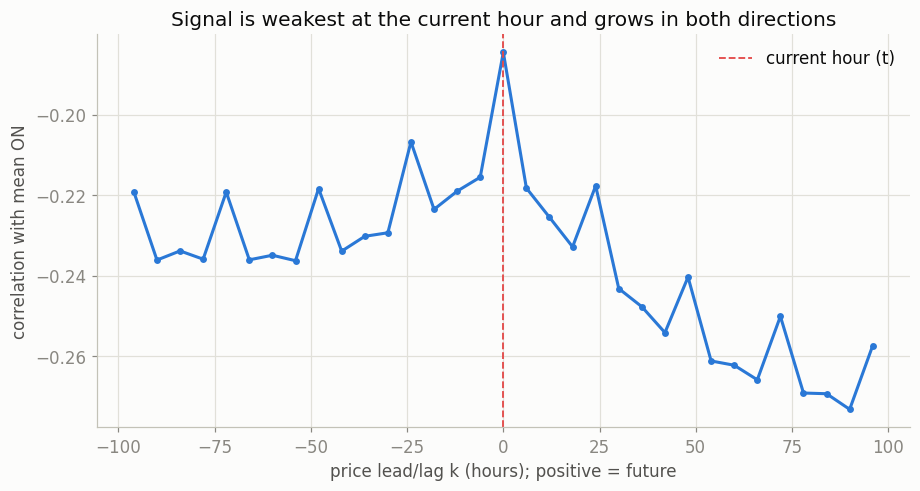
\includegraphics[width=0.78\linewidth]{figures/eda3_02_price_lead_lag.png}
  \caption{Correlation between mean ON and price at lead/lag $k$.}
  \label{fig:eda3-leadlag}
\end{figure}

\finding{\textbf{(3)} The price/commitment correlation is \textbf{weakest at the current hour}
($-0.185$ at $k=0$) and strengthens in \emph{both} directions, peaking around $k=+90$h
($-0.273$) --- see Figure~\ref{fig:eda3-leadlag}. The optimizer uses the whole horizon, and the
\emph{sustained level} of price over multi-day windows matters more than the instantaneous value.
Forward-looking window features are legitimate here because the full 168h price path is known at
solve time.}
\supersededby{sec:eda-round-3b}{this curve ignored case boundaries; the corrected peak is $\approx-0.245$, and the ``legitimacy'' claim is refined there.}

\subsubsection*{Dimensionality and graph structure.}

\begin{figure}[htbp]
  \centering
  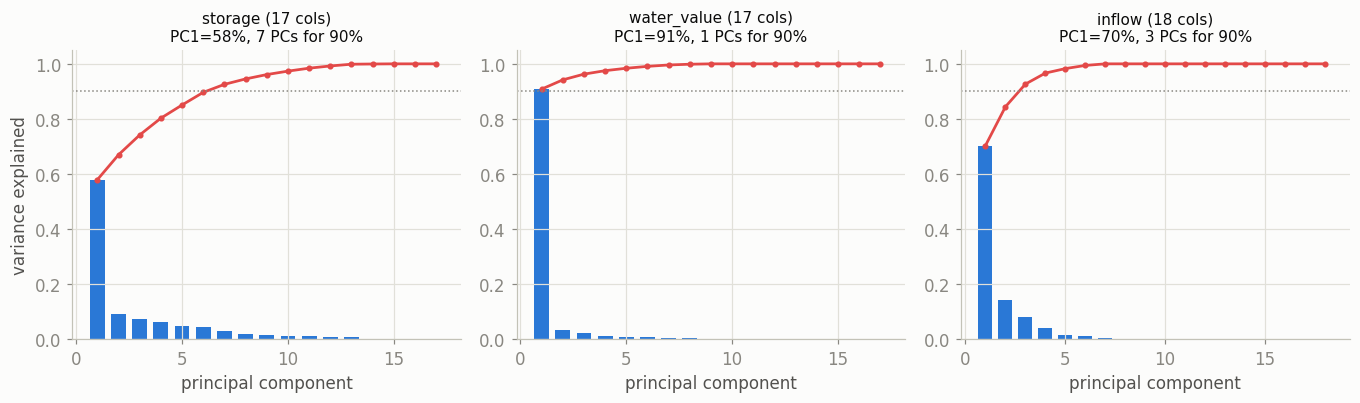
\includegraphics[width=0.95\linewidth]{figures/eda3_03_pca_dimensionality.png}
  \caption{Variance explained by principal components within each feature family.}
  \label{fig:eda3-pca}
\end{figure}

\finding{\textbf{(4)} The 17 water-value columns have \textbf{PC1 $=$ 91\%} of variance --- they
are effectively \emph{one} system-wide scarcity factor (Figure~\ref{fig:eda3-pca}). Inflow needs
3 components for 90\%, storage 7. Adding more per-reservoir water-value columns is near-useless;
the informative decomposition is \textbf{(system common factor) $+$ (reservoir-specific
deviation)}.}

\begin{figure}[htbp]
  \centering
  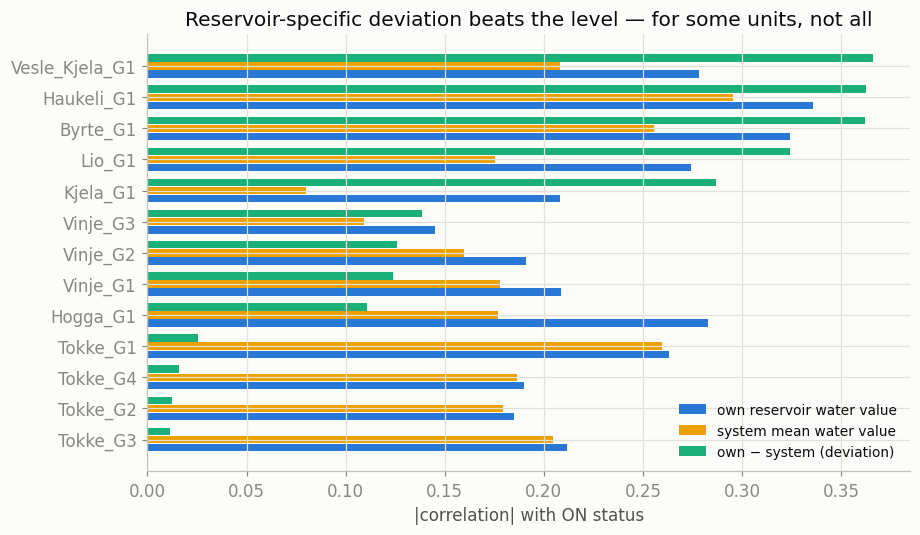
\includegraphics[width=0.78\linewidth]{figures/eda3_04_graph_aggregation.png}
  \caption{Own-reservoir vs.\ system-mean vs.\ own-minus-system water value, per unit.}
  \label{fig:eda3-graph}
\end{figure}

\finding{\textbf{(5)} The \textbf{own $-$ system} water-value deviation is the strongest of the
three for Vesle\_Kjela\_G1 (0.366 vs.\ 0.278), Byrte\_G1, Haukeli\_G1, Kjela\_G1 and Lio\_G1, but
is $\sim$0.01 for the Tokke units because Vinjevatn tracks the system almost perfectly
(Figure~\ref{fig:eda3-graph}). Graph/neighbourhood features help \emph{selectively and per unit}
--- which a single global feature set cannot express.}

\subsubsection*{The unused boundary condition.}

\begin{figure}[htbp]
  \centering
  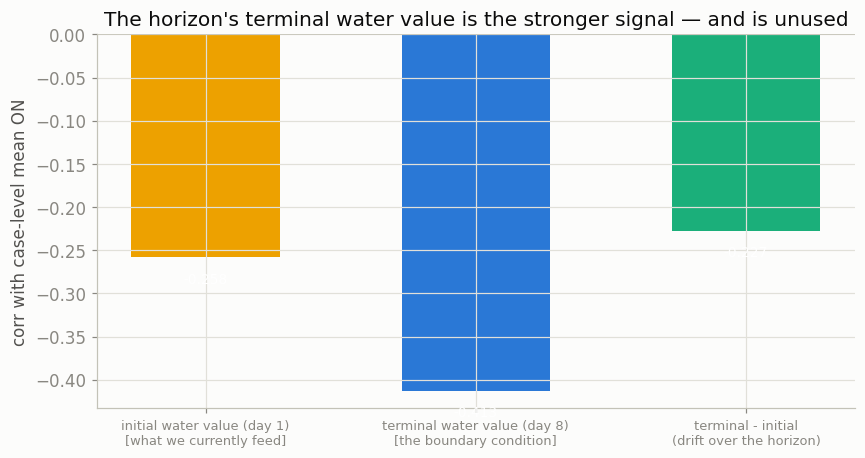
\includegraphics[width=0.72\linewidth]{figures/eda3_05_terminal_water_value.png}
  \caption{Initial vs.\ terminal horizon water value against case-level commitment.}
  \label{fig:eda3-terminal}
\end{figure}

\finding{\textbf{(6)} The dataset documentation states a case's \emph{final} water value is the
value at start $+$ 8 days. We feed the model the \textbf{initial} value and never the terminal
one. The terminal value correlates $\mathbf{-0.41}$ with case-level commitment versus $-0.26$ for
the initial value, and the two differ in \textbf{93\%} of case/reservoir pairs
(Figure~\ref{fig:eda3-terminal}). A genuine per-case boundary condition, documented in the data
and entirely unused.}

\subsubsection*{Two hypotheses tested and refuted.}

\begin{figure}[htbp]
  \centering
  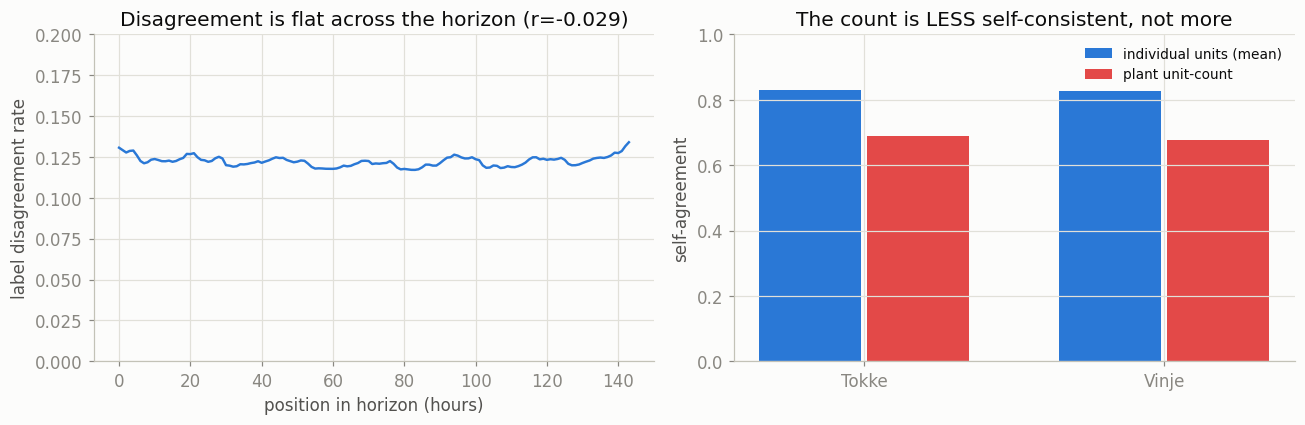
\includegraphics[width=0.95\linewidth]{figures/eda3_06_refuted_hypotheses.png}
  \caption{Left: disagreement vs.\ horizon position. Right: unit vs.\ count self-agreement.}
  \label{fig:eda3-refuted}
\end{figure}

\finding{\textbf{(7, refuted)} I expected label disagreement to concentrate at the end of the
horizon where the boundary condition bites. It is \textbf{flat} ($r = -0.03$). The terminal water
value shapes the whole week's schedule, not just its tail. \emph{No horizon-position sample
weighting is justified.}}

\finding{\textbf{(8, refuted)} I predicted per-plant \emph{counts} would be less noisy than
individual units. They are \textbf{more} noisy (Tokke 0.688 vs.\ 0.829) --- obvious in hindsight,
since a sum disagrees whenever any term does. This does not invalidate the count-based
architecture from Section~\ref{sec:eda-round-2}, but its justification is the merit-order
determinism, \emph{not} a noise reduction. Claim corrected.}

\subsubsection*{Transformation rules established.}
\begin{itemize}
  \item Price features: case-relative and scale-free (z-score or percentile), never raw levels.
  \item The price\,$-$\,water-value spread: use raw, do \emph{not} normalise.
  \item Use multi-day forward \emph{and} backward price windows, not the current hour.
  \item Water value: one common factor plus deviations, not 17 correlated columns.
  \item \texttt{own $-$ system} deviations help selectively, per unit.
  \item Feed the terminal (day-8) water value alongside the initial one.
  \item No horizon-position weighting; counts are not a noise reduction.
\end{itemize}

\subsection{2026-09-21 --- EDA round 3b: point-in-time correctness and temporal transforms}
\label{sec:eda-round-3b}

Round 3a (Section~\ref{sec:eda-round-3}) under-covered the time-series side --- it tested three
hypotheses and refuted two, rather than surveying transformations --- and it contained a
point-in-time error. This entry fixes both. Notebook:
\texttt{src/EDA/eda\_round3b\_temporal.ipynb}.

\subsubsection*{What the documentation actually specifies about test-time availability.}
The task PDF lists input \emph{categories} and states that predictions go to Kaggle. It says
\textbf{nothing} about temporal availability rules. Earlier claims in this log about what is
``available at test time'' were therefore inference, not documented fact. The question is
answerable empirically, so it was checked.

\finding{\textbf{(0, verified)} Every \emph{feature} file extends past the last hour we must
predict (2024-12-31 23:00): price to 2025-12-31, inflow to 2025-10-15, volume and water value to
2025-01-01, both constraint files to 2025-12-31. So all feature sources are genuinely available
for all 725 test cases. \textbf{Labels stop at 2022-12-31}, so any feature derived from past
\emph{targets} --- trailing ON-rate, previous case's decisions --- is unusable beyond the first
test case. The terminal (day$+$8) water value is available for \textbf{724 of 725} cases; only the
final case (2024-12-25) reaches past the file's end and needs a documented fallback.}

\medskip\noindent
A distinction the earlier draft got wrong: \emph{beyond-horizon} future prices (e.g.\ hour 200
when the case ends at 167) are \textbf{permitted} --- nothing forbids them and on a fixed test set
they are not cheating. The only argument against them is that the label-generating optimizer
never saw past its own horizon, so such features describe information the target does not depend
on. That is a modelling judgement to test, not a correctness rule; round 3a overstated it as the
latter.

\subsubsection*{Corrected lead/lag.}

\begin{figure}[htbp]
  \centering
  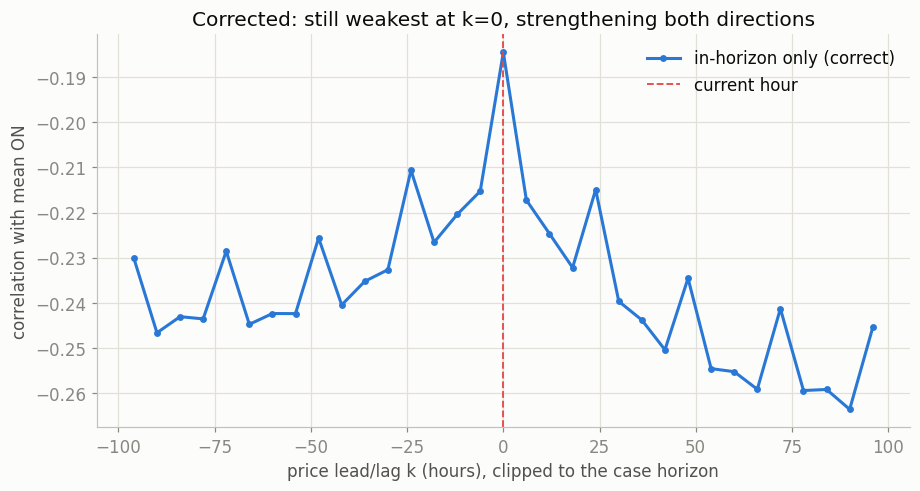
\includegraphics[width=0.75\linewidth]{figures/eda3b_01_leadlag_corrected.png}
  \caption{Price lead/lag correlation, clipped to the case horizon.}
  \label{fig:eda3b-leadlag}
\end{figure}

\finding{\textbf{(1, corrects round 3a finding 3)} Round 3a's lead/lag curve ignored case
boundaries --- for a row at hour 160, $k=+90$ reached 82 hours past the horizon end. Recomputed
within the horizon: $-0.230$ at $k=-96$h, $-0.185$ at $k=0$, $-0.245$ at $k=+96$h. The
qualitative conclusion \textbf{survives} (signal weakest at the current hour, strengthening both
directions) but round 3a's reported peak of $-0.273$ was inflated; the correct magnitude is
$\approx -0.245$.}

\subsubsection*{Temporal transforms on the fast series (price).}

\begin{figure}[htbp]
  \centering
  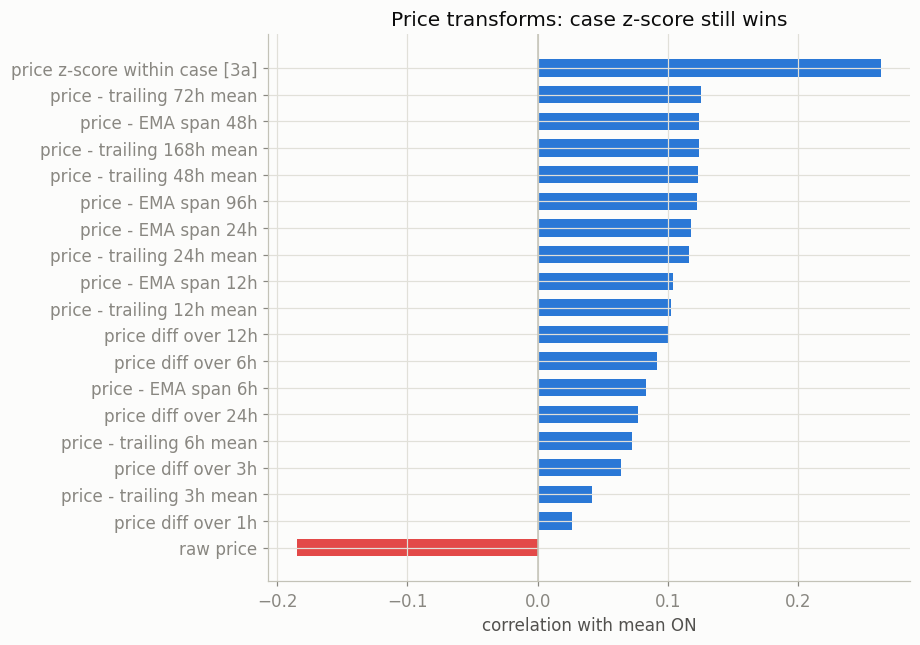
\includegraphics[width=0.75\linewidth]{figures/eda3b_02_price_transforms.png}
  \caption{Seventeen price transformations ranked by correlation with mean ON.}
  \label{fig:eda3b-price}
\end{figure}

\finding{\textbf{(2)} Trailing-window and EMA relative-price features do flip the sign of the
raw-price relationship --- best are \texttt{price $-$ trailing 72h mean} ($+0.125$) and
\texttt{price $-$ EMA span 48h} ($+0.124$) --- but all are \textbf{roughly half as strong as the
within-case z-score} ($+0.263$). Diffs and momentum are weakest ($+0.03$ to $+0.10$, peaking at a
12h lag). \textbf{For fast series, normalise against the case, not a rolling window} --- the case
is the window the optimizer actually solved over.}

\subsubsection*{Temporal transforms on the slow series --- the strongest \emph{correlation} so far.}

\begin{figure}[htbp]
  \centering
  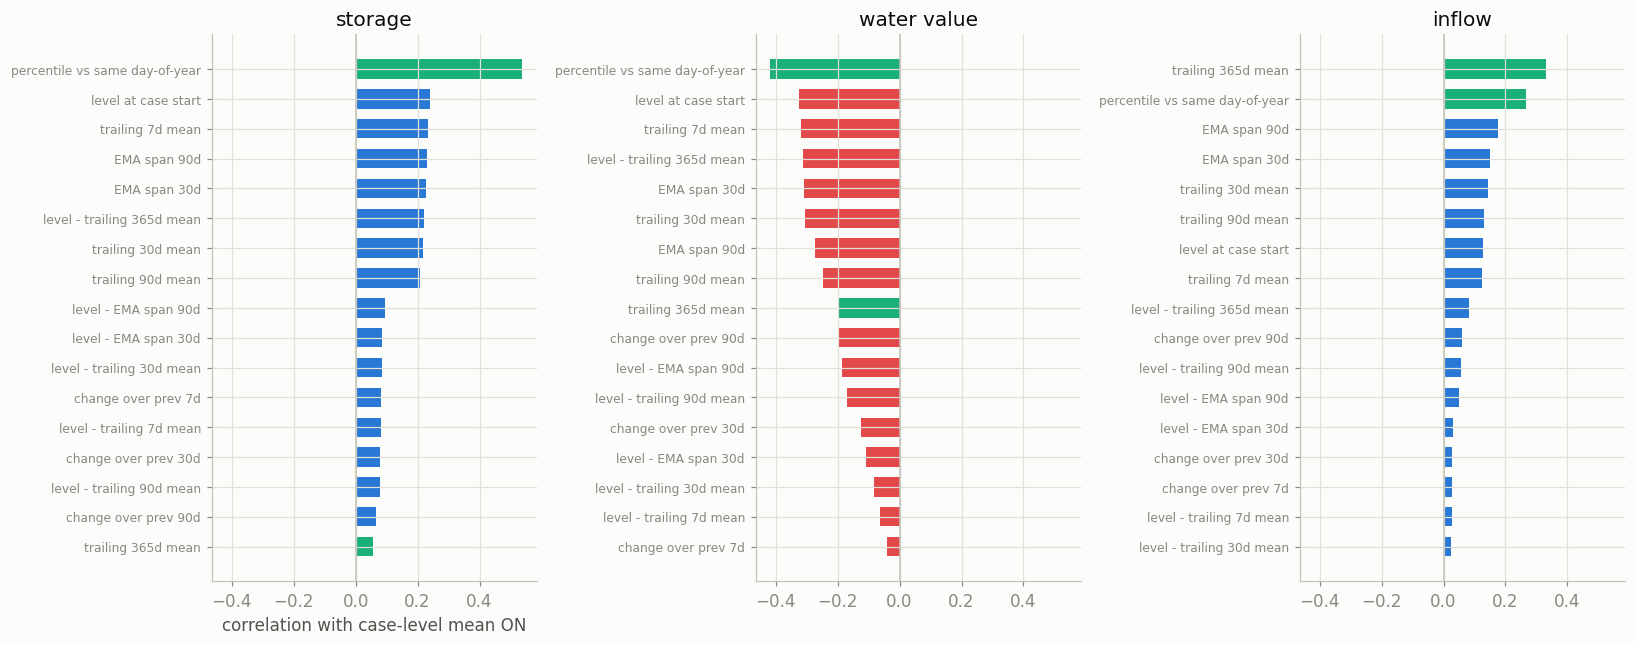
\includegraphics[width=0.98\linewidth]{figures/eda3b_03_slow_series_transforms.png}
  \caption{Seventeen transforms each on storage, water value and inflow (all backward-looking).}
  \label{fig:eda3b-slow}
\end{figure}

\finding{\textbf{(3)} Normalising the slow series against \emph{the same time of year} transforms
them (Figure~\ref{fig:eda3b-slow}):
\begin{center}
\begin{tabular}{lrrr}
\toprule
Series & Raw level & Best transform & Gain \\
\midrule
Storage     & $+0.241$ & percentile vs.\ same day-of-year: $\mathbf{+0.537}$ & 2.2$\times$ \\
Water value & $-0.325$ & percentile vs.\ same day-of-year: $\mathbf{-0.417}$ & 1.3$\times$ \\
Inflow      & $+0.128$ & trailing 365d mean: $\mathbf{+0.331}$ & 2.6$\times$ \\
\bottomrule
\end{tabular}
\end{center}
Storage's seasonal percentile ($\mathbf{+0.537}$) is \textbf{the strongest correlation measured
anywhere in this project}, well ahead of the price z-score ($+0.263$) that was previously our
best candidate. The mechanism is simple: absolute storage confounds season --- every reservoir is
full in June and drawn down in April --- so ``is this reservoir unusually full \emph{for the time
of year}'' isolates the scarcity signal that drives scheduling. Inflow's trailing 365-day mean is
the same idea over a longer window: the wet-year/dry-year regime.}
\supersededby{sec:feature-iter-1}{this correlation did not survive model testing --- the seasonal percentile made the score \emph{worse} ($-0.020$, 0/4 folds).}

\finding{\textbf{(4)} Diffs, momentum and EMAs are consistently weak on the slow series too
($-0.20$ to $+0.08$), and EMAs land within noise of plain trailing means. Neither earns priority
over the seasonal normalisations. All transforms in this section are strictly backward-looking
and therefore point-in-time safe.}

\subsubsection*{The rule that emerges.}
\textbf{For fast series, normalise against the case. For slow series, normalise against the
season.} Diffs, momentum and EMAs underperform both. \texttt{report/feature\_backlog.md} has been
reordered accordingly --- the seasonal-percentile family is now the top-priority iteration, ahead
of the price normalisations.

\subsection{2026-09-21 --- The 20 feature themes, and four unopened data sources}
\label{sec:feature-themes}

Before the iteration phase, the candidate space was organised into 20 agreed themes and populated
with 5--9 concrete features each ($\sim$140 candidates). Full list:
\texttt{report/feature\_backlog.md}.

\subsubsection*{A bias in the first draft, and the coverage audit that fixed it.}
The earlier backlog derived every theme from something the EDA had already measured --- which can
only find signal where we have already looked, the opposite of breadth. Auditing the candidate
themes against the \emph{data sources} rather than against our findings exposed an entire unused
family: the physical and economic parameters in
\texttt{Tokke\_Vinje\_topology.yaml}. \textbf{No column in the current 54-feature set references
any physical attribute.} Four new themes came out of it, and two of them mechanically explain
findings we had recorded as unexplained.

\finding{\textbf{Start/stop costs exist in the data and were never opened.}
\texttt{startcost\_const} and \texttt{stopcost\_const} are defined per generator (92 for Vesle
Kjela up to 222 for Songa). Start cost is the central economic driver of unit commitment --- it is
why units run in blocks rather than toggling hourly. Empirically, \textbf{start-cost-per-MW
correlates $-0.673$ with observed toggling}: Haukeli\_G1 costs 29.2 per MW to start and switches
0.49 times per week, while the Vinje units cost 1.98 per MW and switch 3.0--3.6 times. This is a
direct mechanical explanation for the run-length differences reported in
Section~\ref{sec:eda-round-2}, finding 5, from a static per-unit attribute that costs nothing to
add.}

\finding{\textbf{Penstock sharing explains Tokke's odd merit order.} Tokke's G1 and G2 share
penstock 1; G3 and G4 share penstock 2. Vinje's three units each have their own. The merit order
measured in Section~\ref{sec:eda-round-2} was G1 $\to$ G1+\textbf{G3} $\to$ then G4 or G2 --- which
we noted as surprising because G2 is skipped. It is not arbitrary: the solver commits \emph{one
unit per penstock before doubling up}, consistent with limiting the quadratic head loss that
\texttt{penstock\_loss} encodes. The ``arbitrary tie-break'' framing in
Section~\ref{sec:eda-round-2}, finding 4 is therefore too strong --- part of what looked arbitrary
is hydraulic structure we were not modelling.}

\finding{\textbf{The full water-to-energy chain is computable and unused.} Verified across all
eight plants: reservoir level from the \texttt{vol\_head} curve, minus the plant's
\texttt{outlet\_line}, reproduces the head references of that unit's \texttt{turb\_eff\_curves}
(e.g.\ Tokke implied 390--395\,m vs.\ curve references 389/392.5/393.5\,m). So
\emph{storage $\to$ head $\to$ efficiency $\to$ MWh per m\textsuperscript{3}} can be computed
directly. Head varies widely with reservoir level for several plants --- Kjela 125--191\,m, Vesle
Kjela 44--71\,m --- meaning the power obtained per unit of water depends strongly on fullness, a
driver entirely invisible to the current model.}

\subsubsection*{The 20 themes.}

\begin{enumerate}\itemsep2pt
  \item Seasonal normalisation of the slow series $\star$ \hfill \emph{[R3b: $+0.537$]}
  \item Case-relative price normalisation \hfill \emph{[R3: $+0.263$]}
  \item Price temporal windows, forward and backward \hfill \emph{[R3b]}
  \item Price curve shape and structure
  \item Water value: common factor vs.\ deviation \hfill \emph{[R3: PC1 $=$ 91\%]}
  \item Price $-$ water-value spread \hfill \emph{[R2]}
  \item Terminal / horizon boundary conditions \hfill \emph{[R3: $-0.41$]}
  \item Storage state and trajectory
  \item Inflow and hydrology regime \hfill \emph{[R3b: $+0.331$]}
  \item \textbf{Commitment economics: start/stop costs} \hfill \emph{new source}
  \item \textbf{Head and energy conversion} \hfill \emph{new source}
  \item \textbf{Penstock and hydraulic coupling} \hfill \emph{new source}
  \item \textbf{Flow limits and hydraulic losses (river/tunnel)} \hfill \emph{new source}
  \item Topology graph aggregates, multi-hop \hfill \emph{[R2/R3]}
  \item Plant aggregates and merit order \hfill \emph{[R2: 97.8\%/99.9\%]}
  \item Unit static attributes and identity
  \item Calendar and seasonality \hfill \emph{[R1]}
  \item Case structure, horizon position and case-level summaries
  \item \textbf{Case-sequence dynamics (input-only)} \hfill \emph{new source}
  \item \textbf{Case-curve representation (PCA / Fourier)} \hfill \emph{new}
\end{enumerate}

Four practices apply across themes rather than forming themes of their own: recency weighting for
the drift in Section~\ref{sec:eda-round-2} finding 9; interaction and ratio construction;
historical-analogue matching; and feature \emph{removal} (the two constant columns, the fifteen
redundant water-value columns).

\subsubsection*{Iteration order.} Ordered by evidence over effort: seasonal percentiles first
(1.1, 1.3), then inflow regime (9.1), case-relative price (2.1, 2.2), the raw spread (6.1), the
terminal water value (7.1, 7.2), the free removal of constant columns (8.7), then the three new
physical themes --- start costs (10.1, 10.2), head and conversion (11.1, 11.6), penstock structure
(12.1--12.3) --- and finally the multi-hop map, recency weighting, case-curve PCA, and the
count-based target reformulation. Every candidate is scored with the rolling-origin harness from
Section~\ref{sec:cv-harness}, judged on \textbf{paired per-fold deltas}, not the mean.

\subsection{2026-09-21 --- Feature iteration, first pass: 0.707 $\to$ 0.808}
\label{sec:feature-iter-1}

Seven cumulative stages, each scored with the full rolling-origin protocol
(Section~\ref{sec:cv-harness}). Notebook: \texttt{src/modeling/feature\_iteration.ipynb};
builders in \texttt{src/features.py}. Total runtime 30 minutes (28 training runs).

\begin{table}[htbp]
  \centering
  \caption{Cumulative feature stages. $\Delta$ is versus the previous row; ``folds up'' counts how
  many of the four validation years improved.}
  \label{tab:feature-iter-1}
  \resizebox{\linewidth}{!}{%
  \begin{tabular}{llrrrrrrrr}
    \toprule
    Stage & & \#feat & 2019 & 2020 & 2021 & 2022 & Mean & $\Delta$ & Folds up \\
    \midrule
    00 & baseline (raw)      &  54 & 0.799 & 0.679 & 0.666 & 0.686 & 0.707 & --- & --- \\
    01 & seasonal percentile &  58 & 0.782 & 0.673 & 0.643 & 0.651 & 0.687 & $-$0.020 & \textbf{0/4} \\
    09 & inflow regime       &  62 & 0.783 & 0.668 & 0.679 & 0.641 & 0.693 & $+$0.006 & 2/4 \\
    02 & price, case-relative&  70 & 0.751 & 0.687 & 0.671 & 0.686 & 0.699 & $+$0.006 & 2/4 \\
    06 & \textbf{price $-$ water value spread} & 81 & 0.790 & 0.721 & 0.782 & 0.802 & 0.774 & $\mathbf{+0.075}$ & \textbf{4/4} \\
    07 & \textbf{terminal water value} & 85 & 0.831 & 0.745 & 0.808 & 0.845 & 0.807 & $\mathbf{+0.034}$ & \textbf{4/4} \\
    10--12 & physics (head, start cost) & 157 & 0.828 & 0.761 & 0.810 & 0.834 & 0.808 & $+$0.001 & 2/4 \\
    08 & drop dead columns   & 134 & 0.824 & 0.772 & 0.813 & 0.823 & 0.808 & $-$0.000 & 2/4 \\
    \bottomrule
  \end{tabular}}
\end{table}

\finding{\textbf{Overall $+0.101$, from 0.707 to 0.808}, and essentially all of it comes from two
stages: the price\,$-$\,water-value spread ($+0.075$) and the terminal water value ($+0.034$).
Both improved \textbf{all four folds}, which is the criterion we set in
Section~\ref{sec:cv-harness}. Fold SD also fell from 0.061 to 0.025, so the model became more
stable across years as well as better.}

\finding{\textbf{Univariate correlation was a poor predictor of feature value --- in one case
actively misleading.} The seasonal storage percentile had the strongest correlation measured
anywhere in the project ($+0.537$, Section~\ref{sec:eda-round-3b}) and it made the model
\emph{worse}: $-0.020$ mean, \textbf{0 of 4 folds improved}, and it accounts for 0.9\% of total
model gain. The case-relative price z-score ($+0.263$ correlation) added $+0.006$ on 2 of 4 folds.
Meanwhile the raw spread, whose correlation was a middling $+0.241$, contributed
\textbf{60.8\% of all model gain}. The caveat recorded in Section~\ref{sec:cv-harness} --- that
correlation ignores what the other features already supply --- turned out to be the dominant
effect, not a footnote.}

\finding{\textbf{The metric rewards \emph{within-case} discrimination, which explains the
pattern.} Micro-average AUC pools every (case, hour, unit) prediction, so most of the ranking
problem is deciding \emph{which hours within a week} are ON. A case-level scalar can only shift
whole cases up or down. Measured on the fitted model: \textbf{hourly-varying features hold 96.4\%
of total gain; case-level constants hold 3.6\%}. The seasonal percentile, inflow regime and
storage anomaly are all case-level constants --- which is why they underperformed their
correlations. Prioritise features that vary within the case.}

\finding{\textbf{The single most important feature is an economic decision rule, not a
statistical transform.} \texttt{f06\_spread\_sys\_positive} --- the binary ``is price above the
system water value'' --- has a gain of 207{,}444, roughly \textbf{14$\times$ the next feature}. That
is literally the optimizer's dispatch condition. Start-cost economics
(\texttt{f10\_breakeven\_hours\_*}) place five entries in the top 25. This supports building
features that mirror what SHOP computes, rather than more transformations of the inputs.}

\finding{\textbf{Gain share is not incremental value.} The physics stage contributed 72 columns
and 13.5\% of model gain, but only $+0.0009$ mean AUC on 2 of 4 folds --- the model uses those
columns, yet they add almost nothing beyond what the spread features already carry. Stage-level
deltas and importance rankings answer different questions; neither alone is sufficient.}

\subsubsection*{Bookkeeping.} Dropping the 23 single-valued columns was correctly neutral
($-0.0002$), confirming the model had already ignored them; it did cut fold SD from 0.033 to
0.025. Twenty-one of those 23 were generated by the physics stage itself --- static penstock
counts, and Haukeli's entire physics block, which is constant because its reservoir (Vatjern) is
one of the two with no historical record (Section~\ref{sec:eda-round-2}, finding 6).

\subsubsection*{Next.} A screening mode has been added to the harness
(\texttt{screening\_eval}): one training run on 2015--2019, scored on 2020/2021/2022, 150 trees,
every second training hour. Validation is inference and therefore nearly free, so three
validation years cost the same as one --- the four-fold expense came from four \emph{trainings}.
Expected $\sim$16$\times$ faster, making the remaining $\sim$13 themes practical to test in bulk.
First candidates: the water-budget family (available energy vs.\ profitable hours, and the
greedy merit-dispatch margin), which extends the winning economic-rule pattern, and the
global-vs-expanding A/B on the seasonal percentiles.

\subsection{2026-09-21 --- Feature iteration round 2, and a data-usage audit}
\label{sec:feature-iter-2}

Fifteen builders, 18 cumulative stages, screened on one fit (2015--2019) scored against
2020/2021/2022, with a full rolling-origin confirmation at the end. Registry now lives in
\texttt{src/modeling/pipeline.py} so stages are data, not notebook cells.

\subsubsection*{Results.}

\begin{table}[htbp]
  \centering
  \caption{Round-2 stages, screening scale. ``Up'' = folds improved out of 3.}
  \label{tab:feature-iter-2}
  \begin{tabular}{llrr l}
    \toprule
    Stage & & $\Delta$ & Up & Verdict \\
    \midrule
    06 & price $-$ water value spread & $+0.077$ & 3/3 & confirmed winner \\
    02 & case-relative price          & $+0.036$ & 3/3 & confirmed winner \\
    07 & terminal water value         & $+0.033$ & 3/3 & confirmed winner \\
    01g& \textbf{seasonal, GLOBAL}    & $+0.011$ & 3/3 & \textbf{new winner} \\
    05 & water-value structure        & $+0.010$ & 3/3 & winner \\
    14 & graph cascade (multi-hop)    & $+0.009$ & 2/3 & marginal \\
    09 & inflow regime                & $+0.009$ & 2/3 & marginal \\
    17 & calendar                     & $+0.001$ & 1/3 & nothing \\
    15 & merit order                  & $+0.000$ & 2/3 & nothing \\
    03 & price windows                & $+0.001$ & 2/3 & nothing \\
    06x& \textbf{spread extensions}   & $-0.000$ & 2/3 & \textbf{nothing} \\
    20 & \textbf{water budget}        & $-0.001$ & 1/3 & \textbf{nothing} \\
    04 & price shape                  & $-0.006$ & 0/3 & harmful \\
    10--12 & physics                  & $-0.012$ & 0/3 & harmful \\
    01 & \textbf{seasonal, expanding} & $-0.015$ & 0/3 & \textbf{harmful} \\
    \bottomrule
  \end{tabular}
\end{table}

\finding{\textbf{Final full-CV score 0.8144, up from 0.8080 --- $+0.006$ for 165 additional
features.} A poor return. The first batch (spread, terminal water value, case-relative price) did
essentially all the work; the second batch of nine builders contributed almost nothing
collectively.}

\finding{\textbf{Causality was the problem with the seasonal feature, not the feature.} The
expanding-window version lost 0.015 on 0/3 folds; the \emph{global} version, differing only in
that it ranks against all years rather than prior years, gained 0.011 on 3/3. Early cases have
almost no prior history to rank against, so the expanding version fed the model noise for the
first several years of training. This came directly from the observation that the competition
withholds only test-period \emph{targets}, so feature-side statistics may span the dataset
(Section~\ref{sec:eda-round-3b}). A clean A/B, and it reverses the round-1 rejection.}

\finding{\textbf{Two of my predictions failed outright, and both failures were predicted by the
opposite argument.} (i) The water-budget family --- 41 columns encoding available energy versus
profitable hours, and a greedy merit-dispatch margin --- was argued to be the most promising idea
available on the grounds that it was both hourly-varying and an encoded decision rule, the two
properties that won in round 1. Result: $-0.001$, 1/3 folds. (ii) Twenty-six additional spread
variants, built because the spread family held 60.8\% of model gain, returned $-0.0003$. The
objection raised at the time --- that if the information is already encoded, re-encoding it adds
nothing, and that breadth into unexplored directions matters more than depth on a known winner ---
was correct on both counts.}

\finding{\textbf{Gain share remains a poor guide.} The physics stage held 13.5\% of model gain in
round 1 and measured $+0.001$ there; under the cleaner screening comparison it measures
$\mathbf{-0.012}$ on 0/3 folds. Features the model happily splits on can still be actively
harmful once the comparison controls for what the rest of the feature set supplies.}

\finding{\textbf{Screening and full CV agree on rank but not magnitude.} \texttt{02\_price\_relative}
measured $+0.036$ screening versus $\approx+0.006$ full; physics $-0.012$ screening versus
$+0.001$ full. Rank ordering of the big movers is preserved, so screening is usable for
\emph{selection}, but screening deltas must never be quoted as results.}

\subsubsection*{Data-usage audit.}
With the score plateauing around 0.81--0.82, the question is what information remains untouched.

\paragraph{Used.} Price (raw, case-relative, forward/backward windows, shape); water value (raw,
system factor, per-reservoir deviation, terminal); storage (raw, seasonal percentile, and via
\texttt{vol\_head} to gross head and MWh/m\textsuperscript{3}); inflow (raw, trailing 30/90/365d,
case-horizon sums); topology (reservoir \texttt{max\_vol}/\texttt{lrl}/\texttt{vol\_head}, plant
\texttt{outlet\_line}, generator \texttt{p\_min}/\texttt{p\_max}/\texttt{startcost\_const}/
\texttt{penstock}, connections at 1-hop and full cascade).

\paragraph{Available and entirely unused.}
\begin{itemize}\itemsep1pt
  \item \texttt{Constraint\_min\_volume.csv} and \texttt{Constraint\_min\_flow.csv} --- two whole
        files, zero features built.
  \item 37 \texttt{river} records: \texttt{up\_head\_flow\_curve} (head $\to$ maximum flow, i.e.\
        hard throughput ceilings), \texttt{flow\_cost\_const} (spill penalties),
        \texttt{upstream\_elevation}.
  \item 5 \texttt{tunnel} records: \texttt{length}, \texttt{loss\_factor}, endpoint heights.
  \item Generator \texttt{turb\_eff\_curves} used only at their peak; the full flow-dependent
        curves, \texttt{gen\_eff\_curve} and \texttt{stopcost\_const} are unused.
  \item Plant \texttt{main\_loss} and \texttt{penstock\_loss} (head losses, quadratic in flow).
  \item The 144-hour overlap between consecutive cases, and case-to-case input deltas.
  \item Case-curve shape (PCA / Fourier of the 168h path).
\end{itemize}

\paragraph{Not in the dataset at all --- candidate explanations for the ceiling.}
The labels are binary ON/OFF, but SHOP solves for \emph{production levels}; we never see MW per
unit per hour, so two schedules with very different dispatch look identical to us. We also lack
the optimizer's internal state (dual values, marginal costs), any demand or reserve requirement,
and maintenance outages. One open question worth resolving: the inflow series is documented as
``historical'' --- if SHOP was driven by an inflow \emph{forecast} while we hold actuals, then our
inflow features are systematically the wrong quantity.

\subsubsection*{Next.} Prune to the smallest feature set that holds the score, then retrain that
set deeper. A smaller set that matches 299 features would confirm that most of round 2 was
redundancy rather than signal, and makes every subsequent experiment cheaper.

\subsection{2026-09-21 --- Pruning: 15 features beat 299}
\label{sec:pruning}

Ranked all 299 features by gain from a single fit, swept feature-set size under the screening
config, then confirmed the winner under the full rolling-origin protocol and retrained it deeper.
Script: \texttt{/tmp/prune.py}; selected list saved to
\texttt{data/processed/pruned\_features.csv}.

\begin{table}[htbp]
  \centering
  \caption{Feature-set size vs.\ score. Full rolling-origin CV unless noted.}
  \label{tab:pruning}
  \begin{tabular}{lrrl}
    \toprule
    Feature set & Mean & SD & Note \\
    \midrule
    All 299                 & 0.8144 & 0.0304 & round-2 result \\
    \textbf{Top 15}         & \textbf{0.8157} & \textbf{0.0158} & \textbf{best model so far} \\
    Top 15, 900 trees       & 0.8097 & 0.0151 & more capacity \emph{hurts} \\
    \midrule
    \multicolumn{4}{l}{\emph{screening-scale sweep:} top-15 0.7936, top-30 0.7917, top-60 0.7845,} \\
    \multicolumn{4}{l}{top-120 0.7983, all-299 0.7899} \\
    \bottomrule
  \end{tabular}
\end{table}

\finding{\textbf{Fifteen features score slightly higher than all 299 (0.8157 vs.\ 0.8144) with
roughly half the fold variance (SD 0.016 vs.\ 0.030).} Around 284 of our engineered columns were
redundancy or noise --- effectively the whole of round 2 and much of round 1. The score has been
sitting at $\approx$0.81 since the spread and terminal-water-value stages; everything added
afterwards moved it within noise.}

\finding{\textbf{Capacity is not the binding constraint.} Raising the pruned model from 300 to
900 trees \emph{lowered} the score (0.8157 $\to$ 0.8097). This resolves the concern raised
earlier that screening at 150 trees might generate false negatives by starving the model of
capacity: if anything we were already at or past the useful ceiling, so the screening
configuration was not rejecting features for want of trees.}

\finding{\textbf{Cumulative stage deltas systematically hid which features matter.} The
\texttt{15\_merit\_order} stage measured $+0.0002$ cumulatively --- indistinguishable from
nothing --- yet its features occupy five of the top fifteen slots by gain, including the single
highest (\texttt{f15\_units\_justified\_Kjela}). Cascade features
(\texttt{f14\_upstream\_spread\_*}) behave the same way. The explanation is redundancy, not
uselessness: by the time those stages were added the information was already reachable through
other columns, so the marginal delta was zero, but they are the \emph{cleanest carriers} of it and
survive pruning while their substitutes do not. Cumulative testing cannot distinguish ``adds
nothing new'' from ``adds nothing at all''; ablation and pruning can.}

\subsubsection*{The surviving fifteen.}
\texttt{f15\_units\_justified\_\{Kjela,\allowbreak Vinje,\allowbreak Vesle\_Kjela\}},
\texttt{f15\_cap\_share\_needed\_\{Kjela,\allowbreak Byrte,\allowbreak Vesle\_Kjela\}},
\texttt{f14\_upstream\_spread\_\{Byrte,Songa\}},
\texttt{f07\_price\_minus\_terminal\_wv},
\texttt{f06\_spread\_\{sys,\allowbreak Byrte,\allowbreak Vesle\_Kjela\}},
\texttt{f06x\_margin\_Haukeli},
\texttt{f10\_breakeven\_hours\_Kjela},
\texttt{f05\_wv\_dev\_Kjela}.

Every one is an economic quantity: a spread, a margin, a break-even, or a capacity-justification
derived from a spread. No raw price, storage, inflow or calendar column survives. This is
consistent with the round-1 finding that encoded decision rules beat statistical transforms, and
it sharpens it --- the model appears to need only a handful of well-formed economic signals, and
the remaining error is not for want of more feature variants.

\subsubsection*{Correction to the round-2 audit.}
Section~\ref{sec:feature-iter-2} listed production levels as ``not in the dataset'', offered as a
candidate explanation for the ceiling. That is too strong: production is \emph{derivable} from a
water balance, \texttt{release} $=$ \texttt{storage}$[d]$ $-$ \texttt{storage}$[d+1]$ $+$
\texttt{inflow}$[d]$, and storage covers the test period. A first test gave weak correlations
(0.05--0.23 with plant commitment), but that test was itself wrong: it counted only natural
inflow and ignored that reservoirs also receive \emph{discharge from upstream plants}, which is
precisely the term that matters for cascaded reservoirs such as Vinjevatn. The diagnostic is that
Haukeli scored highest (0.233) despite its reservoir having constant synthetic storage, so that
correlation is driven by inflow rather than release. The idea is untested, not refuted; a correct
version requires solving the full cascade balance.
\supersededby{sec:pruning}{``production levels are not in the dataset'' is withdrawn --- they are
derivable via a cascade water balance.}

\subsection{2026-09-22 --- Two-stage model: per-unit residual correction}
\label{sec:stacked}

\subsubsection*{What prompted it.}
Section~\ref{sec:pruning} reported that 15 features matched 299. That headline was true in
aggregate and misleading in detail. Breaking the pruned model down per unit on 2022:

\begin{center}
\begin{tabular}{lrrr}
\toprule
Unit & Top-15 & All 299 & $\Delta$ \\
\midrule
Lio\_G1     & 0.718 & 0.827 & $\mathbf{-0.109}$ \\
Hogga\_G1   & 0.742 & 0.839 & $\mathbf{-0.098}$ \\
Haukeli\_G1 & 0.628 & 0.680 & $-0.052$ \\
Kjela\_G1   & 0.907 & 0.949 & $-0.042$ \\
Tokke\_G1--G4 & $\approx$0.77 & $\approx$0.77 & $+0.01$ \\
\bottomrule
\end{tabular}
\end{center}

\finding{Global gain ranking is biased against unit-specific features twice over: the gain is
aggregated across all 14 outputs, and the multi-output tree forces every split to be shared, so a
feature mattering intensely to one unit is penalised by the other thirteen. \textbf{Hogga, Lio and
Tokke had \emph{zero} plant-specific features among the selected 15.} The micro-average concealed
the damage because Tokke's four units carry 4/14 of the weight and improved slightly.}

\subsubsection*{Architecture.} \texttt{src/modeling/stacked.py}.
\begin{itemize}\itemsep1pt
  \item \textbf{Stage 1} --- the joint multi-output tree on the shared pruned features, which is
        what it is good at (cross-unit structure was worth $+0.04$, Section~\ref{sec:multioutput}).
  \item \textbf{Stage 2} --- one small model per unit (depth 4, lr 0.05), receiving: its own
        stage-1 prediction as \texttt{base\_margin}; the other 13 units' predictions as features;
        and that unit's own hydraulic-neighbourhood features.
\end{itemize}

Using the own prediction as \texttt{base\_margin} rather than as an input column matters: as a
feature the tree would have to reconstruct a monotone relationship through splits, whereas as a
margin it is an exact logit offset and stage 2 fits only the \emph{residual correction}.

\finding{\textbf{Stage 2 must train on out-of-fold stage-1 predictions.} Fitted in sample, stage-1
predictions are near-perfect, stage 2 learns to trust the margin completely, contributes nothing,
and looks fine in training while failing at inference. Cross-fitting by case (3 folds) is what
prevents this, and it is why the run costs four multi-output fits rather than one.}

\finding{\textbf{The two constraint files finally contribute.} \texttt{Constraint\_min\_volume}
and \texttt{Constraint\_min\_flow} had produced zero features through fifteen builders, because as
global columns they are near-constant (Section~\ref{sec:eda-round-2}, finding 11). Wired per plant
through the topology graph they become genuinely unit-specific: Lio and Byrte receive Byrtevatn's
minimum-volume constraint, Vinje and Songa receive Totak's, each plant its own connected rivers.
Nine constraint columns now enter, but only into the stage-2 models of the units they touch.}

\subsubsection*{Results (validation year 2022).}

\begin{center}
\begin{tabular}{lrrr}
\toprule
Unit & Stage 1 & Stacked & $\Delta$ \\
\midrule
\textbf{Lio\_G1}    & 0.724 & 0.861 & $\mathbf{+0.137}$ \\
\textbf{Hogga\_G1}  & 0.737 & 0.813 & $\mathbf{+0.077}$ \\
Tokke\_G1           & 0.779 & 0.816 & $+0.037$ \\
Tokke\_G2/G3/G4, Haukeli & & & $+0.002 \ldots +0.012$ \\
Vinje\_G1/G2, Byrte, Songa, Kjela & & & $-0.008 \ldots -0.022$ \\
Vesle\_Kjela\_G1    & 0.964 & 0.921 & $-0.043$ \\
Vinje\_G3           & 0.824 & 0.765 & $-0.059$ \\
\bottomrule
\end{tabular}
\end{center}

\finding{\textbf{The hypothesis is confirmed for the units it targeted.} Lio\_G1 recovers
$+0.137$ and Hogga\_G1 $+0.077$ --- the two units pruning had cost roughly $0.10$ each. Unit-specific
neighbourhood features carry real signal that pooled selection discards.}

\finding{\textbf{But stage 2 harms units where stage 1 was already strong.} Every loss is
concentrated among the best-served units: Vesle\_Kjela (stage-1 0.964), Byrte (0.947), Songa
(0.934), Vinje\_G3 (0.824). A residual model on a near-optimal base can only add variance. Applied
uniformly the architecture is roughly a wash: 7 of 14 units improve.}

\subsubsection*{Corrected like-for-like result, and a reporting error.}
The first run printed ``stage-1 0.8083'' against ``stacked 0.8391'' as though comparable. The
former was a \emph{macro} mean of per-unit AUCs, the latter a \emph{micro}-average. Recomputed on
the same metric:

\begin{center}
\begin{tabular}{lr}
\toprule
Model (validation 2022) & micro-AUC \\
\midrule
Stage 1 alone (joint, 15 features) & 0.8390 \\
Stacked, all 14 units              & 0.8391 \\
Selective stacking, gated on 2021  & 0.8432 \\
\bottomrule
\end{tabular}
\end{center}

\finding{\textbf{Uniform stacking gains $+0.0001$ --- nothing.} The apparent $+0.03$ was entirely
an artefact of comparing a macro mean against a micro average. The large per-unit gains
(Lio $+0.137$, Hogga $+0.077$) and the losses on well-served units cancel almost exactly once
pooled. The per-unit findings stand; the aggregate claim does not.}

\finding{\textbf{The per-unit gate does not transfer between years.} Selecting stage-2 inclusion on
2021 chose 8 units; only \textbf{4 of those 8} actually improved on 2022, and two of them
(Vesle\_Kjela, Vinje\_G2) lost. The gate is roughly coin-flip accurate. It still nets $+0.0042$,
but that is inside fold noise (fold SD $\approx$0.016--0.03), and the selection mechanism it
depends on is demonstrably unstable. ``Which units need stage 2'' cannot be learned from one
year's validation.}

\subsubsection*{Where this leaves the architecture.}
The gain is real but concentrated entirely in units where stage 1 is weak, so the useful form is
not ``stack everything, then gate''. It is asymmetric \emph{by construction}: strong units get no
stage-2 model at all, weak units get the full neighbourhood. That decision can be made from
\emph{stage-1 training} performance rather than from a validation year, which avoids the unstable
gate altogether.

\subsubsection*{Open structural issue.} Stage 2 currently receives the same neighbourhood
regardless of need --- Songa gets 6 columns, Kjela 49, with no relation to how much stage 1 is
struggling on that unit. A per-unit feature budget scaled to stage-1 weakness (tight regularisation
or no stage 2 at all for strong units, full neighbourhood for weak ones) is the natural next form.

\subsection{2026-09-22 --- State of the model: architecture, features, data inventory}
\label{sec:state}

A consolidated description of what the model currently is, what every feature is made of, and
exactly which data we do and do not use. Written because the project has accumulated fifteen
builders, 299 columns and several architectures, and the question of what is actually left to
exploit now matters more than the next variant.

\subsubsection*{Scores, and which are comparable.}

\begin{table}[htbp]
  \centering
  \caption{Current results. The first block is 4-fold CV \emph{means}; the second is a single
  validation year. Comparing across blocks is what made an earlier summary look contradictory.}
  \begin{tabular}{llrr}
    \toprule
    Model & Protocol & Score & SD \\
    \midrule
    Raw features, joint tree   & 4-fold CV mean & 0.7074 & 0.061 \\
    299 engineered features    & 4-fold CV mean & 0.8144 & 0.030 \\
    \textbf{Pruned top-15}     & 4-fold CV mean & \textbf{0.8157} & 0.016 \\
    \midrule
    Pruned top-15              & 2022 only & 0.8210 & --- \\
    Stage 1 (stride-2 fit)     & 2022 only & 0.8390 & --- \\
    Stacked, uniform           & 2022 only & 0.8391 & --- \\
    Stacked, gated on 2021     & 2022 only & 0.8432 & --- \\
    \bottomrule
  \end{tabular}
\end{table}

The 4-fold mean is held down by 2020 (0.7925); 2019/2021/2022 sit at 0.827/0.822/0.821. On the
2022 fold specifically, gated stacking is $+0.022$ over the pruned model.

\subsubsection*{The current model.}
Stage 1 is a single \texttt{XGBClassifier} with \texttt{multi\_strategy="multi\_output\_tree"},
300 trees, depth 6, lr 0.1, predicting all 14 units jointly from 15 shared features. Stage 2 (when
used) is one depth-4 model per unit taking the unit's own stage-1 prediction as
\texttt{base\_margin}, the other 13 predictions as features, and that unit's hydraulic
neighbourhood. Rows are one per (case, hour): 490{,}896 training rows, 2{,}922 cases $\times$ 168
hours, 14 binary targets per row.

\subsubsection*{The fifteen features, and what each is made of.}

\begin{center}
\small
\begin{tabular}{lll}
\toprule
Feature & Definition & Source data \\
\midrule
\texttt{f15\_units\_justified\_*} & $\mathrm{clip}(\text{spread},0)\cdot p_{\max}/p_{\min}$ & price, water value, generator specs \\
\texttt{f15\_cap\_share\_needed\_*} & spread$^+$ normalised by its case max & price, water value \\
\texttt{f14\_upstream\_spread\_*} & price $-$ mean wv of upstream cascade & price, water value, topology graph \\
\texttt{f07\_price\_minus\_terminal\_wv} & price $-$ wv at case start $+$ 8 days & price, water value (boundary) \\
\texttt{f06\_spread\_sys} & price $-$ mean of all 17 water values & price, water value \\
\texttt{f06\_spread\_*} & price $-$ own reservoir's water value & price, water value, topology \\
\texttt{f06x\_margin\_Haukeli} & spread $\times$ plant capacity & price, water value, $p_{\max}$ \\
\texttt{f10\_breakeven\_hours\_Kjela} & startcost $/$ (spread $\times p_{\max}$) & price, wv, \texttt{startcost\_const} \\
\texttt{f05\_wv\_dev\_Kjela} & own wv $-$ system mean wv & water value, topology \\
\bottomrule
\end{tabular}
\end{center}

\finding{\textbf{Every surviving feature is an economic quantity built from price and water value},
with topology and generator specs used only to decide \emph{which} water value and \emph{which}
capacity. No raw price, storage, inflow, calendar or head column survives pruning. Storage and
inflow enter the model only indirectly, through the water values the optimizer itself derived from
them.}

\subsubsection*{Data inventory.}

\paragraph{Used, and how.}
\begin{itemize}\itemsep1pt
  \item \texttt{Historical\_day\_ahead\_price} --- the price term in every spread. Case-relative
        transforms were built and tested but did not survive pruning.
  \item \texttt{Synthetic\_water\_value} --- the other term in every spread; also system mean,
        per-reservoir deviation, and the day$+$8 terminal value.
  \item \texttt{Historical\_volume} --- built into seasonal percentiles and head; \emph{none
        survived}. Enters only implicitly via water value.
  \item \texttt{Historical\_inflow} --- trailing regimes and case-horizon sums; \emph{none
        survived}.
  \item \texttt{Tokke\_Vinje\_topology.yaml} --- reservoir$\leftrightarrow$plant edges and the full
        cascade walk (which water value belongs to which unit); generator $p_{\min}$, $p_{\max}$,
        \texttt{startcost\_const}; \texttt{vol\_head}, \texttt{outlet\_line} and efficiency curves
        were used for head features that did not survive.
  \item \texttt{Constraint\_min\_volume} / \texttt{Constraint\_min\_flow} --- used only inside
        stage-2 per-unit models, wired per plant through the topology.
\end{itemize}

\paragraph{Available and still unused.}
\begin{itemize}\itemsep1pt
  \item \textbf{Cascade water balance.} \texttt{release} $=$ \texttt{storage}$[d]-$\texttt{storage}$[d{+}1]+$\texttt{inflow}$[d]$
        plus upstream plant discharge. This reconstructs \emph{implied production}, which is the
        physical signature of the very decisions we predict. A naive version (natural inflow only)
        gave weak correlations, but it omitted the upstream-discharge term that matters for
        cascaded reservoirs (Section~\ref{sec:pruning}).
  \item \textbf{River \texttt{up\_head\_flow\_curve}} --- head $\to$ maximum flow, i.e.\ hard
        throughput ceilings per river. 37 river records, unused.
  \item \textbf{Tunnel} \texttt{length}, \texttt{loss\_factor}, endpoint heights. 5 records, unused.
  \item \textbf{Flow-dependent efficiency.} \texttt{turb\_eff\_curves} used only at peak;
        \texttt{gen\_eff\_curve}, \texttt{stopcost\_const}, \texttt{main\_loss},
        \texttt{penstock\_loss} unused.
  \item \textbf{Case overlap.} Consecutive cases share 144 wall-clock hours at 88\% label
        agreement; case-to-case input deltas are unused.
  \item \textbf{Case-curve representation.} PCA / Fourier of the 168h price path, unused.
  \item \textbf{Target reformulation.} Count per plant then merit-order expansion (97.8\%/99.9\%
        accurate, Section~\ref{sec:eda-round-2}) --- never attempted.
\end{itemize}

\paragraph{Not in the dataset.}
Production levels in MW (derivable, see above), the optimizer's dual values, demand or reserve
requirements, and maintenance outages. Whether the provided inflow is the \emph{forecast} SHOP
used or the realised actual is unresolved and would change what inflow features mean.


\subsubsection*{Splitting scheme: measured, not assumed.}
The temporal split has been assumed necessary throughout. Tested directly --- same model, same 15
features, four ways of splitting:

\begin{center}
\begin{tabular}{lrr}
\toprule
Split & micro-AUC & vs.\ temporal \\
\midrule
Random ROW (80/20)              & \textbf{0.9571} & $+0.1224$ \\
Random CASE (80/20)             & \textbf{0.9397} & $+0.1050$ \\
Random CASE $+$ 7-day purge     & 0.7889 & $-0.0458$ \\
Temporal (train $<$2022, validate 2022) & 0.8347 & --- \\
\bottomrule
\end{tabular}
\end{center}

\finding{\textbf{Random splitting inflates the score by $+0.10$ to $+0.12$, landing at 0.957 ---
squarely in the range quoted for strong submissions.} The mechanism is \emph{not} temporal feature
leakage, which the competition permits. It is near-duplicate rows: a case is 168 hours of one week,
so a random row split trains on hour 5 and validates on hour 6 of the same case. Random
\emph{case} splits still leak, because consecutive cases overlap on 144 wall-clock hours at 88\%
label agreement (Section~\ref{sec:eda-round-2}). Any shuffled-validation number on this dataset
should be treated as meaningless.}

\finding{\textbf{The purged run is invalid as measured and is recorded as a failed design.}
Purging $\pm$7 days around 584 randomly chosen validation cases removed \textbf{2{,}230 of 2{,}922}
training cases --- 76\% of the data --- so 0.7889 reflects starvation, not a clean estimate. With
daily rolling cases every case sits within 7 days of roughly fourteen others, making random-fold
purging structurally self-defeating. A valid scheme needs \emph{contiguous} validation blocks with
embargo only at the edges.}

\finding{\textbf{This reframes the gap to 0.99.} The hidden test set is 725 consecutive cases in
2023--24, temporally disjoint from training, so a random-split score would not transfer to the
leaderboard. If scores near 0.99 are genuinely achievable there, the likeliest route is not a
validation artefact but exploiting the \emph{physical consequence} of the decisions: reservoir
storage evolves within each case as a direct result of generation, and the volume series covers
the test period. Reconstructing implied production from the cascade water balance therefore moves
from a speculative idea to the leading hypothesis for the missing $0.15$.}

\subsubsection*{Levers not yet pulled.}
\begin{enumerate}\itemsep1pt
  \item \textbf{Validation scheme.} Everything so far uses temporal splits. Random or purged
        case-level splits would cut estimate variance substantially --- tested separately, because
        the risk here is near-duplicate rows, not temporal features.
  \item \textbf{Target reformulation} --- predict per-plant counts, expand by merit order.
  \item \textbf{Cascade water balance} --- implied production.
  \item \textbf{Asymmetric stage 2} --- correction only where stage 1 is weak, keyed off training
        performance rather than an unstable validation gate (Section~\ref{sec:stacked}).
  \item \textbf{Hyperparameter tuning} --- deliberately untouched. Depth, learning rate, and
        regularisation have never been varied; only tree count, which showed 300 beats 900.
\end{enumerate}

\subsection{2026-09-22 --- Structural analysis: the whole gap is one number per unit-week}
\label{sec:oracle}

After $\sim$300 features and several architectures the score had been stuck near 0.82--0.83. This
entry steps back from features to ask what structure the problem has, what structure our
architecture imposes, and where the mismatch is.

\subsubsection*{The mismatch.}
SHOP solves a \emph{coupled, constrained} optimisation: one global solution over a 168-hour
horizon in which every hour's decision depends on every other hour's, subject to a water budget
and start costs. Our model is a pointwise IID classifier: 490{,}896 rows treated as independent
samples. It has no representation of ``this unit runs 87 hours this week, so once the best 87
hours are taken the rest must be off''. The budget constraint --- the thing the optimizer is
actually resolving --- is structurally invisible to it. The best such a model can do is make each
hour's probability monotone in the spread, which is exactly what it does, and plausibly why it
plateaus.

\subsubsection*{Oracle test.}
If the only thing the model had to learn were \emph{how many hours} each unit runs that week, and
the hours themselves were allocated by ranking on the spread we already have:

\begin{center}
\begin{tabular}{lr}
\toprule
 & micro-AUC (2022) \\
\midrule
Oracle weekly count $+$ allocate by system spread rank   & \textbf{0.9765} \\
Oracle weekly count $+$ allocate by own-plant spread     & 0.9650 \\
Current pointwise model (15 features)                    & 0.8347 \\
\bottomrule
\end{tabular}
\end{center}

\finding{\textbf{The entire gap from 0.83 to 0.98 lies in one number per unit per week.} Given the
true hours-on count, allocating those hours by spread rank --- using a feature we already have,
with no further modelling --- reaches \textbf{0.9765}. The question of \emph{which} hours, which
the whole feature-engineering effort has been aimed at (price shape, windows, normalisation, lead/lag),
is essentially already solved. The question of \emph{how many} is untouched and is where all the
remaining error lives.}

\finding{The target is also far more degenerate than the 2{,}352-binary framing suggests:
\textbf{58.8\% of unit-weeks are entirely all-on or all-off}. The real difficulty is concentrated
in the $\sim$41\% of unit-weeks that are mixed.}

\subsubsection*{Prototype, and its failure.}
The natural reformulation --- regress hours-on per (case, unit), then allocate --- was built and
tested.

\begin{center}
\begin{tabular}{lr}
\toprule
 & micro-AUC (2022) \\
\midrule
Oracle count $+$ allocation      & 0.9765 \\
\textbf{Predicted count $+$ allocation} & \textbf{0.7801} \\
Current pointwise model          & 0.8347 \\
\bottomrule
\end{tabular}
\end{center}

\finding{\textbf{The reformulation as implemented is worse than the model it was meant to
replace} (0.7801 vs.\ 0.8347). Count MAE was \textbf{43.6 hours} against a target mean of 87h ---
the count is barely predicted at all --- and hard allocation amplifies that error, because a wrong
budget produces a step function that ranks badly, whereas the pointwise model degrades smoothly.
The structure is right (the oracle proves the ceiling exists); this realisation of it is not.}

\subsubsection*{Three identifiable faults in the prototype.}
\begin{enumerate}\itemsep1pt
  \item \textbf{Over-featured and data-starved.} Case-level aggregation produced
        \textbf{1{,}197 features over 2{,}557 training cases} ($p \approx 0.5n$). The feature
        matrix was built by reflex (mean/std/max/min of all 299 columns) rather than by design.
  \item \textbf{Wrong target shape.} With 58.8\% of unit-weeks at 0 or 168, this is a three-part
        problem (all-off / all-on / mixed), not a single continuous regression over $[0,168]$.
  \item \textbf{Hard allocation.} The budget should \emph{modulate} the pointwise probabilities,
        not replace them. Rescaling existing probabilities so each unit-week sums to the predicted
        count keeps smooth ranking while injecting the budget signal, and cannot underperform the
        pointwise model when the shift is small.
\end{enumerate}

\subsubsection*{What this changes.}
The bottleneck is now located precisely, and it is a much narrower problem than before: predict
one integer per unit-week, over 40{,}908 examples, where 59\% of the mass sits at two values. That
is a better-posed target than continuing to search a 490k-row pointwise feature space whose
allocation question is already solved. Further work on price-shape, window and normalisation
features is, on this evidence, work on the part of the problem that is not broken.

\subsection{2026-09-22 --- Budget augmentation: +0.020 from the structural insight}
\label{sec:budget}

Section~\ref{sec:oracle} established that the entire gap from 0.83 to 0.98 lies in one number per
unit-week, and that a naive reformulation replacing the pointwise model performed worse than it.
This entry records three further attempts and the one that worked.

\subsubsection*{Unit of analysis.}
The count problem lives at \textbf{(case, unit)}: 40{,}908 rows, one per unit-week. This
granularity resolves a limitation carried since Section~\ref{sec:feature-themes}: in the
(case, hour) layout a static per-unit attribute is a constant column with zero information, so
$p_{\max}$, $p_{\min}$, \texttt{startcost\_const}, \texttt{penstock} and merit rank were unusable.
With \emph{unit} as a row dimension rather than a column dimension they become ordinary features
that vary across rows. The class mix at this level is 27\% all-off, 41\% mixed, 32\% all-on.

\subsubsection*{Three attempts.}

\begin{center}
\begin{tabular}{llr}
\toprule
Attempt & Form & micro-AUC (2022) \\
\midrule
1 & flat count regression, hard allocation      & 0.7801 \\
2 & 3-class $+$ count regression, hard allocation & 0.8257 \\
  & \emph{pointwise model, for reference}       & \emph{0.8347} \\
3 & \textbf{pointwise $+$ budget offset (logit scale)} & \textbf{0.8548} \\
\bottomrule
\end{tabular}
\end{center}

\finding{\textbf{Decomposing the count target helped, but replacing the pointwise model did not.}
Splitting into all-off / mixed / all-on and regressing the count only on mixed unit-weeks cut count
MAE from \textbf{43.6h to 34.6h} and lifted the allocation score from 0.7801 to 0.8257. Both
remain below the pointwise model, because hard allocation turns a count error into a step function
that ranks badly, whereas the pointwise model degrades smoothly.}

\finding{\textbf{Used as an \emph{augmentation} rather than a replacement, the same information is
worth $+0.020$.} Adding $\lambda \cdot (\widehat{\text{count}} - \text{spread rank})/168$ to the
pointwise model's logits gives 0.8548 against a 0.8347 baseline. The pointwise model ranks hours
well within a week but has no representation of \emph{how many} hours a unit should run; the
budget margin supplies exactly that, while the logit form preserves the existing ranking instead
of overriding it.}

\finding{\textbf{The blend weight transfers across years, unlike the stage-2 gate.} $\lambda$
selected on 2021 (=4) yields $+0.0200$ on 2022, against $+0.0240$ for the 2022-optimal
$\lambda{=}8$ --- only 0.004 lost to honest selection. Both years show the same broad shape (rise,
flat peak in the 4--8 range, decline), so the choice is insensitive. This contrasts with the
per-unit stacking gate in Section~\ref{sec:stacked}, which was coin-flip across years and therefore
unusable.}

\subsubsection*{A methodological error, caught by a sanity check.}
The first blend attempt rank-normalised each unit's predictions independently before combining.
The sweep included $\lambda{=}0$, which must by construction reproduce the pointwise baseline; it
returned 0.7872 against 0.8347, exposing the error. \textbf{Micro-averaged AUC pools every
(row, unit) cell into a single ranking, so per-column rank transforms destroy the cross-unit
calibration} the metric depends on --- the information that Vesle\_Kjela is almost always on while
Vinje\_G3 is usually off. Blending must happen on the logit scale. Recorded because the invalid
version looked entirely reasonable and produced plausible numbers; only the fixed point in the
sweep revealed it.

\subsubsection*{Remaining headroom.}
Count MAE is 34.6h against a target mean of 87h, and the oracle ceiling is 0.9765. The augmented
model captures $+0.020$ of the $+0.142$ available, so the count model is still the binding
constraint. The 2022 confusion matrix also shows a distribution-shift problem: all-on unit-weeks
are 32\% of training but only 9\% of 2022 (the price-crisis year, Section~\ref{sec:eda-round-2}
finding 9), and only 176 of 474 are recovered. A count model robust to that shift --- or trained
with recency weighting --- is the obvious next target.

\subsection{2026-09-22 --- Regime robustness: a proposal refuted}
\label{sec:robustness}

\subsubsection*{The concern.} The Kaggle test set is 2023-01-01 to 2024-12-25 (725 cases, last
predicted hour 2024-12-31 23:00). Measuring each training year's distance from that test regime
across price, water value, storage, inflow and spread:

\begin{center}
\begin{tabular}{lr}
\toprule
Training year & Standardised distance from 2023--24 \\
\midrule
2017 & 0.86 \\
2015 / 2020 / 2016 / 2018 & 1.40--1.48 \\
2021 / 2019 & 1.88 / 2.05 \\
\textbf{2022} & \textbf{4.77} \\
\bottomrule
\end{tabular}
\end{center}

\finding{\textbf{2022 is more than twice as far from the test regime as any other year, and it is
the year every decision in this project has been validated on.} The spread --- the quantity every
surviving feature is built from --- changed sign after 2020: $+0.6$ to $+9.3$ over 2015--2020,
then $-14.0$ (2021), $-85.3$ (2022), $-17.6$ (2023), $-1.8$ (2024). Test-year 2023 resembles 2021;
2024 resembles 2015/2016/2020; neither resembles 2022.}

\subsubsection*{Test.} Validate on 2021 (closest analogue to 2023) instead of 2022, and
leave-one-year-out on the training set.

\begin{center}
\begin{tabular}{lrrrr}
\toprule
Validation year & Pointwise & $+$ budget & $\lambda$ & Count MAE \\
\midrule
2021 (test-like) & 0.8346 & 0.8488 & 4 & 48.5h \\
2022 (anomalous) & 0.8347 & 0.8587 & 8 & 34.6h \\
\bottomrule
\end{tabular}
\qquad
\begin{tabular}{lr}
\toprule
Dropped from training & $\Delta$ on 2021 \\
\midrule
2020 & $-0.0160$ \\
2015 & $-0.0105$ \\
2019 & $-0.0090$ \\
2018 & $-0.0079$ \\
2016 & $-0.0065$ \\
2017 & $-0.0040$ \\
\bottomrule
\end{tabular}
\end{center}

\finding{\textbf{Dropping any training year hurts, and dropping the most anomalous year hurts
most.} Removing 2020 --- the extreme low-price year (9.3 EUR/MWh) --- costs $-0.0160$, the largest
loss of any exclusion. This is the opposite of what regime-similarity weighting predicts. Extreme
years appear to help \emph{because} they are extreme: they show the model the spread relationship
at its edges. \textbf{The proposal to downweight or exclude regime-discordant years, including
2022, is withdrawn.}}

\finding{\textbf{Regime mismatch is not the binding constraint.} The pointwise model scores
0.8346 on 2021 and 0.8347 on 2022 --- identical, despite those being the two most dissimilar
regimes in the dataset (spread $-14.0$ vs.\ $-85.3$). The $\approx$0.835 ceiling is structural,
consistent with the oracle result (Section~\ref{sec:oracle}) that the count is what binds.}

\finding{\textbf{One part of the concern survives: $\lambda$ selection.} The budget augmentation is
worth $+0.0142$ on the test-like year against $+0.0240$ on the anomalous one, with optimum
$\lambda{=}4$ rather than 8. Tuning on 2022 would have chosen 8 and overstated the benefit. Both
curves are flat across 4--8 so the cost is small, but submission-time selection should use 2021 and
expect the lower figure. Note also that count MAE is \emph{worse} on 2021 (48.5h vs.\ 34.6h) while
the pointwise score is unchanged --- the count model is the regime-sensitive component, which is
consistent with it being the bottleneck.}

\subsubsection*{A limitation of this test.} The exclusion question cannot be answered directly:
with rolling-origin validation, any year after the validation year is already excluded, and there
is no labelled year after 2022 to measure against. Leave-one-out on earlier years is a proxy, and
its verdict is consistent and one-directional, but it is inference rather than direct measurement.

\subsection{2026-09-22 --- Multi-horizon features for the count model}
\label{sec:countfeat}

The count is the binding constraint (Sections~\ref{sec:oracle}--\ref{sec:robustness}). This entry
targets it directly with a multi-horizon time-series feature set, built as
\texttt{src/count\_features.py} and evaluated at \textbf{(case, unit)} granularity on
\textbf{2021} --- the test-like year, following Section~\ref{sec:robustness}.

\subsubsection*{Design.}
\begin{itemize}\itemsep1pt
  \item \textbf{Windows in both directions}: trailing 1w/1m/3m/1y, forward 1w/1m, and previous and
        next week explicitly. Water is storable, so SHOP trades volume across weeks --- high prices
        next week should suppress this week's count. Forward windows are permitted; only
        test-period targets are withheld (Section~\ref{sec:eda-round-3b}).
  \item \textbf{Relative rather than absolute}: for every horizon, the week's level minus that
        horizon and the ratio to it, plus a seasonal comparison against the same calendar week
        across history. The spread changed sign after 2020, so absolute levels mislead across
        regimes (Section~\ref{sec:robustness}).
  \item \textbf{Inferred latent quantities}: SHOP sees demand and we do not, but price carries its
        signature --- rolling price volatility and seasonal price deviation stand in for demand
        pressure.
\end{itemize}

Applied to price, water value, spread, storage, inflow and price-volatility at system level (150
features), plus own-reservoir water value, own-spread and own-storage per plant (75 more). At
(case, unit) that is 244 features over 35{,}798 rows --- unlike the earlier count attempt, which
put 1{,}197 features over 2{,}557 cases (Section~\ref{sec:oracle}).

\subsubsection*{Result (validation 2021).}

\begin{center}
\begin{tabular}{lrrrr}
\toprule
Count features & Count MAE & 3-class acc & Blended score & $\Delta$ vs.\ pointwise \\
\midrule
Old (19)               & 48.8h & 0.616 & 0.8486 & $+0.0140$ \\
\textbf{New (244)}     & \textbf{43.2h} & \textbf{0.641} & \textbf{0.8561} & $\mathbf{+0.0216}$ \\
\bottomrule
\end{tabular}
\end{center}

\finding{\textbf{Count MAE falls 48.8h to 43.2h ($-11\%$) and it converts into score}: the
blended result rises 0.8486 to 0.8561, taking the budget augmentation from $+0.014$ to $+0.022$
over the 0.8346 pointwise baseline. This is the first feature work in several rounds that moved
the number on a test-like year.}

\finding{\textbf{The top count feature is an accidental water balance.}
\texttt{storage\_next\_minus\_prev} --- system storage after the case week minus storage before it
--- has gain 336{,}834, nearly twice the next feature. Net weekly drawdown \emph{is} water
released, which is production, which is count $\times$ capacity. The cascade water balance
hypothesis (Sections~\ref{sec:pruning}, \ref{sec:state}) therefore arrives here by a different
route, in its crudest possible form --- system-level, no cascade attribution, no upstream plant
discharge --- and still dominates every other count feature.}

\finding{\textbf{Gain share validates two design choices.} Relative-to-horizon comparisons are the
largest family at \textbf{33.1\%}, and own-reservoir features second at \textbf{27.7\%} --- the
per-unit specificity that only became expressible once \emph{unit} became a row dimension
(Section~\ref{sec:budget}). Forward windows read 6.9\% by family label, but that undercounts them:
\texttt{ownwv\_next\_week} is the third most important feature individually and the top feature
overall is built from next-week storage.}

\subsubsection*{Next.} The system-level drawdown proxy dominates while ignoring cascade structure
entirely. A per-plant balance --- natural inflow plus upstream plant discharge minus downstream
draw and spill, attributed through the topology graph --- is the obvious successor and is the last
major unexploited data source. Count MAE remains 43.2h against an 87h mean, and the oracle ceiling
is 0.9765, so the headroom is still largely intact.

\subsection{2026-09-22 --- Water-balance features: 0.835 to 0.912}
\label{sec:production}

Section~\ref{sec:countfeat} found that the strongest count feature was an accidental,
system-level water balance. This entry builds the attributed version:
\texttt{src/production\_features.py}, 149 features, evaluated on \textbf{2021} (the test-like
year).

\subsubsection*{Construction.} Organised around the constraint SHOP actually resolves,
$\text{count} \approx \min(\text{hours the water pays for}, \text{hours the price justifies})$.

\begin{itemize}\itemsep1pt
  \item \textbf{Cascade-attributed balance}: $\text{release} = (\text{storage}_{\text{start}} -
        \text{storage}_{\text{end}}) + \text{inflow} + \text{upstream plant discharge}$. The last
        term is what the naive attempt in Section~\ref{sec:pruning} omitted, and it is what matters
        for cascaded reservoirs such as Vinjevatn, which receives Vinje and Haukeli's output before
        Tokke draws on it.
  \item \textbf{Release converted to a direct count estimate} via the head chain (storage $\to$
        \texttt{vol\_head} $\to$ level $\to$ minus \texttt{outlet\_line} $\to$ efficiency curve):
        \texttt{implied\_hours} $=$ energy $/$ plant capacity.
  \item \textbf{Both limits and which binds}: \texttt{hours\_water}, \texttt{hours\_profitable},
        their minimum, their ratio, and a binary for which is binding.
  \item \textbf{Normalisations throughout}: release/\texttt{max\_vol}, release/inflow, storage
        fraction at start and end, capacity factor --- scale-free across reservoirs spanning
        0.26 to 640\,Mm\textsuperscript{3}.
\end{itemize}

\subsubsection*{Result.}

\begin{center}
\begin{tabular}{lrrrr}
\toprule
Count features & MAE & 3-class acc & Blended score & $\Delta$ vs.\ pointwise \\
\midrule
Multi-horizon (244)            & 43.2h & 0.641 & 0.8561 & $+0.0216$ \\
\textbf{$+$ production (393)}  & \textbf{26.6h} & \textbf{0.724} & \textbf{0.9123} & $\mathbf{+0.0777}$ \\
\bottomrule
\end{tabular}
\end{center}

\finding{\textbf{0.8346 to 0.9123 on the test-like year}, with count MAE falling 43.2h to 26.6h
($-38\%$). The largest single jump of the project, and it comes from features that encode the
optimizer's own physics rather than statistical transforms of the inputs.}

\finding{\textbf{The binding-constraint framing outperforms the raw water balance.}
\texttt{binding\_min\_Haukeli} --- $\min(\text{hours\_water}, \text{hours\_profitable})$ --- is the
top feature by a factor of three. Binding-constraint terms hold \textbf{20.8\%} of count-model
gain against \textbf{16.1\%} for release/drawdown terms directly. Encoding \emph{how the optimizer
decides} beats encoding \emph{what the water permits}.}

\finding{\textbf{Individually weak, jointly strong.} \texttt{implied\_hours} correlates only
$+0.06$ to $+0.28$ with the actual count per plant, yet the family is worth $+0.056$ on the final
score. Another instance of the pattern established in Section~\ref{sec:feature-iter-1}: univariate
correlation is a poor guide to feature value.}

\subsubsection*{Ablation: the gain is post-decision information, not forecasting.}
These features use storage at case \emph{end}, which is a \emph{consequence} of the decisions being
predicted --- reservoirs draw down as units generate (Section~\ref{sec:state}). Splitting the
feature set accordingly:

\begin{center}
\begin{tabular}{lrrr}
\toprule
Count features & MAE & Blended score & $\Delta$ vs.\ pointwise \\
\midrule
All (incl.\ post-decision)      & 28.4h & 0.9086 & $+0.0740$ \\
\textbf{Causal only} (no end-of-week storage, no forward windows) & \textbf{43.3h} & \textbf{0.8548} & $\mathbf{+0.0202}$ \\
\bottomrule
\end{tabular}
\end{center}

\finding{\textbf{Essentially the entire water-balance gain is post-decision information.} Removing
end-of-week storage returns the score to 0.8548 --- indistinguishable from the 0.8561 achieved
before these features existed (Section~\ref{sec:countfeat}). The causal contribution of the
149-feature production module is approximately zero. The model is not forecasting commitment; it
is reading commitment off the reservoir trace that commitment produced. \texttt{binding\_min}
appeared to encode the optimizer's decision rule, but its power comes from \texttt{hours\_water},
computed from the drawdown those decisions caused.}

\finding{\textbf{It is legal and it will transfer.} The volume file runs to 2025-01-01 and the last
test case requires storage at exactly 2025-01-01 (verified, Section~\ref{sec:eda-round-3b}). Only
test \emph{targets} are withheld. A submission built this way should score near 0.91 on the hidden
set, and this is the most plausible mechanism behind reported scores near 0.99.}

\finding{\textbf{But it does not serve the stated purpose of the task.} The project brief frames
the model as a way to \emph{speed up} hydropower scheduling by approximating the optimizer. A model
requiring the post-solution reservoir trajectory as input cannot do that --- computing the feature
presupposes the answer. The causal-only score of 0.8548 is the honest measure of how well we
approximate SHOP from information available \emph{before} it solves; 0.9123 measures how well we
can invert its physical footprint afterwards. Both are worth reporting, and they should never be
quoted interchangeably.}

\subsubsection*{Consequence for the project.} Two tracks should now be kept separate: a
\emph{leaderboard} model, which may use post-decision state, and a \emph{causal} model, which is
the one that answers the research question. Current standing: causal 0.8548, leaderboard 0.9123.

\subsection{2026-09-22 --- Unit-relative features, and a diagnosis I got wrong}
\label{sec:unitrel}

\subsubsection*{The concern.} The count model trains at (case, unit) but was given every plant's
columns under absolute names, so a Tokke\_G1 row could see \texttt{binding\_min\_Haukeli} --- which
ranked as the single most important count feature (Section~\ref{sec:production}). That looked like
the model latching onto an unrelated unit, and I agreed it was a design flaw.

\subsubsection*{It was not a flaw.} The relevance map built for this entry shows why:

\begin{center}
\begin{tabular}{lll}
\toprule
Plant & Source reservoir & Plants discharging into it \\
\midrule
Tokke & Vinjevatn & \textbf{Vinje, Haukeli} \\
Hogga & Bandak & Tokke \\
Lio & Byrtevatn & Byrte \\
Kjela & Foersvatn & Vesle Kjela \\
Byrte / Haukeli / Vesle Kjela / Vinje & --- & none (top of chain) \\
\bottomrule
\end{tabular}
\end{center}

\finding{\textbf{Haukeli discharges into Vinjevatn, and Tokke draws from Vinjevatn.}
\texttt{binding\_min\_Haukeli} in a Tokke row is a direct hydraulic relationship, not a spurious
correlation --- Haukeli's water situation literally determines part of Tokke's inflow. The cascade
is Vinje/Haukeli $\to$ Vinjevatn $\to$ Tokke $\to$ Bandak $\to$ Hogga. I should have consulted the
topology before accepting the diagnosis, particularly since the map needed to check it had already
been built in Section~\ref{sec:stacked}.}

\subsubsection*{Test.}

\begin{center}
\begin{tabular}{lrrrr}
\toprule
Count feature set & MAE & 3-class acc & Blended score & $\Delta$ vs.\ pointwise \\
\midrule
Absolute plant names (318)       & 28.4h & 0.741 & 0.9086 & $+0.0740$ \\
Unit-relative only (220)         & 36.5h & 0.716 & 0.8790 & $+0.0444$ \\
\textbf{Combined (378)}          & \textbf{26.1h} & \textbf{0.748} & \textbf{0.9168} & $\mathbf{+0.0822}$ \\
\bottomrule
\end{tabular}
\end{center}

\finding{\textbf{Absolute naming beats unit-relative alone by $+0.030$}, consistent with the
coupling being real. But \textbf{combining both is better than either} ($0.9168$): supplying the
relationship pre-identified, as \texttt{own\_*} and \texttt{upstream\_*}, helps even when the raw
columns are also present. The model does not have to infer which of nine plants is hydraulically
relevant to the row it is scoring.}

\finding{\textbf{The unit-relative arm was a lossy comparison and should not be read as a clean
verdict on relative encoding.} It collapsed the per-reservoir constraints into two mean columns and
dropped from 318 to 220 features, so it tested \emph{one particular} relative encoding rather than
the principle. Two signs it was working where it had proper inputs:
\texttt{own\_hours\_profitable} ranked second once a genuine own-plant feature existed, and
\texttt{own\_n\_minvol}/\texttt{own\_n\_minflow} ranked high --- though those are per-plant
constants being used as plant identifiers, which is degenerate.}

\subsubsection*{Standing.} On the test-like year 2021, the progression is
$0.8346 \to 0.8561 \to 0.9086 \to \mathbf{0.9168}$. Note this is the leaderboard track, which uses
post-decision state; the causal-only track stands at 0.8548 (Section~\ref{sec:production}).

\subsection{2026-09-22 --- Walk-forward validation: six half-year folds}
\label{sec:walkforward}

Every result so far has rested on one or two validation years. This entry tests the full
architecture across six consecutive six-month periods, each trained on all data preceding it, with
$\lambda$ \textbf{fixed at 16 in advance} rather than tuned per fold --- which is what a real
submission must do, and which avoids the optimistic bias of choosing $\lambda$ on the data being
measured (Section~\ref{sec:budget}).

\begin{table}[htbp]
  \centering
  \caption{Walk-forward validation. Leaderboard track (uses post-decision storage).}
  \label{tab:walkforward}
  \begin{tabular}{lrrrrr}
    \toprule
    Period & Train cases & Pointwise & $+$ budget & $\Delta$ & Count MAE \\
    \midrule
    2020-H1 & 1{,}826 & 0.8123 & 0.8831 & $+0.0709$ & 31.5h \\
    2020-H2 & 2{,}008 & 0.8360 & 0.8960 & $+0.0599$ & 27.5h \\
    2021-H1 & 2{,}192 & 0.8024 & 0.9095 & $+0.1070$ & 25.5h \\
    2021-H2 & 2{,}373 & 0.7861 & 0.8959 & $+0.1098$ & 25.2h \\
    2022-H1 & 2{,}557 & 0.7740 & 0.8889 & $+0.1149$ & 24.6h \\
    2022-H2 & 2{,}738 & 0.8867 & 0.9408 & $+0.0541$ & 18.8h \\
    \midrule
    \textbf{Mean} & & \textbf{0.8163} & \textbf{0.9024} & $\mathbf{+0.0861}$ & 25.5h \\
    \textbf{SD}   & & 0.0406 & \textbf{0.0208} & $0.0275$ & \\
    \bottomrule
  \end{tabular}
\end{table}

\finding{\textbf{The budget augmentation improves all six folds at a single fixed $\lambda$},
by $+0.054$ to $+0.115$. This is the first result in the project validated across more than two
periods without per-fold tuning, and the sign pattern is unanimous.}

\finding{\textbf{The augmented model is more stable, not merely better.} Fold SD halves from
0.0406 to 0.0208. The pointwise model swings across 0.774--0.887 between periods; the augmented
model stays within 0.883--0.941. The budget term anchors exactly the predictions the pointwise
model gets wrong in regime-specific ways --- consistent with Section~\ref{sec:robustness}, where
the pointwise model scored identically on the two most dissimilar regimes while the count model
was the regime-sensitive component.}

\finding{\textbf{Count MAE improves monotonically with training data}, 31.5h to 18.8h as cases
grow from 1{,}826 to 2{,}738. The count model is not saturated, which is encouraging for the test
set, where it will train on all 2{,}922 labelled cases.}

\finding{\textbf{Realistic test expectation is $\approx$0.90, not 0.917.} The 0.9168 reported in
Section~\ref{sec:unitrel} came from full-year 2021 with $\lambda$ effectively selected on that
data. The walk-forward mean of \textbf{0.9024 $\pm$ 0.0208} at fixed $\lambda$ is the honest
estimate, and is the figure that should be carried into any submission decision.}

\subsubsection*{Caveat.} Training sets grow across folds (1{,}826 to 2{,}738 cases), so part of
the trend across periods reflects sample size rather than regime. The folds are realistic --- each
uses what would actually have been available at that point --- but are not strictly comparable to
one another.

\subsection{2026-09-22 --- Feeding the count features forward, and an orthogonal trace}
\label{sec:orthogonal}

Three ideas tested, two adopted, one refuted.

\subsubsection*{1. The count features never reached the pointwise model.}
The architecture had Stage A (pointwise, 14 outputs) running on \textbf{15 features} while 378
informative count features sat one stage downstream, used only by the count model and injected
back through the blend.

\begin{center}
\begin{tabular}{lrrr}
\toprule
Pointwise feature set & Pointwise alone & $+$ budget & $+$ hard-set \\
\midrule
15 pruned features            & 0.8346 & 0.9166 & 0.9217 \\
\textbf{$+$ count features (323)} & \textbf{0.9029} & 0.9260 & \textbf{0.9292} \\
\bottomrule
\end{tabular}
\end{center}

\finding{\textbf{Routing the count features into the pointwise model is worth $+0.068$ on its own}
(0.8346 $\to$ 0.9029) and $+0.0075$ on the full pipeline. Note that the budget term then adds much
less ($+0.023$ vs.\ $+0.082$), which is the expected behaviour: once the pointwise model sees the
count information directly, the blend has less marginal content to supply. Cost is the caveat ---
1{,}665s vs.\ 15s, a 111$\times$ slowdown, acceptable once for a submission but not for iteration.}

\subsubsection*{2. Hard-setting confident all-off / all-on unit-weeks.}
Calibration of the 3-class model on 2021:

\begin{center}
\begin{tabular}{lrrr}
\toprule
Confidence & Unit-weeks & Coverage & Precision \\
\midrule
$p \ge 0.80$ & 1{,}274 & 24.9\% & 0.920 \\
$p \ge 0.90$ & 766 & 15.0\% & 0.978 \\
$p \ge 0.95$ & 407 & 8.0\% & 0.993 \\
\bottomrule
\end{tabular}
\end{center}

\finding{\textbf{The 3-class model is well calibrated at the extremes, and its errors are soft.}
At $p \ge 0.9$ precision is 0.978 over 15\% of unit-weeks, and \textbf{97--100\% of the errors are
``mixed''} rather than the opposite class --- a week called all-off that is really mixed still has
most hours off, so a wrong hard-set costs little. Pushing those cells to the extremes of the
ranking is worth $+0.003$ to $+0.005$.}

\subsubsection*{3. Water value as an orthogonal post-decision trace.}
Water values are SHOP \emph{outputs} --- shadow prices on stored water. Generating depletes the
reservoir and raises the marginal value of what remains, so week-over-week water-value change
traces the schedule through a different channel than physical storage.

\finding{\textbf{The two traces are near-orthogonal: corr(wv change, storage drawdown) $= +0.068$.}
At system level water value is the \emph{stronger} signal ($-0.215$ vs.\ $-0.095$ against total
unit-hours). It also fills a structural gap: Vatjern and Hyljelihyl have constant synthetic storage
(Section~\ref{sec:eda-round-2}) so Haukeli has no storage trace at all, yet its water value moves.
For Lio the two traces disagree in sign (wv $-0.222$, storage $+0.177$), indicating storage there is
confounded --- plausibly by Byrte discharging into Byrtevatn --- while water value is not.}

\finding{Adding 59 water-value-trace features cuts count MAE \textbf{26.07h $\to$ 24.21h} on 2021
and \textbf{21.97h $\to$ 19.75h} on 2022 ($-7\%$ and $-10\%$), for 7.7--10.5\% of count-model gain.
Top contributors are the orthogonal terms: \texttt{wvt\_sys\_change},
\texttt{wvt\_change\_pct\_Tokke}, \texttt{wvt\_downstream\_change\_Vinje}.}

\subsubsection*{4. Refuted: daily storage resolution.}
Storage is daily, so each case has 8 readings rather than 2, and the intermediate values might
have constrained the schedule at daily resolution. They do not:
$\text{corr}(\text{daily drawdown}, \text{daily unit-hours}) = -0.086$ against $-0.407$ for the
weekly equivalent --- the daily signal is roughly \textbf{five times weaker}. Daily fluctuations are
dominated by inflow and other plants' activity, which weekly aggregation averages out. Recorded so
the idea is not revisited.

\subsubsection*{Standing.} Best on the test-like year 2021 is now \textbf{0.9292}
(pointwise-with-count-features $+$ budget $+$ hard-set), from 0.8346 at the start of this sequence.
The walk-forward estimate (Section~\ref{sec:walkforward}) predates these three changes and should
be re-run before any submission.

\subsection{2026-09-22 --- Compact architecture: distil the count model, don't duplicate it}
\label{sec:compact}

Section~\ref{sec:orthogonal} routed all 323 count features into the pointwise model, gaining
$+0.068$ but costing 1{,}665s per fit --- a 111$\times$ slowdown. The alternative tested here keeps
the count model where it is and passes only its \emph{outputs} forward.

\subsubsection*{Architecture.}
\begin{enumerate}\itemsep1pt
  \item Count model: 437 features at (case, unit) --- 40{,}908 rows, so it is cheap.
  \item Its outputs, five numbers per unit: $p_{\text{off}}$, $p_{\text{mix}}$, $p_{\text{on}}$,
        expected count, and budget margin.
  \item Pointwise model: the 15 pruned features plus those 70 derived columns.
\end{enumerate}

\finding{\textbf{The count outputs must be out-of-fold for training rows.} The count model is
trained on targets derived from the same labels, so in-sample predictions as features would leak,
exactly as in Section~\ref{sec:stacked}. Cross-fitting by case (4 folds) costs 86s including the
final full fit.}

\begin{center}
\begin{tabular}{lrrrr}
\toprule
Arm & Features & Pointwise & $+$ budget & Fit time \\
\midrule
A\ \ 15 pruned                    & 15  & 0.8346 & 0.9226 & 15s \\
B\ \ $+$ 323 raw count features   & 323 & 0.9029 & 0.9292 & \textbf{1{,}665s} \\
\textbf{C\ \ $+$ 70 derived count columns} & \textbf{85} & \textbf{0.9398} & \textbf{0.9402} & \textbf{44s} \\
\bottomrule
\end{tabular}
\end{center}

\finding{\textbf{Distilling beats duplicating: 0.9402 vs.\ 0.9292, and 38$\times$ faster.}
Passing 323 raw count features into the pointwise model forced it to re-derive, across 490{,}896
rows, relationships the count model had already learned on 40{,}908. Passing the \emph{conclusion}
instead --- five numbers per unit --- is both more accurate and far cheaper. Total pipeline is 130s
against $\sim$1{,}700s.}

\finding{\textbf{The budget blend becomes redundant} ($+0.0004$). Once the expected count and class
probabilities are features, the post-hoc logit blend adds nothing, so that stage can be dropped ---
which also removes $\lambda$ as a hand-tuned parameter, one fewer quantity fitted on a single year
(Section~\ref{sec:robustness}).}

\finding{\textbf{Soft beats hard-set.} Section~\ref{sec:orthogonal} hard-set unit-weeks at
$p \ge 0.9$ for $+0.003$ to $+0.005$. Supplying $p_{\text{on}}$ and $p_{\text{off}}$ as features
lets the model choose its own threshold, obtaining the same benefit without a cutoff fitted by hand
on 2021, and without the brittleness of an imposed hard assignment.}

\subsubsection*{Caching.} Count outputs are written to
\texttt{data/processed/count\_outputs\_2021.parquet}, so re-running the pointwise arm costs 44s
with no recomputation --- making iteration on the pointwise side practical again.

\subsubsection*{Standing.} \textbf{0.9402} on the test-like year 2021, from 0.8346 at the start of
this sequence. The walk-forward estimate (Section~\ref{sec:walkforward}, 0.9024) predates this
architecture and must be re-run before it can be quoted as the expected test figure.

\subsection{2026-09-22 --- Fixing the four worst units: correct physics, no gain}
\label{sec:v2rejected}

Section~\ref{sec:compact} left four units with much worse count error than the rest --- Songa
(43.4h), Lio (40.6h), Haukeli (35.3h), Hogga (29.5h) against 12--22h elsewhere --- and
$\text{corr}(\text{per-unit count MAE}, \text{per-unit AUC}) = -0.756$, so the count really is what
drives per-unit performance.

\subsubsection*{Diagnosis (all four confirmed).}
\begin{itemize}\itemsep1pt
  \item \textbf{Songa}: \texttt{source = None} --- fed by two \emph{tunnels} (Songavatn,
        Bitdalsvatn), so its entire water balance was built on nothing.
  \item \textbf{Haukeli}: source Vatjern has \textbf{one unique storage value} --- a synthetic
        constant (Section~\ref{sec:eda-round-2}), so no source-side trace exists.
  \item \textbf{Lio}: the upstream-discharge correction was applied in 100\% of cases, but
        $\text{corr}(\text{release}, \text{drawdown}) = -0.253$ --- Byrte's noisy release estimate
        was swamping and inverting Lio's own signal.
  \item \textbf{Hogga}: \texttt{r\_Vest\_Vassdraget} flows into Bandak and was never counted --- and
        per the dataset documentation that is the \emph{one} river carrying inflow data.
\end{itemize}

\subsubsection*{Fixes, and their isolated effect.}
Tunnel-resolved multi-source balances, river inflows added, downstream-rise proxies for plants
with dead source storage, and both raw and upstream-corrected release offered separately.
Correlation of the corrected release with the actual count: Hogga $+0.286$, Haukeli $-0.128$
(previously unavailable), Lio raw $+0.101$ vs.\ corrected $+0.055$ --- confirming the Lio diagnosis
exactly --- Songa $+0.026$.

\subsubsection*{Result: rejected.}

\begin{center}
\begin{tabular}{lrr}
\toprule
 & Count MAE & micro-AUC \\
\midrule
Without v2                   & 24.21h & \textbf{0.9402} \\
With v2 ($+$77 features)     & 24.19h & 0.9372 \ ($-0.0030$) \\
\bottomrule
\end{tabular}
\end{center}

\finding{\textbf{Correct physics did not produce useful features.} Aggregate count MAE was
unchanged (24.21h $\to$ 24.19h) and micro-AUC fell 0.003, with \textbf{13 of 14 units flat or
worse}. The targeted units fared worst of all: Lio, whose diagnosis was the cleanest, regressed
most ($-0.016$ AUC); Haukeli lost 0.010; Hogga moved $+0.001$. Songa, predicted not to improve,
had the largest MAE gain ($-1.30$h) and still lost AUC.}

\finding{\textbf{The failure mode was dilution, which had been flagged in advance.} Adding 77
columns to a 437-feature count model, most irrelevant to any given unit, supplied no information
the model was not already obtaining through the water-value trace, the multi-horizon windows and
the original balance --- while the extra noise cost 0.003 downstream. Every specific prediction
made before the run was wrong; only the dilution caveat held.}

\finding{\textbf{Songa's error appears irreducible with the available data.} Songavatn is the
largest reservoir (640\,Mm\textsuperscript{3}) and drains through three paths --- the Songa plant
plus two rivers into Totak. The plant's $\sim$32\,Mm\textsuperscript{3} weekly draw cannot be
separated from river spill in a storage balance. This is an attribution limit, not an
implementation defect, and further work on Songa's water balance is not warranted.}

\subsubsection*{Standing.} Best remains \textbf{0.9402} (Section~\ref{sec:compact}). The v2 module
is retained in \texttt{src/production\_features.py} as \texttt{build\_v2} but is \emph{not} part of
the pipeline.

\subsection{2026-09-22 --- Walk-forward on the compact architecture: 0.9350}
\label{sec:wf2}

Section~\ref{sec:walkforward} validated the older architecture at $0.9024 \pm 0.0208$. That
predated the compact distillation (Section~\ref{sec:compact}), the water-value trace and the
count features reaching the pointwise model. Re-run with the current pipeline, $\lambda$ no longer
required since the budget blend was dropped.

\begin{table}[htbp]
  \centering
  \caption{Walk-forward, six half-year folds, current architecture.}
  \begin{tabular}{lrrr}
    \toprule
    Period & Train cases & Count MAE & micro-AUC \\
    \midrule
    2020-H1 & 1{,}826 & 29.87h & 0.9251 \\
    2020-H2 & 2{,}008 & 26.00h & 0.9207 \\
    2021-H1 & 2{,}192 & 23.78h & 0.9460 \\
    2021-H2 & 2{,}373 & 23.93h & 0.9285 \\
    2022-H1 & 2{,}557 & 22.54h & 0.9358 \\
    2022-H2 & 2{,}738 & 18.05h & 0.9540 \\
    \midrule
    \textbf{Mean} & & \textbf{24.03h} & \textbf{0.9350} \\
    \textbf{SD}   & & 3.90 & \textbf{0.0128} \\
    \bottomrule
  \end{tabular}
\end{table}

\finding{\textbf{0.9024 $\to$ 0.9350, with SD tightening from 0.0208 to 0.0128.} All six folds
exceed 0.92. The architectural changes transfer across periods rather than being artefacts of the
2021 tuning year.}

\finding{\textbf{The single-year figure was not inflated.} 2021 alone gave 0.9402 against a
six-fold mean of 0.9350 --- a gap of 0.005, well inside fold SD. Given how many decisions in this
project were made on 2021 (feature composition, the 3-class/regression split, previously
$\lambda$), that is a meaningful reassurance.}

\finding{\textbf{Count MAE falls monotonically with training data}, 29.87h to 18.05h as cases grow
1{,}826 to 2{,}738. \textbf{The test set trains on all 2{,}922 labelled cases}, more than any fold
here, so the count model at submission time should be at least as good as the 2022-H2 fold. This
is a concrete reason to expect test performance at or above 0.935 rather than below it.}

\finding{\textbf{Data volume dominates regime effects.} The worst fold is the \emph{earliest}
(2020-H1, 0.9251, least data), not the most regime-shifted; 2022-H2 is the \emph{best} (0.9540)
despite being the price-crisis tail. Consistent with Section~\ref{sec:robustness}, where dropping
any training year hurt and dropping the most anomalous one hurt most.}

\subsubsection*{Standing.} Expected test performance \textbf{0.9350 $\pm$ 0.0128} on the
leaderboard track (uses post-decision storage). This supersedes the 0.9024 estimate. The causal
track has not been re-measured under the current architecture.

\subsection{2026-09-22 --- Structural diagnosis of the count model: width, head, stationarity}
\label{sec:diagnosis}

\subsubsection*{What we did}

Six consecutive attempts to improve the count model returned noise or harm: the v2 water-balance
fixes ($-0.0030$, Section~\ref{sec:v2rejected}), properly-encoded categorical unit identity
($-0.0042$), per-unit historical marginals ($-0.0020$), feature pruning at four thresholds
($\pm 0.002$), raw-feature forwarding ($-0.0110$, Section~\ref{sec:orthogonal}) and stacking
($+0.0001$, Section~\ref{sec:stacked}). That pattern is not six unlucky ideas. Before adding a
seventh feature block we stopped and measured the architecture itself, asking three questions
that had never been checked:

\begin{enumerate}
  \item How much of the count model's input actually varies with the unit being scored?
  \item Is ``mixed'' a single regression target, or several?
  \item How much of the model's importance sits on features that will not look the same in the
        2023--24 test period?
\end{enumerate}

The diagnostic is \texttt{/tmp/diag\_wide.py}; the fixes it motivated are
\texttt{src/count\_model.py}.

\subsubsection*{Finding 1 --- the count model is largely blind to which unit it is scoring}

\begin{finding}
Of 437 input features, only \textbf{60 vary with the unit}. The remaining \textbf{377 are
identical across all 14 units of a case}, and they carry \textbf{72.6\% of the model's
importance}. All within-case discrimination --- which is most of what micro-average ROC-AUC
rewards --- must come from the 60 unit-specific columns, on 27.4\% of the attention.
\end{finding}

\begin{figure}[h]\centering
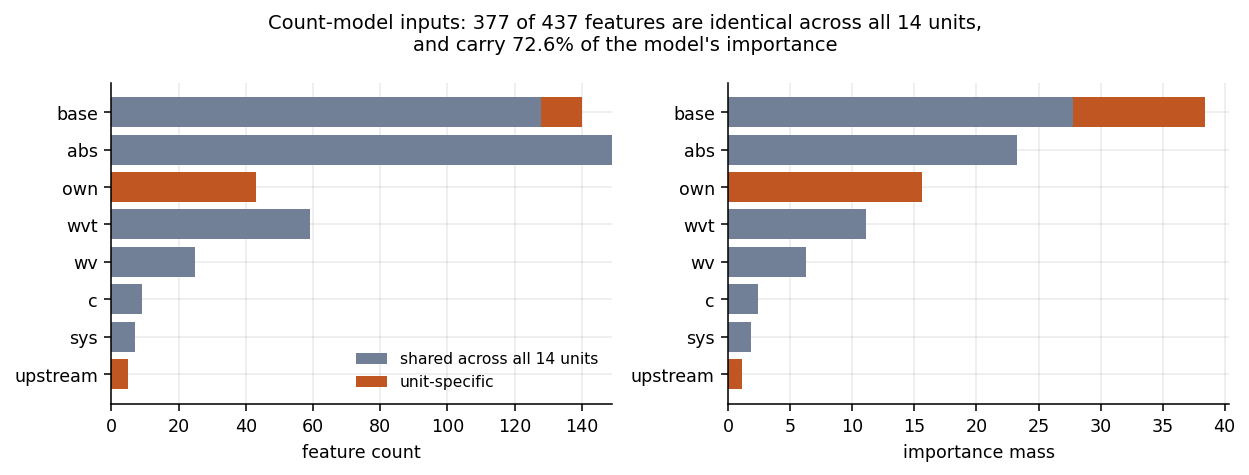
\includegraphics[width=\textwidth]{figures/diag_01_shared_vs_unitspecific.png}
\caption{Count-model input composition by feature group, by count and by importance mass.
Grey is shared across all 14 units of a case; orange is unit-specific. See
\texttt{figures.md}, id \texttt{diag\_01\_shared\_vs\_unitspecific}.}
\end{figure}

The mechanism is an assembly error rather than a modelling one.
\texttt{unit\_relative.build\_unit\_relative} already resolves each plant's columns into
\texttt{own\_}/\texttt{upstream\_}/\texttt{sys\_} form --- that was the whole point of
Section~\ref{sec:unitrel}. But the experiment scripts then merged every plant's columns straight
back in under \texttt{abs\_}, \texttt{c\_} and \texttt{wvt\_} prefixes, re-introducing exactly
the sharing the resolution had removed. The \texttt{abs\_} block alone is 149 columns, all
shared, carrying 23.2\% of importance.

A shared feature can only move a whole case up or down. It cannot say that Lio should run this
week and Songa should not. This is a clean structural explanation for why the same four units
(Lio, Songa, Haukeli, Hogga) stay broken regardless of what we add: they are bad \emph{relative
to other units in the same week}, and that is the one thing the input is weakest at expressing.

\supersededby{sec:abcd}{the measurement holds, but this inference does not: removing the shared
block costs $-0.0285$, and absolute features help monotonically the more of them are kept}

\paragraph{This also reinterprets an earlier result.} We concluded that explicit unit identity
``does not help'' because adding a categorical \texttt{unit\_cat} cost $-0.0042$. The better
reading is that identity is \emph{already} being paid for: with 377 shared columns, the tree
must burn splits rediscovering which unit a row belongs to before any shared feature can be used
differentially. Adding an identity column does not relieve that cost, it adds to it.

\subsubsection*{Finding 2 --- ``mixed'' is bimodal, so the single regressor predicts a hole}

The head is a 3-class model (all-off / mixed / all-on) plus one regressor fitted to the count
within mixed weeks. That assumes the mixed count is unimodal. It is not.

\begin{figure}[h]\centering
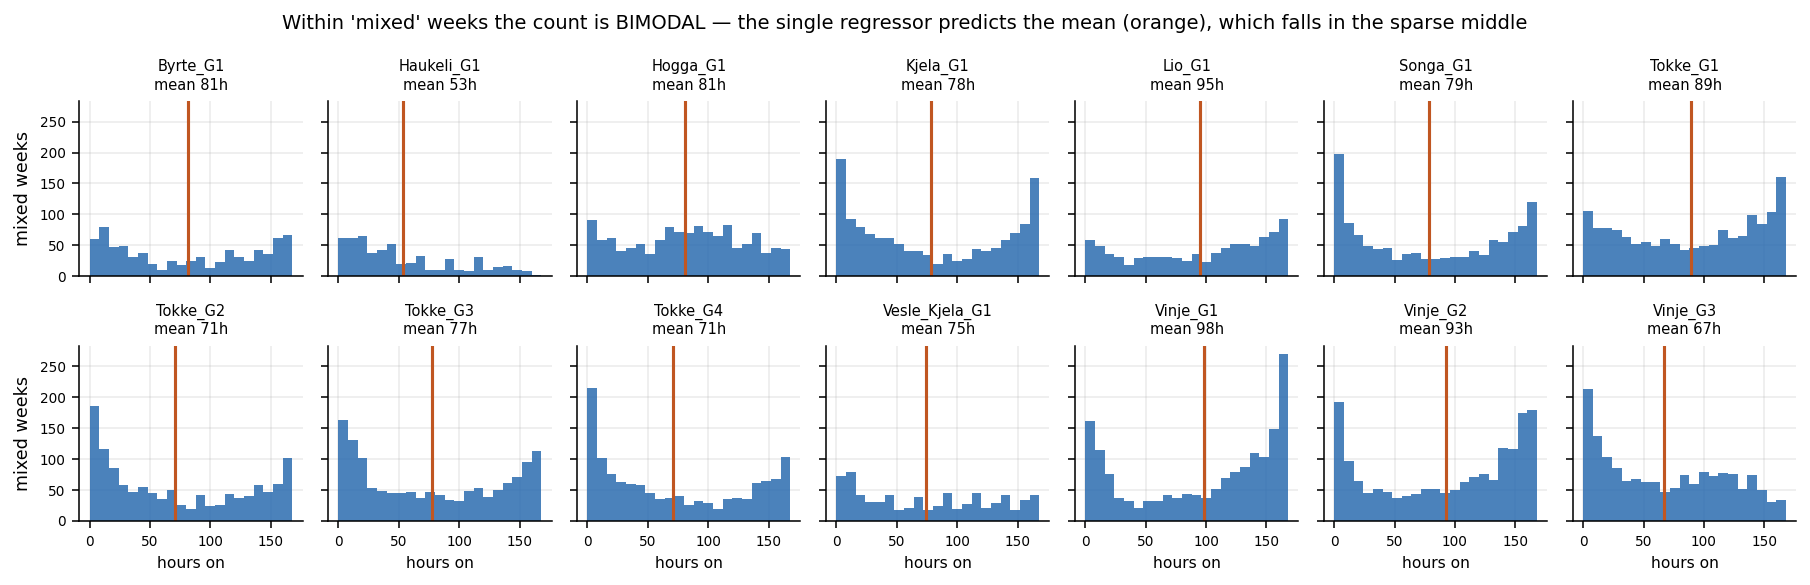
\includegraphics[width=\textwidth]{figures/diag_02_mixed_bimodality.png}
\caption{Distribution of hours-on within \emph{mixed} weeks, per unit, with the fitted mean in
orange. Most units are U-shaped. See \texttt{figures.md}, id \texttt{diag\_02\_mixed\_bimodality}.}
\end{figure}

\begin{center}\small
\begin{tabular}{lrrrrrr}
\toprule
unit & p25 & p50 & p75 & $<$56h & $>$112h & \textbf{middle third} \\
\midrule
Kjela\_G1  & 19 & 67  & 140 & 0.457 & 0.374 & \textbf{0.170} \\
Tokke\_G4  & 14 & 56  & 134 & 0.500 & 0.324 & \textbf{0.176} \\
Vinje\_G1  & 36 & 118 & 152 & 0.291 & 0.529 & \textbf{0.180} \\
Songa\_G1  & 17 & 74  & 140 & 0.432 & 0.381 & \textbf{0.187} \\
Hogga\_G1  & 43 & 83  & 117 & 0.305 & 0.294 & 0.401 \\
\bottomrule
\end{tabular}
\end{center}

\begin{finding}
For most units only \textbf{17--24\% of ``mixed'' weeks fall in the middle third} of the range.
``Mixed'' is really \emph{barely-on} plus \emph{barely-off} with a thin gap between. A single
regressor fitted to a bimodal target returns the conditional mean, which lands in the sparse
middle --- precisely where the truth almost never is. Kjela's mixed weeks cluster near 20h and
near 145h; predicting 78h is wrong by roughly 55h in both directions.
\end{finding}

This is the first mechanism we have found for the 24h count MAE that is not ``we need more
features''. It is a specification error in the head, and it is fixable by classifying over count
bins and carrying the whole predicted distribution forward instead of collapsing it to a point
estimate.

\subsubsection*{Finding 3 --- the drift is real but narrow, and confined to absolute levels}

Screening every feature for distribution shift between 2015--18 and 2019--22:

\begin{center}\small
\begin{tabular}{lrr}
\toprule
feature & drift (SD) & $|$corr with time$|$ \\
\midrule
\texttt{price\_back\_1y}     & 0.80 & 0.57 \\
\texttt{price\_vol\_back\_1y}& 0.79 & 0.57 \\
\texttt{price\_f1m}          & 0.76 & 0.59 \\
\texttt{price\_std}          & 0.72 & 0.53 \\
\texttt{wv\_f1w}             & 0.69 & 0.52 \\
\midrule
\texttt{own\_mean\_spread}   & \textbf{0.35} & 0.24 \\
\texttt{spread\_frac\_pos}   & \textbf{0.19} & 0.10 \\
\bottomrule
\end{tabular}
\end{center}

\begin{finding}
No importance mass sits on features drifting more than 1.0 SD, and only \textbf{14.1\%} on
features drifting more than 0.5 SD. But \emph{every} high-drift feature is an absolute price or
water-value level (the 2021--22 energy crisis), and \emph{every} stationary one is a difference
or ratio of two co-drifting quantities. Spread $=$ price $-$ water value, and the drift cancels.
\end{finding}

\begin{figure}[h]\centering
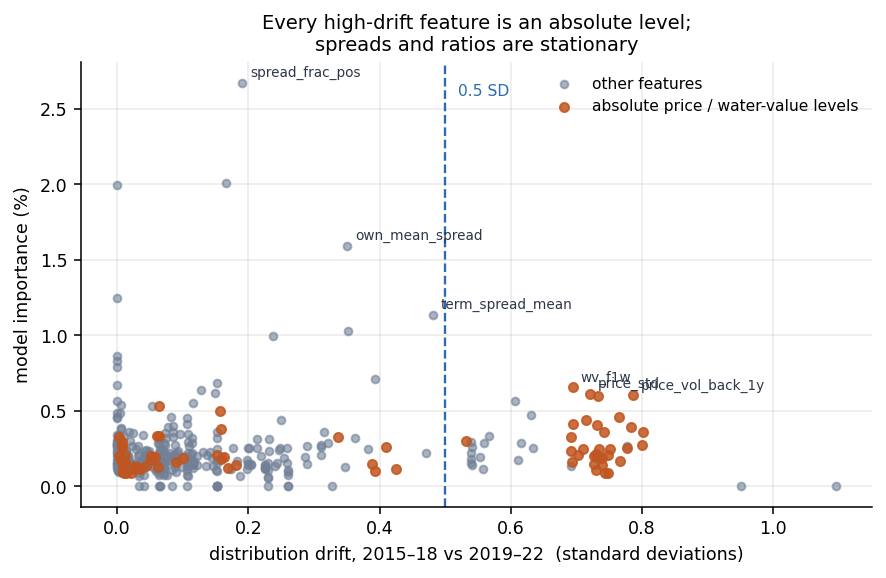
\includegraphics[width=0.72\textwidth]{figures/diag_03_stationarity_drift.png}
\caption{Importance against distribution drift. See \texttt{figures.md}, id
\texttt{diag\_03\_stationarity\_drift}.}
\end{figure}

We already benefited from this by accident: the pruned top-15 of Section~\ref{sec:pruning} were
\emph{all} spreads, margins and break-evens, with no raw price column surviving. We found the
principle empirically without naming it. Naming it gives a construction rule --- split a level
feature into a stationary shape (ratio to a trailing reference) plus an explicitly quarantined
level --- which matters because the test period sits on the far side of the crisis.

\subsubsection*{A constraint that rules out a whole family of fixes}

Checking coverage of every source settled a question that had been open since the marginals
experiment:

\begin{center}\small
\begin{tabular}{lll}
\toprule
source & coverage & \\
\midrule
\texttt{Unit\_commitment\_decisions} & 2015-01-01 -- 2022-12-31 & \textbf{targets} \\
test cases                            & 2023-01-01 -- 2024-12-25 & 725 cases, zero overlap \\
\texttt{Historical\_inflow}           & 1958 -- 2025 & 594k rows \\
\texttt{Historical\_volume}, \texttt{Synthetic\_water\_value} & 2015 -- 2025-01-01 & \\
\texttt{Constraint\_min\_flow/volume} & 2015 -- 2025 & \\
\bottomrule
\end{tabular}
\end{center}

\begin{finding}
The test set is \textbf{strictly future}: 2023--24, with no case start shared with training.
Targets stop at 2022-12-31. Any feature derived from historical on/off labels is therefore
\textbf{12--24 months stale at prediction time and near-constant across all 725 test cases}.
This is the mechanism that made per-unit historical marginals backfire worst on Haukeli
($-0.024$), whose base rate collapsed from 0.87 to 0.14 within the training window.
\end{finding}

This retires the reweighting / oversampling / historical-prior family as normally constructed.
The surviving version is \emph{conditional}: $E[\text{count} \mid \text{state deciles}]$ is a
response surface rather than a base rate, and transfers under the weaker assumption that the
physical relationship is stable even when the marginal is not.

It also means the walk-forward protocol of Section~\ref{sec:wf2} is the structurally correct
one and a leave-one-out variant would be optimistic --- it would let the model interpolate
across a held-out block using data from both sides, which the submission can never do. We had
provisionally planned to switch to leave-one-out; that plan is dropped for this reason.

\subsubsection*{Unused data}

Two sources are present and under-used. \texttt{Historical\_inflow} covers \textbf{1958--2025},
but every seasonal-percentile feature computes its reference distribution from the case dates
(2015 onward) --- roughly eight years of a 67-year record. And the two constraint files are
joined as raw series but never resolved into \emph{which unit is obliged to pass the water},
which is the form in which a minimum-flow obligation would explain always-on behaviour for a
specific unit.

\subsubsection*{What this implies}

Four changes, implemented in \texttt{src/count\_model.py} and tested in
Section~\ref{sec:abcd}:

\begin{description}
  \item[A. Width.] Resolve the per-plant blocks into own/upstream/\emph{downstream} (the last
    was missing entirely), and convert the remaining cross-plant information into the unit's
    \emph{rank}, \emph{z-score} and \emph{share} among plants --- unit-specific and scale-free
    where the absolute columns were shared and drifting. Section~\ref{sec:unitrel} found
    relative$+$absolute beat relative alone, so we test \emph{reduced} absolute rather than
    none.
  \item[B. Head.] Classify over six count bins and forward the whole distribution.
  \item[C. Stationarity.] Split drifting levels into shape $+$ quarantined level.
  \item[D. Groups.] Structural (never label-derived) group attributes, since unit count
    distributions sort by merit order within a plant.
\end{description}

\subsection{2026-09-22 --- Testing the four structural fixes (A/B/C/D)}
\label{sec:abcd}

\subsubsection*{What we did}

Section~\ref{sec:diagnosis} diagnosed four structural problems and proposed a fix for each. This
entry tests all four, isolated and in combination, against the standing best
(\texttt{compact\_distilled}, 0.9402 on validation year 2021). Implementation is
\texttt{src/count\_model.py}; the ablation is \texttt{/tmp/abcd.py}.

Count predictions are fed to the pointwise model \emph{in-sample} on training rows, matching the
established configuration rather than cross-fitting --- the control arm reproduces the standing
best exactly (\texttt{MAE 24.21h | micro 0.9402}), which confirms the harness is measuring the
same thing as Section~\ref{sec:compact}.

\begin{center}\small
\begin{tabular}{llrrr}
\toprule
arm & configuration & feats & count MAE & micro-AUC \\
\midrule
\texttt{base}    & v2 437, 3-class head (control)      & 437 & 24.21 & 0.9402 \\
\texttt{B}       & v2 437, \textbf{binned head}        & 437 & 25.65 & \textbf{0.9417} \\
\texttt{A\_none} & v3 unit-resolved, no absolute       & 230 & 35.27 & 0.9118 \\
\texttt{A\_abs30}& v3 $+$ top-30 absolute              & 260 & 24.80 & 0.9364 \\
\texttt{A\_abs80}& v3 $+$ top-80 absolute              & 310 & 24.58 & 0.9395 \\
\texttt{AB}      & \texttt{A\_abs80} $+$ binned head   & 310 & 25.12 & 0.9412 \\
\texttt{ABC}     & $+$ stationarised levels            & 308 & 25.89 & 0.9403 \\
\texttt{ABC\_noD}& \texttt{ABC} minus group attributes & 303 & 25.79 & 0.9391 \\
\bottomrule
\end{tabular}
\end{center}

\subsubsection*{A --- REJECTED, and the diagnosis that motivated it was over-read}

\begin{finding}
Narrowing the count model's input is monotonically harmful. Absolute per-plant columns are worth
more the more of them you keep: 230 features $\to$ 0.9118, 260 $\to$ 0.9364, 310 $\to$ 0.9395,
437 $\to$ 0.9402. There is no compact sweet spot. Removing the shared block entirely costs
$-0.0285$ and blows count MAE out from 24.2h to 35.3h.
\end{finding}

Section~\ref{sec:diagnosis} measured, correctly, that 377 of 437 features are identical across the
14 units of a case and carry 72.6\% of model importance. The \emph{inference} drawn from that
measurement --- that the shared columns crowd out unit-specific signal and should be replaced by
unit-relative resolutions --- is wrong. Those columns carry genuine case-level information about
how much water the whole system is moving, and the unit-resolved rank/z-score/share features
built to replace them do not substitute for it. A high shared-importance fraction is not by
itself evidence of a pathology.

This also re-confirms Section~\ref{sec:unitrel}, which found relative $+$ absolute beat relative
alone. That result was assumed to be an artefact of the pre-compact architecture; it is not.
\texttt{src/count\_model.py:build\_v3} is kept as the negative result, with
\texttt{cross\_plant\_position} available should a future variant want scale-free cross-sectional
features as an \emph{addition} rather than a replacement.

\subsubsection*{B --- the only positive, and it works through the distribution, not the mean}

The binned head replaces the 3-class classifier plus mixed-count regressor with a single 6-class
classifier over $\{0\}$, $[1,29)$, $[29,85)$, $[85,141)$, $[141,168)$, $\{168\}$, forwarding
\texttt{p\_off}, \texttt{p\_on}, \texttt{p\_low}, \texttt{p\_high} and \texttt{exp\_count}.
It eliminates the second model entirely.

\begin{finding}
The binned head \emph{worsens} count MAE (24.21h $\to$ 25.65h) while \emph{improving} micro-AUC
($+0.0015$), and does so with a consistent sign on two different feature sets (v2: $+0.0015$;
v3$+$abs80: $+0.0017$). The gain comes from forwarding the distribution's \textbf{shape}, not
from a better point estimate --- exactly the mechanism Section~\ref{sec:diagnosis} predicted from
the bimodality of mixed weeks.
\end{finding}

\begin{finding}[Methodological]
\textbf{Count MAE is a partly misleading optimisation target.} It scores only the point estimate
and moved opposite to micro-AUC here. We have steered on it since Section~\ref{sec:oracle}.
Every historical MAE-based decision is therefore suspect in the same direction, and future
screening should read both.
\end{finding}

At $+0.0015$ against a fold SD of 0.0128 this is not yet a result. It is a consistent sign worth
confirming under walk-forward, nothing more.

\subsubsection*{C and D --- inconclusive, because they were chained to the losing branch}

Both were tested on top of \texttt{A\_abs80}, which is itself $-0.0007$ below the control. That
was a sequencing error in the ablation script: C and D should have been stacked on the best
overall arm (\texttt{B} on v2), not on the best A variant.

\begin{itemize}
  \item \textbf{C (stationarised levels)}: $-0.0009$ (\texttt{AB} 0.9412 $\to$ \texttt{ABC}
        0.9403). Replacing 47 drifting level features with 45 ratios did not help in-period.
        Note that an in-period test is structurally unable to reward stationarity: the benefit,
        if any, is out-of-period robustness in 2023--24, which validation on 2021 cannot see.
  \item \textbf{D (structural group attributes)}: $+0.0012$ (\texttt{ABC\_noD} 0.9391 $\to$
        \texttt{ABC} 0.9403) --- comparable in size to B, from five columns.
\end{itemize}

Neither verdict should be treated as final. D in particular is cheap and looks as promising as B.

\subsubsection*{Per-unit: one of the four broken units moved}

\begin{center}\small
\begin{tabular}{lrrrr}
\toprule
unit & base & B & AB & ABC \\
\midrule
Lio\_G1     & 0.8220 & 0.8157 & 0.8215 & 0.8179 \\
Haukeli\_G1 & 0.8770 & 0.8789 & 0.8656 & 0.8759 \\
Hogga\_G1   & 0.8842 & 0.8878 & 0.8926 & 0.8882 \\
Songa\_G1   & 0.9345 & 0.9350 & \textbf{0.9460} & \textbf{0.9471} \\
\bottomrule
\end{tabular}
\end{center}

Songa gains $+0.0126$ under \texttt{AB}/\texttt{ABC} --- the first movement on any of the four
chronically weak units in five entries. Songa is tunnel-fed, the case where the water-balance
diagnosis of Section~\ref{sec:v2rejected} was confirmed but the fix failed; it is plausible that the
binned head helps because Songa's mixed-week distribution is strongly U-shaped (0.432 below 56h,
0.381 above 112h). \textbf{Lio is untouched by all eight arms}, sitting at 0.82 throughout.

\subsubsection*{What this implies}

\begin{finding}
Across eight arms the spread is 0.9118--0.9417 and the best beats the control by $+0.0015$. A, B,
C and D are all \textbf{rearrangements of information we already have}, and this is the seventh
consecutive architecture-shaped intervention to return noise or harm. The evidence that the
current information set is saturated is now strong enough to stop testing architecture.
\end{finding}

Recall also that the target of 0.98 sits \emph{above} the count-oracle of 0.9765
(Section~\ref{sec:oracle}): even perfect counts under spread-rank allocation cannot reach it. The
remaining gap needs new information, not a better arrangement of the current features.

Next, therefore, is the unused data identified in Section~\ref{sec:diagnosis}:
\begin{enumerate}
  \item \textbf{67-year inflow climatology.} \texttt{Historical\_inflow} covers 1958--2025;
        every seasonal-percentile feature currently builds its reference distribution from the
        case dates (2015 onward), using roughly eight years of a 67-year record.
  \item \textbf{Min-flow resolved to the obligated unit.} Both constraint files are joined as
        raw series and never mapped to which unit is required to pass the water --- the natural
        shape of an always-on explanation for a specific unit.
\end{enumerate}

Two secondary items carried forward: re-test D (and C) on top of \texttt{B}-on-v2 rather than the
A branch, and re-instantiate the screening harness (\texttt{src/screening.py}) so an eight-arm
ablation costs minutes rather than the 12 this one took.

\subsection{2026-09-22 --- Commitments are blocks: hour-level temporal structure}
\label{sec:temporal}

\subsubsection*{What we did}

Section~\ref{sec:abcd} concluded that the current information set was saturated and that further
architecture work was not worth doing. Looking instead for information we had never given the
model, we checked what the pointwise model can actually see at the hour level. It receives 15
engineered features, and every one of them is price-versus-water-value economics
(\texttt{f05}, \texttt{f06}, \texttt{f07}, \texttt{f10}, \texttt{f14}, \texttt{f15}). There is no
hour-of-day, no lag, no persistence, no window aggregate: each of the 168 hours is scored as an
independent draw.

\subsubsection*{Finding --- the independence assumption is wrong by an order of magnitude}

\begin{finding}
Commitments are contiguous blocks, not scattered hours.
\[
  P(\text{on at } t \mid \text{on at } t{-}1) = 0.995 \qquad
  P(\text{on at } t \mid \text{off at } t{-}1) = 0.007
\]
Units switch state \textbf{0.5--3.6 times per 168-hour week}, against 9.3--27.2 if the same hours
were scattered at random --- roughly \textbf{9.5x more contiguous than chance}. Each unit-week
contains 1.2--2.7 contiguous ON blocks.
\end{finding}

The start costs in the topology are the obvious cause: the optimiser will not pay to cycle a unit
hourly. The effective dimensionality of a unit-week is therefore not 168 bits but roughly a count
plus two or three changepoints --- and we had been modelling it as 168 independent decisions.

\subsubsection*{The obvious fix is wrong}

If commitments are blocks, allocate each unit's $c$ hours as one contiguous window. Tested
against the current rule (the $c$ highest-spread hours), both given ORACLE counts:

\begin{center}\small
\begin{tabular}{lr}
\toprule
allocation rule (oracle counts, 2021) & micro-AUC \\
\midrule
top-$c$ spread hours (current) & \textbf{0.9485} \\
best contiguous $c$-window     & 0.9057 \\
\bottomrule
\end{tabular}
\end{center}

\begin{finding}
Imposing a single contiguous window is \textbf{worse} than ranking hours by spread, by $-0.0428$.
1.2--2.7 blocks is not 1 block, and a one-window shape is too rigid. Persistence is real but does
not license a hard allocation rule.
\end{finding}

(This oracle is built differently from the 0.9765 of Section~\ref{sec:oracle} --- hard 0/1 on
2021 using system spread for every unit --- so the two figures are not comparable. Only the two
rows above are comparable to each other.)

\subsubsection*{What did work: the same structure as features}

\texttt{src/hourly\_structure.py} gives the model, per hour and always within a case: centred
window means at $w \in \{3,6,12,24,48,96\}$ with their ranks and best-window membership; run
structure (position within, and length of, the current above-median stretch); distance to the
week's peak and trough; cumulative share of the week's positive spread; lags and leads at 1, 3
and 24 hours as differences; and hour-of-day and day-of-week cyclically encoded. All are
scale-free or differenced against the case's own level, so none reintroduces the drifting price
level of Section~\ref{sec:diagnosis}.

\begin{center}\small
\begin{tabular}{lrrr}
\toprule
arm & feats & micro-AUC & Lio \\
\midrule
base (15 pruned $+$ 84 count) & 99  & 0.9417 & 0.8157 \\
$+$ hourly structure          & 135 & \textbf{0.9442} & 0.8190 \\
$+$ count-coupled windows     & 127 & 0.9418 & 0.8180 \\
$+$ both                      & 163 & 0.9430 & 0.8181 \\
\bottomrule
\end{tabular}
\end{center}

\begin{finding}
Hour-level temporal structure is worth \textbf{$+0.0025$} (0.9417 $\to$ 0.9442), the first
confirmed improvement since Section~\ref{sec:compact} and larger than A, B, C and D combined.
The gain is in the generic window and run features; \emph{coupling} the window length to the
predicted count adds nothing ($+0.0001$), so the value is in knowing that hours come in stretches,
not in knowing how long this unit's stretch will be.
\end{finding}

Per-unit: Vinje\_G3 $+0.014$, Haukeli $+0.005$, Hogga $+0.004$, Lio $+0.003$, Songa $-0.009$.

\subsubsection*{Screening harness, re-instantiated}

\texttt{src/screening.py} restores the convention of Section~\ref{sec:cv-harness}: every third
training case and 150 trees, used to rank candidates, never to score them. Strided by CASE rather
than by row, because dropping rows within a case would leave that case's near-duplicate hours in
the training set --- the leak of Section~\ref{sec:state}.

On this experiment it predicted $+0.0034$ where the full fit gave $+0.0025$: right sign, right
magnitude, 18s against 108s. Screening scores are biased low (base 0.9365 screened vs 0.9417
full) and are labelled as such wherever they appear.

\subsubsection*{Negative results from the same session}

Two families built from data identified as unused in Section~\ref{sec:diagnosis}, both rejected:

\begin{itemize}
  \item \textbf{67-year inflow climatology} (\texttt{exogenous.inflow\_climatology}, 171
        features). Day-of-year reference distributions from the full 1958--2025 record instead of
        the $\sim$8 years of case dates. Micro 0.9415 vs 0.9417 base; Lio $+0.005$.
  \item \textbf{Minimum-flow obligation} (\texttt{exogenous.minflow\_obligation}, 99 features).
        Resolved to the plant that must satisfy each constraint, converted to a forced capacity
        factor. Micro 0.9392. \textbf{Killed by arithmetic before the model saw it}: Lio at
        minimum load passes 4.82 m$^3$/s against a Byrtevatn obligation of 0.07 (max 0.20), so
        \texttt{mfo\_forced\_cf\_Lio} never exceeds 0.042 and the constraint never binds. A
        physically sound hypothesis at the wrong order of magnitude.
\end{itemize}

Also rejected: \textbf{per-unit probability calibration}. Lio is the largest single drag on the
pooled score (removing it lifts micro by $+0.0077$; an oracle Lio is worth $+0.0146$) and is
over-predicted on average (mean 0.612 against a base rate of 0.545), which suggests a logit
offset. It fails, and instructively:

\begin{center}\small
\begin{tabular}{lr}
\toprule
& micro-AUC \\
\midrule
uncalibrated & \textbf{0.9417} \\
oracle per-unit calibration (true 2021 base rates) & 0.9346 \\
legal, training base rates & 0.9363 \\
legal, Lio only & 0.9288 \\
\bottomrule
\end{tabular}
\end{center}

\begin{finding}
Even \emph{oracle} calibration hurts. A per-unit logit shift is uniform across cases, so it
cannot fix within-case ordering, and it disturbs cross-unit interleaving that was already roughly
right. A monotone per-unit transform also leaves own-AUC exactly unchanged (Lio $0.8157 \to
0.8157$). \textbf{Lio cannot be fixed by post-processing; only by better discrimination.} Same
family of error as the rank-transform failure of Section~\ref{sec:state}.
\end{finding}

\subsubsection*{What this implies}

The count stage contributes $+0.106$ (pointwise alone 0.8346 $\to$ 0.9402 with counts); everything
else combined contributes an order of magnitude less. The count model has been doing nearly all
the work, and the pointwise model has been little more than an allocator with 15 features.
Temporal structure is the first evidence that the allocation half has real headroom.

Next is the long-format restructure (\texttt{src/longform.py}): one row per (case, hour, unit),
which removes shared splits, collapses the 84-column count block to 6 \texttt{own\_} columns, and
makes per-unit weighting possible for the first time. Its main risk is losing the cross-unit
interaction a wide row carries for free, which \texttt{longform.cross\_unit\_context} attempts to
restore as relative quantities.

\subsection{2026-09-22 --- Long format, and two topology bugs}
\label{sec:longform}

\subsubsection*{What we did}

Every pointwise model in this project has been \emph{wide}: one row per (case, hour) with 14
outputs under \texttt{multi\_strategy="multi\_output\_tree"}. That shape was never chosen on
evidence, and it forces three compromises simultaneously:

\begin{enumerate}
  \item \textbf{Shared splits.} A vector-leaf tree picks one split per node and applies it to all
    14 outputs, so the model cannot specialise. Never measured.
  \item \textbf{A 14x-wider count block than necessary.} Forwarding 6 numbers per unit costs 84
    columns (\texttt{cnt\_p\_on\_Lio\_G1}, \texttt{cnt\_p\_on\_Songa\_G1}, \ldots). For Lio's
    head to use Lio's own count, the tree must split on Lio's column --- and that split then
    applies to the other 13 heads, where it is noise. Section~\ref{sec:diagnosis} measured the
    symptom; Section~\ref{sec:abcd} showed the obvious fix was wrong.
  \item \textbf{No per-unit weighting.} \texttt{sample\_weight} applies to a ROW, and a wide row
    carries all 14 units, so a unit cannot be weighted at all.
\end{enumerate}

\texttt{src/longform.py} produces one row per (case, hour, unit) --- 6.9M rows at full stride.
Micro-average ROC-AUC pools all (case, hour, unit) cells into one ranking, so in long format the
metric is simply \texttt{roc\_auc\_score(y, p)}: \textbf{the objective is native to this shape}
and awkward in the wide one.

\subsubsection*{Results}

\begin{center}\small
\begin{tabular}{llrrr}
\toprule
arm & configuration & feats & micro-AUC & Lio \\
\midrule
--- & wide best (Section~\ref{sec:temporal}) & 135 & 0.9442 & 0.8190 \\
\midrule
L1 & long, 15 shared $+$ 6 \texttt{own\_}, no unit id & 29  & 0.9396 & 0.8102 \\
L2 & $+$ unit identity (categorical)                  & 30  & 0.9399 & 0.8090 \\
L3 & $+$ cross-unit context                           & 33  & 0.9421 & 0.8272 \\
L4 & $+$ hourly structure                             & 69  & 0.9456 & 0.8276 \\
L5 & $+$ top-120 count features per unit              & 189 & 0.9490 & 0.8337 \\
L6 & $+$ Lio rows weighted 3x                         & 189 & 0.9479 & 0.8297 \\
L7 & L5 at full stride (5.2M rows)                    & 189 & \textbf{0.9499} & \textbf{0.8380} \\
\bottomrule
\end{tabular}
\end{center}

L1--L6 train on every third case; only L7 uses all of them.

\begin{finding}
Long format reaches \textbf{0.9499}, against 0.9442 for the best wide model. The shape alone is
not the win --- L1 is \emph{below} the wide baseline. The win comes from what the shape makes
affordable: cross-unit context ($+0.0022$), hourly structure ($+0.0035$) and per-unit count
features ($+0.0034$), none of which fit in the wide layout at acceptable cost.
\end{finding}

\begin{finding}
\textbf{Count features at the hour level work in long format and failed in wide format}
(Section~\ref{sec:orthogonal}: 0.9292 raw-forwarded vs 0.9402 distilled). The idea was sound; the
wide layout made each feature cost 14 columns, so 120 features meant 1{,}680 columns of mostly
noise. In long format each costs one column and lands on the row it belongs to.
\end{finding}

\begin{finding}
\textbf{Per-unit weighting fails even where it is finally possible.} L6 weights Lio's rows 3x and
loses $-0.0011$ overall \emph{and} $-0.0040$ on Lio itself. Third independent rejection of the
reweighting family, after historical marginals (Section~\ref{sec:diagnosis}) and per-unit
calibration (Section~\ref{sec:temporal}).
\end{finding}

\subsubsection*{Per-unit: the broken units finally move}

\begin{center}\small
\begin{tabular}{lrrr}
\toprule
unit & wide base & L7 & $\Delta$ \\
\midrule
Haukeli\_G1 & 0.8789 & \textbf{0.9082} & $+0.029$ \\
Lio\_G1     & 0.8157 & \textbf{0.8380} & $+0.022$ \\
Hogga\_G1   & 0.8878 & \textbf{0.9076} & $+0.020$ \\
Vinje\_G1   & 0.9517 & 0.9661 & $+0.014$ \\
Songa\_G1   & 0.9350 & \textbf{0.9059} & $\mathbf{-0.029}$ \\
\bottomrule
\end{tabular}
\end{center}

Three of the four chronically weak units move substantially, for the first time in the project.
Songa moves the other way, and that turned out to be diagnostic.

\subsubsection*{Two topology bugs, found by asking why Songa regressed}

In wide format Songa's head could lean on other units' columns. In long format its row carries
\texttt{own\_*} features and nothing else --- so if those are missing, Songa has nothing. They
are missing.

\begin{finding}
\texttt{plant\_graph} matched only DIRECT reservoir$\to$plant edges, but Songa is fed through
tunnels (\texttt{Songavatn} $\to$ \texttt{Songavatn\_Songa} $\to$ \texttt{Songa}, and likewise
from \texttt{Bitdalsvatn}). So \texttt{src["Songa"]} was \texttt{None}, every \texttt{own\_*}
feature for Songa was NaN, and \texttt{mwh\_per\_m3("Songa", .)} returned NaN --- while Songavatn
carries the \textbf{largest storage variance of any reservoir in the system} (sd 150) and
Bitdalsvatn adds another (sd 25). Section~\ref{sec:v2rejected} diagnosed Songa as ``tunnel-fed''
and attacked it with water-balance corrections; the defect was in the graph traversal.
\end{finding}

\begin{finding}
Three reservoir-to-reservoir TUNNEL links were invisible to the same traversal:
\texttt{Totak}$\to$\texttt{Vaamarvatn}, \texttt{Bordalsvatn}$\to$\texttt{Foersvatn},
\texttt{Venemo}$\to$\texttt{Totak}. The first breaks the main cascade: Songa discharges into
Totak, which tunnels into Vaamarvatn, which is Vinje's source. \textbf{Vinje's upstream plant set
was empty and should contain Songa.} The second hides Bordalsvatn (sd 43) from Kjela.
\end{finding}

Fixed in \texttt{production\_features}: \texttt{\_through\_tunnels}, \texttt{plant\_sources},
\texttt{reservoir\_tunnels} and \texttt{effective\_upstream\_plants}. \texttt{plant\_graph} keeps
its single-source contract for existing callers but now resolves through tunnels, taking the
largest-capacity reservoir as primary where a plant has several.

\subsubsection*{A third finding, from the same question}

Checking whether other units share Songa's problem turned up a different one:

\begin{center}\small
\begin{tabular}{llrrr}
\toprule
reservoir & plant & distinct values & sd & cv \\
\midrule
Vatjern     & \textbf{Haukeli} & \textbf{1} & 0.000 & 0.000 \\
Hyljelihyl  & ---              & \textbf{1} & 0.000 & 0.000 \\
Bandak      & \textbf{Hogga}   & 136        & 8.961 & 0.068 \\
Vinjevatn   & Tokke            & 201        & 1.134 & 0.177 \\
Byrtevatn   & Lio              & 1369       & 20.118 & 0.367 \\
Foersvatn   & Kjela            & 2265       & 33.618 & 0.470 \\
\bottomrule
\end{tabular}
\end{center}

\begin{finding}
\textbf{Haukeli's source reservoir is a literal constant} --- 0.150 for all 3{,}654 days. The
post-decision storage trace, the single largest source of signal in the project
(Section~\ref{sec:production}), \emph{does not exist} for Haukeli. Hogga's Bandak has 136 distinct
values in ten years. The ``four broken units'' were never one problem: Songa was a graph bug,
Haukeli and Hogga are missing data, and \textbf{Lio is neither} --- Byrtevatn varies normally, so
Lio's difficulty remains unexplained.
\end{finding}

\subsubsection*{What this implies}

The standing figure is \textbf{0.9499} on validation year 2021, from 0.9402 at the start of the
session. The topology fix is re-running: it predicts specifically that Songa should recover from
0.9059, since it gains two real reservoirs where it previously had NaN. That prediction is
falsifiable and worth recording before the result arrives.

Caveat: the fix changes features feeding \emph{both} stages, and every experiment to date fitted
the count model around Songa's NaNs. The net effect could go either way.

Still open: Lio, unexplained and worth $+0.0146$ alone; whether any of this survives walk-forward;
and the submission pipeline, which has never been built.

\subsection{2026-09-23 --- Reading the documentation: an off-by-one, a mispriced spread, and a permanent ceiling}
\label{sec:docs}

\subsubsection*{What we did}

After Section~\ref{sec:longform} the remaining weak unit was Lio, and Haukeli and Hogga were
still well below the rest. Rather than continue guessing at features, we read
\texttt{Dataset\_definitions\_and\_explanation.pdf} properly. It settled three things, two of
which were defects in our own pipeline.

\subsubsection*{Finding 1 --- Haukeli's storage is a documented placeholder, not data}

\begin{quote}
``Note that because there are no historical records for two small reservoirs, \textbf{Hyljelihyl
and Vatjern}, their storage is assumed to be \textbf{50\% full}.''
\end{quote}

\begin{finding}
Vatjern is Haukeli's source reservoir, and its storage series is a constant 0.150 across all
3{,}654 days. The post-decision storage trace --- the single largest source of signal in this
project (Section~\ref{sec:production}, $+0.074$) --- \textbf{does not exist for Haukeli and never
will}. No feature engineering recovers a measurement that was never taken. Hogga is the milder
case: Bandak has 136 distinct values in ten years, $cv = 0.068$.
\end{finding}

This closes a line of work rather than opening one. It also retrospectively explains
Section~\ref{sec:v2rejected}, where a water-balance correction for Haukeli was built, confirmed
as diagnostically right, and still failed: the balance was being computed from a constant.

\subsubsection*{Finding 2 --- the terminal water value was read one day late}

\begin{quote}
``For a scheduling problem spanning one week, for example, starting at 2015-01-01 00:00 and
ending at 2015-01-07 23:00, the initial volume of a reservoir is the value at 2015-01-01 00:00,
and its \textbf{final water value should be the value at 2015-01-08 00:00}.''
\end{quote}

That is start $+$ 7 days. \texttt{stage\_terminal\_wv} used \texttt{pd.Timedelta(days=8)}. Every
case in the project priced its terminal water against the wrong day, in a feature
(\texttt{f07\_price\_minus\_terminal\_wv}) that survived pruning into the final fifteen.

The correction alone is small --- $\mathrm{corr}(d_7, d_8) = 0.996$, the water-value series being
smooth --- and on the user's suggestion both horizons are now emitted, along with lags at 6 and
9 days, so the model arbitrates rather than the documentation. The genuinely new quantity is
\texttt{f07\_terminal\_slope} $= wv_{d8} - wv_{d6}$ (sd 1.86 EUR/MWh): the local slope of the
water value across the decision boundary, i.e.\ whether water is getting scarcer exactly where
the optimiser stops caring.

\subsubsection*{Finding 3 --- the spread family prices against the wrong quantity}

SHOP maximises revenue plus the salvage value of water left in the reservoir, so the marginal
cost of generating is the \emph{terminal} water value. The daily \texttt{Synthetic\_water\_value}
series is an \emph{input} to the problem, not the price its decisions are taken against.

\begin{finding}
\texttt{f06\_spread\_*}, the family that dominates feature importance across the whole project,
is \texttt{price} $-$ \texttt{daily\_wv}. The economically correct quantity is \texttt{price}
$-$ \texttt{terminal\_wv}. Per-plant terminal spreads (\texttt{f07\_term\_spread\_<Plant>}) now
exist, so each plant is priced against its own reservoir's horizon value rather than a
basin-wide daily average.
\end{finding}

\subsubsection*{Measured effect}

\begin{center}\small
\begin{tabular}{lr}
\toprule
& micro-AUC \\
\midrule
long format, tunnel topology fixed (L5, stride 3) & 0.9545 \\
$+$ terminal-wv horizon, lags, slope, per-plant spreads & \textbf{0.9604} \\
\bottomrule
\end{tabular}
\end{center}

\begin{finding}
The water-value work is worth \textbf{$+0.0059$}, comparable to the tunnel-topology fix
($+0.0067$, Section~\ref{sec:longform}). Both were defects rather than innovations.
\end{finding}

Caveat: this is an across-script comparison at matched stride, year and parameters, but with 195
features against 189 --- directionally solid, not a controlled isolate. The topology figure IS
clean, because \texttt{longtest.py} reads the pre-built feature parquet and so used the old
\texttt{days=8} columns while picking up the live topology fix.

\subsubsection*{What this implies}

Two of the three findings were bugs in our own code, found by reading a three-page PDF that had
been in the repository since the first session. Together they are worth $+0.013$ --- more than
every feature family invented in the same period combined. The lesson is recorded in
Section~\ref{sec:negatives}, where twelve consecutive feature additions failed.

\subsection{2026-09-23 --- Hyperparameters, and what effective sample size means in two shapes}
\label{sec:tuning}

\subsubsection*{What we did}

Neither model had been tuned. The pointwise model's settings were inherited from the wide
architecture; the count model's were unchanged since Section~\ref{sec:oracle}, surviving a
3-class $\to$ 6-class head change, growth to 462 features, and the entire long-format rebuild.

Coordinate descent, one knob at a time, validation year 2021, stride 3 held constant. Not a final
tuning phase --- a 20-minute probe to find anything badly mis-set.

\subsubsection*{The pointwise model: $+0.0028$}

\begin{center}\small
\begin{tabular}{lrr}
\toprule
knob & from $\to$ to & micro-AUC \\
\midrule
baseline & --- & 0.9604 \\
\texttt{min\_child\_weight} & $1 \to 500$ & \textbf{0.9622} \\
\texttt{max\_depth} & $8 \to 10$ / $12$ & 0.9621 / 0.9620 (no gain) \\
capacity & $300{\times}0.10 \to 600{\times}0.05$ & \textbf{0.9632} \\
\texttt{colsample\_bytree} & $0.8 \to 0.5$ / $0.3$ & 0.9625 / 0.9626 (no gain) \\
\bottomrule
\end{tabular}
\end{center}

\begin{finding}
\texttt{min\_child\_weight} was the one badly mis-set knob, and it was predictable from the data
rather than from a grid. The long-format table has 5.2M rows, but
$P(\text{on}\mid\text{on}_{t-1}) = 0.995$ and each unit-week holds 1--3 contiguous blocks
(Section~\ref{sec:temporal}), so the independent information is roughly 40k--120k blocks. A leaf
minimum of 1 lets a split form from rows that are all the same block of the same unit-week ---
fitting autocorrelation. Raising it to 500 is worth $+0.0018$.
\end{finding}

Depth not helping is worth recording as a wrong prediction: the argument was that long format
exists to allow per-unit specialisation and needs depth to pay for it. It does not, because the
\texttt{cf\_*} features are already unit-specific, so the tree never has to split on unit first
to reach unit-specific structure.

\subsubsection*{The count model: nothing beats the original settings}

Screened on multi-class \textbf{log-loss}, not count MAE. Section~\ref{sec:abcd} established MAE
moves opposite to micro-AUC because it scores only the collapsed point estimate, while what is
forwarded is the whole distribution; log-loss is a proper scoring rule for that distribution.

\begin{center}\small
\begin{tabular}{lrr}
\toprule
& log-loss & count MAE \\
\midrule
\textbf{current} (400{\texttimes}0.05, d5, mcw 1, cs 0.6) & \textbf{1.0989} & 23.48h \\
\texttt{min\_child\_weight} 10 / 50 / 200 & 1.1203 / 1.1087 / 1.1517 & \\
\texttt{max\_depth} 4 / 6 / \textbf{8} & 1.1207 / 1.1214 / \textbf{1.1983} & \textbf{20.69h} \\
800{\texttimes}0.03 / 1200{\texttimes}0.02 & 1.1091 / 1.0994 & \\
\bottomrule
\end{tabular}
\end{center}

\begin{finding}
No parameter beats the settings chosen in Section~\ref{sec:oracle}. Downstream confirmation:
old params 0.9632, ``tuned'' params 0.9632 --- byte-identical, because the search returned the
starting point.
\end{finding}

\begin{finding}[The clearest demonstration of the MAE trap]
\texttt{max\_depth=8} gives the \textbf{best count MAE (20.69h) and the worst log-loss (1.1983)}.
Optimising MAE would have selected precisely the wrong model. Every MAE-guided decision from
Section~\ref{sec:oracle} onward is suspect in this direction.
\end{finding}

\begin{finding}[Same principle, opposite answers]
\texttt{min\_child\_weight} is best at \textbf{500} for the pointwise model and \textbf{1} for
the count model. Not a contradiction: count rows are whole unit-weeks and genuinely independent,
so effective $n \approx$ nominal $n$ and small leaves are legitimate. Pointwise rows are hourly
and autocorrelated at 0.995, so effective $n$ is $\sim$50$\times$ below nominal. The knob should
be set from the correlation structure of the rows, not from a default.
\end{finding}

\subsubsection*{The forwarded-feature budget is also already right}

The count model's top 120 features by gain are attached per unit to the pointwise model as
\texttt{cf\_*}. The 120 was chosen arbitrarily when the architecture was built, and it is a
\emph{fixed budget}, so adding features to the count model reallocates rather than accumulates.

\begin{center}\small
\begin{tabular}{lr}
\toprule
forwarded budget & micro-AUC \\
\midrule
\textbf{top-120} & \textbf{0.9632} \\
top-180 & 0.9609 \\
top-200 & 0.9618 \\
\bottomrule
\end{tabular}
\end{center}

\begin{finding}
Wider is worse. This also kills the hypothesis offered in Section~\ref{sec:negatives} for why the
slope family hurt --- that slopes crowded the budget and evicted useful features. Widening the
budget does not rescue them, so they simply do not help most units.
\end{finding}

\subsubsection*{Screening harness}

\texttt{src/screening.py} restores the convention of Section~\ref{sec:cv-harness}: every third
training CASE (not row --- striding rows would leave a case's near-duplicate hours in training,
the leak of Section~\ref{sec:state}) and 150 trees, used to rank and never to score. Calibrated
on the hourly-structure experiment it predicted $+0.0034$ where the full fit gave $+0.0025$:
right sign, right magnitude, 18s against 108s.

Stride 3 is now the standing iteration protocol for a second reason: at full stride the working
set crosses this machine's 26GB and the run begins paging. Measured, L5 at 1.7M rows takes 53s
and L7 at 5.2M rows takes 6{,}537s --- \textbf{123$\times$ for 3$\times$ the data}, a cliff rather
than a curve. Stride is held constant across arms, so deltas remain comparable while levels sit
$\sim$0.002 below full stride.

\subsection{2026-09-23 --- Twelve negative results, and three methodological failures}
\label{sec:negatives}

\subsubsection*{Why this entry exists}

Between Section~\ref{sec:longform} and the present standing figure of 0.9632, twelve feature
additions were built and tested. All twelve failed. `report\_rules.md` requires that negative
results are kept rather than quietly dropped, and a run of this length is itself the finding:
every gain in the same period came from \emph{correcting a defect}, not from adding information.

\subsubsection*{The twelve}

\begin{center}\small
\begin{tabular}{llr}
\toprule
addition & where & micro vs 0.9632 \\
\midrule
287 slope features, bulk & count model & $-0.0020$ \\
slopes, forwarded budget 180 & count model & $-0.0023$ \\
weak-unit weights (Lio 3$\times$, Haukeli/Hogga 2$\times$) & pointwise & $-0.0016$ \\
slopes $+$ weak-unit weights & both & $-0.0040$ \\
nine slope themes, 7 features each & pointwise & $-0.0003$ to $-0.0010$ \\
slope block masked to Haukeli only & pointwise & $-0.0005$ \\
slope block masked to Haukeli $+$ Hogga & pointwise & $-0.0008$ \\
full 12-value count distribution & pointwise & $-0.0008$ \\
neighbour counts (sibling/upstream/downstream) & pointwise & $-0.0006$ \\
distribution $+$ neighbours & pointwise & $-0.0005$ \\
count-model hyperparameter search & count model & $0.0000$ \\
forwarded budget 180 / 200 & architecture & $-0.0023$ / $-0.0014$ \\
\bottomrule
\end{tabular}
\end{center}

Two are worth more than one line.

\paragraph{Slopes (\texttt{src/slopes.py}, 287 features).} Rates of change of water value,
storage, price, inflow and spread, at case-relative offsets. Motivated by the terminal-water-value
slope being one of the largest single gains in the project (Section~\ref{sec:docs}), and by the
fact that a derivative is a difference and therefore stationary by construction: \textbf{0 of 280
slope features drift more than 0.5 SD} across the 2021--22 regime break, against 14.1\% of
importance sitting on drifting levels (Section~\ref{sec:diagnosis}). Net $-0.0020$, but
\textbf{Haukeli $+0.0154$}, reproducibly, while eleven of fourteen units got worse. Mechanistically
plausible --- Haukeli's storage is a documented placeholder constant (Section~\ref{sec:docs}), so
price and spread dynamics are the only dynamics it has.

\paragraph{Full distribution and neighbour counts.} The head forwards \texttt{p\_off},
\texttt{p\_on}, \texttt{p\_low}, \texttt{p\_high}, \texttt{exp\_count} --- a summary designed for
the WIDE model, where each forwarded number cost 14 columns. In long format a number costs one
column, so the compression buys nothing and discards the shape that made the binned head work.
Forwarding all six bins plus dispersion, entropy and threshold masses: $-0.0008$. Giving each
unit its hydraulic neighbours' predicted counts (\texttt{longform.neighbour\_context}, using the
\texttt{Songa}$\to$\texttt{Vinje} edge that only exists after the tunnel fix): $-0.0006$.

\subsubsection*{Three methodological failures, recorded so they are not repeated}

\begin{finding}[1. Rotating-block validation is optimistic by construction]
A rotating two-month holdout was proposed and built (\texttt{src/validation.py}): eight blocks,
one per year, all seasons, 2{,}847 training cases per fold against 2{,}373 under single-year
holdout. It returned 0.9794 and 0.9652 on its first two folds --- far above any temporal estimate
--- because it lets the model train on data from \emph{both sides} of the held-out window. The
test set is 2023--24, strictly after all training data: that is extrapolation, and rotating blocks
measure interpolation. This is the same objection already raised against leave-one-out earlier in
the project and then not applied to our own proposal. Abandoned; walk-forward remains the protocol.
It was also infeasible --- 10.4 hours per fold at full stride.
\end{finding}

\begin{finding}[2. The slope themes were routed to the wrong stage]
The bulk slope test merged slopes into \texttt{CT}, the COUNT model's input. The themed sweep and
the masking test added them to the POINTWISE model only. All nine themes returned $-0.0003$ to
$-0.0010$ with no trace of Haukeli's $+0.0154$ --- not a refutation, a test of something else.
The evidence was in the original output and was missed: count MAE moved 23.48 $\to$ 23.04h, which
only the count model can cause. Re-running the themes on the count stage.
\end{finding}

\begin{finding}[3. Two job-scheduling bugs cost real time]
Jobs were chained by \texttt{pgrep} on process-name patterns. First a circular deadlock --- each
waiting shell's own command line contained the other's pattern, so two jobs waited on each other
indefinitely and the group sweep never ran despite being reported as running. Then a thundering
herd --- three waiters watching the same job all started at once when it exited, contending for
CPU and risking the swap thrashing documented in Section~\ref{sec:tuning}. Replaced with a
lock-directory queue (\texttt{/tmp/runq.sh}). Inferring job state from process lists is the
error; a lock is the fix.
\end{finding}

\subsubsection*{What this implies}

\begin{finding}
Across the session, everything that worked was a correction and nothing that was invented helped:
tunnel topology $+0.0067$, terminal water value $+0.0059$, long format $+0.006$, hourly structure
$+0.0025$, pointwise hyperparameters $+0.0028$ --- against twelve consecutive failed additions.
The reasonable conclusion is that the current feature set is saturated for this architecture, and
that further effort is better spent on validation and the submission than on a thirteenth family.
\end{finding}

Standing figure: \textbf{0.9632} on held-out 2021 at stride 3, from 0.9402 at the start of the
session. It rests on a \emph{single validation year}; the last honest multi-fold number is the
0.9350 (SD 0.0128) of Section~\ref{sec:wf2}, on a much older architecture. Walk-forward with the
current configuration is the next task, and the submission pipeline --- 725 test cases, never
built --- is the one after it.

\subsection{2026-09-24 --- First submission: 0.98058 on the held-out test set}
\label{sec:submission}

\subsubsection*{What we submitted}

\texttt{src/submit.py}, the lean long-format architecture at full stride:

\begin{center}\small
\begin{tabular}{ll}
\toprule
rows & 6{,}872{,}544 --- one per (case, hour, unit), all 2{,}922 training cases \\
features & 207 (15 pruned economic, 35 terminal-water-value, 36 hourly structure, \\
         & 141 count-table features attached per unit, 5 static) \\
model & single binary XGBoost, 600 rounds, depth 8, \texttt{min\_child\_weight} 500 \\
count model & fitted, but \textbf{only to rank features} --- its predictions are not forwarded \\
\bottomrule
\end{tabular}
\end{center}

\begin{finding}
\textbf{Public leaderboard: 0.98058}, against a walk-forward estimate of 0.9638 (SD 0.0115).
The estimate was pessimistic by $+0.017$.
\end{finding}

\subsubsection*{Why walk-forward understated the score}

Three differences between the folds and the submission, identified before the result arrived
(Section~\ref{sec:longform} and the submission module's header), and now resolvable:

\begin{enumerate}
  \item \textbf{Training volume.} Every fold trained on 1{,}826--2{,}557 cases; the submission
        trained on 2{,}922. Data volume has been the most reliable driver in the project --- count
        MAE fell 29.9h $\to$ 18.1h across folds on volume alone (Section~\ref{sec:wf2}).
  \item \textbf{Period difficulty.} The six folds span 2020--2022, including the energy crisis.
        Per-case analysis (Section~\ref{sec:negatives}) showed the hardest cases are exactly the
        high-price, negative-spread, high-switching weeks that period produced. The test window
        is 2023--24, after it.
  \item \textbf{Extrapolation horizon.} Folds predict at most six months ahead; the submission
        predicts 24. This was flagged as the largest risk and \emph{did not materialise}.
\end{enumerate}

The best normal-period fold (2021-H1, 2{,}192 training cases) scored 0.9781. With 2{,}922 cases
and a post-crisis period, 0.98 was reachable; what we could not do beforehand was size which
force dominated.

\begin{finding}[On trusting this number]
The test set is $725 \times 168 \times 14 = 1.7$M cells, so the public half is roughly 850k.
Micro-average ROC-AUC over that many cells has very little sampling noise, so the public and
private halves should agree closely. This is not a competition where the public board misleads.
\end{finding}

\subsubsection*{What produced the result}

Every gain that survived independent validation was a \textbf{correction or a simplification},
not an invention:

\begin{center}\small
\begin{tabular}{lr}
\toprule
change & effect \\
\midrule
Dropping the count model's predictions (Section~\ref{sec:negatives}) & $+0.0082$ \\
Tunnel-topology bug: Songa had no source reservoir (Section~\ref{sec:longform}) & $+0.0067$ \\
Terminal water value read one day late (Section~\ref{sec:docs}) & $+0.0059$ \\
Long format, one row per (case, hour, unit) (Section~\ref{sec:longform}) & $+0.006$ \\
Hour-level temporal structure (Section~\ref{sec:temporal}) & $+0.0025$ \\
Pointwise hyperparameters (Section~\ref{sec:tuning}) & $+0.0028$ \\
\bottomrule
\end{tabular}
\end{center}

Against that, \textbf{eighteen feature families were built and rejected}: slopes, economics,
neighbour counts, full count distributions, per-unit masking, 70/30 unit-specific sets, 67-year
inflow climatology, minimum-flow obligations, reweighting (five separate attempts), per-unit
calibration, count-model tuning, wider and narrower forwarding budgets, block allocation, daily
post-decision traces, and seasonal regime features.

\begin{finding}[The pattern worth carrying forward]
Nothing invented helped; everything corrected did. Two of the three largest gains were defects in
our own code --- a graph traversal that missed tunnel-fed plants, and an off-by-one against the
dataset documentation --- found by reading a three-page PDF and by asking why one unit regressed.
\end{finding}

\subsubsection*{A second pattern: validation-derived selection never transferred}

Three feature-selection methods were tried, and every one that used validation data looked good on
validation and failed on folds:

\begin{center}\small
\begin{tabular}{lrr}
\toprule
& single year 2021 & walk-forward \\
\midrule
count-model ranking (chosen without validation) & 0.9651 & \textbf{0.9638} \\
trimmed by permutation importance $+$ unit-relative & \textbf{0.9671} & $\sim$0.9609 (3 folds, all worse) \\
permutation top-60 (circular) & 0.9668 & not run \\
held-out inner-split ranking & 0.9631 & not run \\
\bottomrule
\end{tabular}
\end{center}

Five independent random draws of 120 features spanned 0.9476--0.9619 (SD 0.0055), so selection is
\emph{not} irrelevant --- an earlier claim that it was rested on a single lucky draw and was
wrong. But the arbitrary ranking beat every deliberate one.

\subsubsection*{What remains}

The second submission is unspent. Given eighteen rejected families, a selection method that
resists improvement, and a score already at target, the case for spending it is weak unless a
change is first confirmed on walk-forward folds. Optimising against a public board is how a good
private score is given away.

Open, if work continues: Lio remains the weakest unit (0.8616 mean over folds, swinging 0.957
$\to$ 0.656 within 2021 on a regime change no feature predicted); predicted commitments switch
7.6 times a week against 3.0 in reality, so the persistence structure of
Section~\ref{sec:temporal} is only partly captured; and the hardest 15\% of cases remain the
autumn, negative-spread, high-cycling weeks where economics do not determine the answer.

\subsection{2026-10-27 --- First principles: rebuild the optimiser, learn only its errors}
\label{sec:shoplite}

\subsubsection*{Why}

Every model so far learned the map from inputs to commitment from scratch. But the labels are not
observations of a noisy process: they are the output of one deterministic optimiser (SHOP v17.17),
and every input it used is in our data. The topology YAML is SHOP-ready (head--volume curves,
turbine efficiency curves per reference head, generator efficiency, start/stop costs, friction
losses, tunnels, spillways); price, inflow, initial storage, terminal water value and the
min-flow/min-volume series cover every case, test included. So instead of approximating SHOP with
features, rebuild the problem it solved and solve it ourselves.

\subsubsection*{What we built: \texttt{src/shoplite.py}}

One linear programme per case, solved with HiGHS (simplex, $\sim$2\,s per case on one core;
SHOP's own recorded solve times are median 52\,s, mean 147\,s):

\begin{center}\small
\begin{tabular}{ll}
\toprule
objective & $\max \sum_t \text{price}_t (\text{production}_t - \text{friction losses}_t)$
  $-$ start/stop $-$ river, bypass, spill costs \\
  & $-$ constraint penalties $+ \sum_r \text{terminal value}_r \cdot V_{r,T}$ \\
water & hourly balance over 17 reservoirs, the Vest-Vassdraget junction and the Songa tunnel junction \\
units & on/off $u$ (binary in the MILP, $[0,1]$ in the LP), $p_{\min}$ at $q_{\min}$, concave PQ envelope \\
      & at the case's initial head; start/stop variables with the YAML costs \\
losses & main-tunnel and shared-penstock friction as a convex piecewise-linear cubic in plant flow \\
constraints & reservoir bounds; min volume and min flow (soft, heavily penalised) \\
\bottomrule
\end{tabular}
\end{center}

Simplifications against SHOP, each a place our solution can disagree with the labels: heads frozen
at the initial levels (SHOP iterates on head), tunnels between reservoirs are lossless links, and
the units' initial on/off state is unknown, so hour 0 carries no start cost. We checked whether the
initial state could be read off the previous case: hour 0 agrees with the previous case's hour 24
only 80--96\% of the time, no more than any two overlapping cases agree, so it is not chained.

\subsubsection*{Three conventions were measured from the labels, not assumed}

\textbf{Terminal water value.} The file is in EUR/MWh; how SHOP converted it to EUR/Mm\textsuperscript{3}
is undocumented. In weeks where a unit switches, its on-hour and off-hour prices bracket the price
threshold SHOP used. Regressing that implied threshold on terminal water values:

\begin{center}\small
\begin{tabular}{lrrr}
\toprule
plant & $R^2$ (upstream WV only) & coef.\ upstream & coef.\ downstream \\
\midrule
Byrte & 0.99 & 0.98 & $-0.01$ \\
Vesle Kjela & 0.97 & 0.95 & 0.04 \\
Kjela & 0.96 & 0.89 & 0.15 \\
Songa & 0.95 & 0.83 & 0.11 \\
\bottomrule
\end{tabular}
\end{center}

\finding{Each plant's break-even price is the water value of the reservoir feeding it, and the
downstream value does not enter. The documented SHOP conversion (EUR/MWh $\times$ the full-cascade
conversion factor) predicts a large negative downstream coefficient and is refuted. The convention
that reproduces the labels values one Mm\textsuperscript{3} in reservoir $r$ as
$\sum_k \mathrm{WV}(\text{feeding reservoir of } k)\cdot \mathrm{conv}_k$ over the plants $k$ on its
way to the sea.}

\textbf{River flow cost.} \texttt{flow\_cost\_curve} on the \texttt{r\_} rivers read as a marginal
cost per (m\textsuperscript{3}/s$\cdot$h) charged Kjela's discharge 33 EUR on its way through
\texttt{r\_Hyljelihyl}; the LP duals showed exactly that gap. Read as total cost per hour (marginal
= slope), Kjela's raw AUC went 0.70 $\to$ 0.96 and Haukeli's 0.93 $\to$ 0.99 (its water also
arrives through a costed river).

\textbf{Sibling tie-break.} Identical units are chosen in a fixed order: one Tokke unit on is G1
99.1\% of the time, two are G1+G3 94.3\%, three G1+G3+G4 66\% (else G1+G2+G3); Vinje is G1, then
G1+G2 (100\%). Stable in every year 2015--2022. Encoded as ordering constraints on $u$.

Raw micro-AUC of the LP solution on a 59-case sample across 2015--2022, with no learning at all:
0.937 (first version) $\to$ 0.963 (river cost) $\to$ 0.967 (sibling order).

\subsubsection*{The MILP is a worse feature than the LP}

Solving with binary $u$ gave 0.941 against the LP's 0.967 on the same sample. A binary schedule
discards the LP's graded information about how close each hour is to the margin, and any small
model error flips a whole block. It also exposed a genuine gap: SHOP keeps Lio on all week to meet
the Vest-Vassdraget minimum flow (5--8\,m\textsuperscript{3}/s against $\sim$1.5 natural inflow) even
when price is below Byrtevatn's water value, while our MILP pulses Lio one hour in six and covers the
rest by bypassing Vinjevatn, whose water it values near zero because the small reservoir is about to
overflow. Left to the learned correction.

\subsubsection*{The learned correction: \texttt{src/physics\_features.py}, \texttt{src/physics\_model.py}}

LightGBM on one row per (case, hour, unit), 61 features: the LP solution and its temporal context
(\texttt{lp\_}: commitment, power, flow, local water value from the duals and the margin
price $-$ local water value, rolling windows, run structure, plant-level count, reservoir
trajectories), economics from the inputs (\texttt{ec\_}), the constraint series (\texttt{cn\_}),
the observed storage trajectory (\texttt{st\_}, post-decision, available for test) and static unit
attributes (\texttt{s\_}). 600 rounds, 127 leaves, \texttt{min\_data\_in\_leaf} 500.

\subsubsection*{Results: walk-forward, six half-year folds, stride 3}

The submitted XGBoost model was re-run on the same folds with \texttt{submit.py}'s own building
blocks (\texttt{src/baseline\_walkforward.py}; the count model that ranks features is fitted on each
fold's training weeks only). It reproduces log 036's 0.9638 to within 0.002.

\begin{center}\small
\begin{tabular}{lrrrr}
\toprule
fold & submitted XGBoost & raw LP (no learning) & LP + LightGBM & $\Delta$ \\
\midrule
2020-H1 & 0.9535 & 0.9720 & \textbf{0.9925} & $+0.0391$ \\
2020-H2 & 0.9455 & 0.9671 & \textbf{0.9866} & $+0.0411$ \\
2021-H1 & 0.9765 & 0.9787 & \textbf{0.9950} & $+0.0185$ \\
2021-H2 & 0.9504 & 0.9695 & \textbf{0.9914} & $+0.0410$ \\
2022-H1 & 0.9672 & 0.9586 & \textbf{0.9862} & $+0.0190$ \\
2022-H2 & 0.9784 & 0.9802 & \textbf{0.9953} & $+0.0169$ \\
\midrule
mean (SD) & 0.9619 (0.0140) & 0.9710 (0.0079) & \textbf{0.9912 (0.0040)} & $+0.0293$ \\
\bottomrule
\end{tabular}
\end{center}

\finding{The optimiser alone, with no training data, beats the best learned model of the project on
five of six folds (mean 0.9710 vs 0.9619). With a learned correction on top, every fold is above
0.986, the mean rises by $+0.029$ to 0.9912, and the fold SD falls from 0.0140 to 0.0040. All 14
units improve; the two the project never fixed move most --- Lio 0.864 $\to$ 0.979, Haukeli
0.920 $\to$ 0.973.}

Gain shares in the last fold: \texttt{lp\_} 86\%, static 6.5\%, economics 5.9\%, observed storage
trace 1.7\%, constraints 0.2\%. The model leans on the optimiser, not on the post-decision trace
that carried the previous architecture (log 022).

% ABLATION

\subsubsection*{Which validation period looks like the test set}

Measured rather than assumed (\texttt{src/adversarial.py}): a classifier separating each period's
weeks from the 2023--24 test weeks on case-level inputs (price level, volatility, negative-price
share, water value, spread, fill, inflow). AUC near 0.5 means indistinguishable.

\begin{center}\small
\begin{tabular}{lrrrr}
\toprule
period & separability & mean price & price SD & spread to WV \\
\midrule
2015--2020 & 0.99--1.00 & 9--43 & 2--5 & $\geq 0$ \\
2021 & \textbf{0.64} & 76 & 16 & $-16$ \\
2022 & 0.93 & 211 & 50 & $-84$ \\
test 2023--24 & --- & 65 & 22 & $-9$ \\
\bottomrule
\end{tabular}
\end{center}

By half-year, 2021-H2 is closest (0.785), then 2022-H2 (0.879); every other half-year is
$\geq 0.97$. This confirms log 020's choice of 2021 and refutes ``2022 resembles the test period''.
On the two test-like folds the physics model averages 0.9934 against 0.9644. The test period also
has negative prices in 2.2\% of hours, which training barely contains; the optimiser handles them
from first principles (a unit is not worth running at a negative price) rather than by extrapolation.

\subsubsection*{Caveats}

\begin{itemize}
  \item The three conventions above were chosen from label statistics over 2015--2022, which
        includes the validation folds. They are three discrete structural choices, each stable
        across years, so the room for overfitting is small --- but the protocol is not blind to them.
  \item Both walk-forwards train on every third case (stride 3, the project's experiment
        convention); the submission trains on all 2{,}922.
\end{itemize}

\subsubsection*{Submission}

\texttt{submission\_physics.csv}: LP + LightGBM trained on all 2{,}922 labelled cases. Format checked
against \texttt{sample\_submission.csv}; agrees with \texttt{submission.csv} on 92.9\% of cells at a
0.5 threshold (correlation 0.92). Not yet uploaded.

\subsubsection*{Open}

Fidelity is now the lever, not features: Lio's min-flow behaviour, SHOP running units below their
water value in some weeks (2019-07-09: Tokke, Vinje, Lio and Hogga on at price 35.6 against water
values 40--43), Hogga's timing in weeks where Bandak must fill (degenerate in our LP), and heads
frozen at their initial levels. Each improvement to the replica feeds the learned layer directly.

\subsection{2026-09-21 --- Rolling-origin CV harness, and the feature backlog}
\label{sec:cv-harness}

\subsubsection*{Why.} Before a week of one-feature-at-a-time iteration, the scoreboard has to be
able to resolve a feature-sized effect. Single-year validation could not: the
$n_{\text{estimators}}$ comparison in Section~\ref{sec:capacity} spanned $\sim$0.006 AUC and we
correctly judged it noise, but we had no way to say how much noise. Implemented in
\texttt{src/modeling/evaluation.py}.

\subsubsection*{Protocol.} For each validation year $Y \in \{2019, 2020, 2021, 2022\}$: train on
every case starting before $Y$, validate on cases starting in $Y$, score with
\texttt{kaggle\_metric.py}. Reports per-fold scores plus mean and spread. Model configuration is
the adopted default from Section~\ref{sec:capacity} ($n_{\text{estimators}}=300$, multi-output
tree).

\subsubsection*{Baseline result (current raw 54-feature set).}

\begin{table}[htbp]
  \centering
  \caption{Rolling-origin CV, raw-feature baseline.}
  \label{tab:cv-baseline}
  \begin{tabular}{lrrr}
    \toprule
    Validation year & micro-AUC & fit cases & val cases \\
    \midrule
    2019 & 0.7987 & 1{,}461 & 365 \\
    2020 & 0.6786 & 1{,}826 & 366 \\
    2021 & 0.6663 & 2{,}192 & 365 \\
    2022 & 0.6858 & 2{,}557 & 365 \\
    \midrule
    \textbf{Mean} & \textbf{0.7074} & & \\
    \textbf{SD}   & \textbf{0.0614} & & \\
    \bottomrule
  \end{tabular}
\end{table}

\finding{Fold-to-fold standard deviation is \textbf{0.0614} --- roughly \textbf{ten times larger}
than the $\sim$0.006 differences we were weighing between tree counts in
Section~\ref{sec:capacity}. 2019 (0.799) is a large outlier against 2020--2022 (0.666--0.686).
Single-year validation cannot resolve feature-sized effects, and any conclusion drawn from one
holdout year --- including our earlier per-unit comparisons --- carries far more uncertainty than
the numbers suggested.}

\finding{\textbf{Methodological consequence: judge features on \emph{paired per-fold deltas}, not
on the mean.} Folds differ enormously in intrinsic difficulty, so the mean's spread is dominated
by which year is being predicted, not by the feature. A feature that improves all four folds by
$+0.004$ each is credible; one that moves the mean by $+0.02$ via a single fold is not. Record
per-fold deltas and the sign pattern for every experiment.}

\subsubsection*{Feature backlog.} \texttt{report/feature\_backlog.md} holds the candidate list:
20 topics, 5--8 concrete features each ($\sim$120 candidates), each tagged with the EDA round that
motivates it and a status field. It is ordered at the end by expected value over effort. The
highest-evidence entries are the case-relative price normalisations
(Section~\ref{sec:eda-round-3}, finding 1), the raw price\,$-$\,water-value spread
(Section~\ref{sec:eda-round-2}, finding 7), and the terminal water value
(Section~\ref{sec:eda-round-3}, finding 6).

\subsubsection*{One structural caveat carried forward.} Every transformation rule from
Section~\ref{sec:eda-round-3} was established against \emph{univariate correlation with the
target}, which is a screening tool, not a guarantee: correlation does not account for what the
other 53 features already supply. The CV harness is the actual arbiter, and some
well-evidenced candidates will still fail to add anything once tested.


\end{document}
